\documentclass[12pt]{book}
\newcommand{\mbf}[1]{\mbox{\boldmath$#1$}}
% definice zlomku
\newcommand{\del}[2]{\mbox{$\displaystyle\frac{#1}{#2}$}}
% definice prvni parcialni derivace funkce
\newcommand{\ppd}[2]{\del{\partial{#1}}{\partial{#2}}}
% definice druhe parcialni derivace funkce podle x a y
\newcommand{\dpd}[3]{\del{\partial^{2}\>\!\!{#1}}{\partial{#2}\ \partial{#3}}}
% definice n-te parcialni derivace funkce
\newcommand{\npd}[3]{\del{\partial^{#1}\>\!\!{#2}}{\partial{#3}^{#1}}}
% definice prvni derivace funkce
\newcommand{\od}[2]{\del{{\rm d}\>\!{#1}}{{\rm d}{#2}}}
% definice n-te obycejne derivace funkce
\newcommand{\nod}[3]{\del{{\rm d}^{#1}\>\!\!{#2}}{{\rm d}{#3}^{#1}}}
\usepackage{makeidx}
\usepackage{epsfig}


\makeindex

\setcounter{secnumdepth}{4}
\setcounter{tocdepth}{4}
%\setcounter{totalnumber}{6}
\oddsidemargin=5mm
\evensidemargin=5mm
\textwidth=160mm
\topmargin=-2.0cm
\textheight=230mm
\headheight=1.5cm

%\pagestyle{myheadings}
%\begin{filecontents}{s.ind}
%\usepackage{bibunits}
%\bibliographyunit[\chapter]
%\newcommand{\bibdir}{.}

\bibliographystyle{plain}

\begin{document}
%\tableofcontents

\chapter{Introduction}
%MEFEL is part of SIFEL (SImple Finite ELement) system dealing with
%mechanical problems.

\part{Theoretical part}
\chapter{Plasticity}

stress tensor
\begin{eqnarray}
\left(\begin{array}{ccc}
\sigma_{xx} & \sigma_{xy} & \sigma_{xz}
\\
\sigma_{yx} & \sigma_{yy} & \sigma_{yz}
\\
\sigma_{zx} & \sigma_{zy} & \sigma_{zz}
\end{array}\right)
\end{eqnarray}

stress vector
\begin{eqnarray}
\mbf{\sigma} = \left(\begin{array}{c}
\sigma_x
\\
\sigma_y
\\
\sigma_z
\\
\tau_{yz}
\\
\tau_{zx}
\\
\tau_{xy}
\end{array}\right) = \left(\begin{array}{c}
\sigma_{xx}
\\
\sigma_{yy}
\\
\sigma_{zz}
\\
\sigma_{yz}
\\
\sigma_{zx}
\\
\sigma_{xy}
\end{array}\right)
\end{eqnarray}


first invariant of the stress tensor
\begin{eqnarray}
I_1 = \sigma_{ii} = \sigma_{xx} + \sigma_{yy} + \sigma_{zz} = \sigma_x + \sigma_y + \sigma_z
\end{eqnarray}

mean stress\index{mean stress}
\begin{eqnarray}
\sigma_m = \frac{1}{3} I_1 = \frac{1}{3}(\sigma_{xx} + \sigma_{yy} + \sigma_{zz}) = \frac{1}{3}(\sigma_x + \sigma_y + \sigma_z)
\end{eqnarray}

first derivatives of the first invariant of stress tensor (in vector notation)
\begin{eqnarray}
\ppd{I_1}{\sigma_x} &=& 1
\\
\ppd{I_1}{\sigma_y} &=& 1
\\
\ppd{I_1}{\sigma_z} &=& 1
\\
\ppd{I_1}{\tau_{yz}} &=& 0
\\
\ppd{I_1}{\tau_{zx}} &=& 0
\\
\ppd{I_1}{\tau_{xy}} &=& 0
\\
\end{eqnarray}

second derivates are identically equal to zero

matrix form of second derivates of $I_1^2$ (in vector notation)
\begin{eqnarray}
\npd{2}{I_1^2}{\mbf{\sigma}} = \left(\begin{array}{rrrrrr}
2 & 2 & 2 & 0 & 0 & 0
\\[2mm]
2 & 2 & 2 & 0 & 0 & 0
\\[2mm]
2 & 2 & 2 & 0 & 0 & 0
\\[2mm]
0 & 0 & 0 & 0 & 0 & 0
\\[2mm]
0 & 0 & 0 & 0 & 0 & 0
\\[2mm]
0 & 0 & 0 & 0 & 0 & 0
\end{array}\right)
\end{eqnarray}

third invariant of the stress tensor
\begin{eqnarray}
I_{3s} &=& \left|\begin{array}{ccc}
\sigma_{xx} & \sigma_{xy} & \sigma_{xz}
\\
\sigma_{yx} & \sigma_{yy} & \sigma_{yz}
\\
\sigma_{zx} & \sigma_{zy} & \sigma_{zz}
\end{array}\right| = 
\\ \nonumber
&=& \sigma_{xx} \sigma_{yy} \sigma_{zz} +  \sigma_{xy} \sigma_{yz} \sigma_{zx} + \sigma_{xz} \sigma_{yx} \sigma_{zy} -  \sigma_{xz}^2 \sigma_{yy} - \sigma_{yz}^2 \sigma_{xx} - \sigma_{zz} \sigma_{xy}^2
\end{eqnarray}


\begin{eqnarray}
\ppd{I_{3s}}{\sigma_{xx}} &=& \sigma_{yy}\sigma_{zz} - \sigma_{yz}\sigma_{zy}
\\
\ppd{I_{3s}}{\sigma_{xy}} &=& \sigma_{yz}\sigma_{zx} - \sigma_{yx}\sigma_{zz}
\\
\ppd{I_{3s}}{\sigma_{xz}} &=& \sigma_{yx}\sigma_{zy} - \sigma_{yy}\sigma_{zx}
\\
\ppd{I_{3s}}{\sigma_{yx}} &=& \sigma_{xz}\sigma_{zy} - \sigma_{xy}\sigma_{zz}
\\
\ppd{I_{3s}}{\sigma_{yy}} &=& \sigma_{xx}\sigma_{zz} - \sigma_{xz}\sigma_{zx}
\\
\ppd{I_{3s}}{\sigma_{yz}} &=& \sigma_{xy}\sigma_{zx} - \sigma_{xx}\sigma_{zy}
\\
\ppd{I_{3s}}{\sigma_{zx}} &=& \sigma_{xy}\sigma_{yz} - \sigma_{xz}\sigma_{yy}
\\
\ppd{I_{3s}}{\sigma_{zy}} &=& \sigma_{xz}\sigma_{yx} - \sigma_{xx}\sigma_{yz}
\\
\ppd{I_{3s}}{\sigma_{zz}} &=& \sigma_{xx}\sigma_{yy} - \sigma_{xy}\sigma_{yx}
\end{eqnarray}

stress deviator\index{stress deviator} (tensor notation)
\begin{eqnarray}
s_{ij} = \sigma_{ij} - \sigma_m \delta_{ij}
\end{eqnarray}
stress deviator\index{stress deviator} (vector notation)
\begin{eqnarray}
\mbf{s} = \left(\begin{array}{c}
\frac{2}{3}\sigma_{x} - \frac{1}{3}\sigma_{y} - \frac{1}{3}\sigma_{z}
\\[2mm]
\frac{2}{3}\sigma_{y} - \frac{1}{3}\sigma_{x} - \frac{1}{3}\sigma_{z}
\\[2mm]
\frac{2}{3}\sigma_{z} - \frac{1}{3}\sigma_{x} - \frac{1}{3}\sigma_{y}
\\[2mm]
\tau_{yz}
\\
\tau_{zx}
\\
\tau_{xy}
\end{array}\right)
\end{eqnarray}

first invariant of the stress deviator
\begin{eqnarray}
J_1 = 0
\end{eqnarray}

second invariant of the stress deviator
\begin{eqnarray}
J_2 = \del{1}{3}(\sigma_x^2 + \sigma_y^2 + \sigma_z^2 - \sigma_y \sigma_z - \sigma_z \sigma_x -
\sigma_x \sigma_y) + \tau_{yz}^2 + \tau_{zx}^2 + \tau_{xy}^2
\end{eqnarray}

first derivatives of the second invariant of stress deviator
\begin{eqnarray}
\ppd{J_2}{\sigma_x} &=& \del{1}{3} (2 \sigma_x - \sigma_z - \sigma_y) = s_x
\\
\ppd{J_2}{\sigma_y} &=& \del{1}{3} (2 \sigma_y - \sigma_z - \sigma_x) = s_y
\\
\ppd{J_2}{\sigma_z} &=& \del{1}{3} (2 \sigma_z - \sigma_y - \sigma_x) = s_z
\\
\ppd{J_2}{\tau_{yz}} &=& 2 \tau_{yz}
\\
\ppd{J_2}{\tau_{zx}} &=& 2 \tau_{zx}
\\
\ppd{J_2}{\tau_{xy}} &=& 2 \tau_{xy}
\end{eqnarray}

second derivatives of the second invariant of stress deviator

\begin{eqnarray}
\dpd{J_2}{\sigma_x}{\sigma_x} &=& \del{2}{3}
\\
\dpd{J_2}{\sigma_x}{\sigma_y} &=& -\del{1}{3}
\\
\dpd{J_2}{\sigma_x}{\sigma_z} &=& -\del{1}{3}
\\
\dpd{J_2}{\sigma_x}{\tau_{yz}} &=& 0
\\
\dpd{J_2}{\sigma_x}{\tau_{zx}} &=& 0
\\
\dpd{J_2}{\sigma_x}{\tau_{xy}} &=& 0
\\
\dpd{J_2}{\sigma_y}{\sigma_y} &=& \del{2}{3}
\\
\dpd{J_2}{\sigma_y}{\sigma_z} &=& -\del{1}{3}
\\
\dpd{J_2}{\sigma_y}{\tau_{yz}} &=& 0
\\
\dpd{J_2}{\sigma_y}{\tau_{zx}} &=& 0
\\
\dpd{J_2}{\sigma_y}{\tau_{xy}} &=& 0
\\
\dpd{J_2}{\sigma_z}{\sigma_z} &=& \del{2}{3}
\\
\dpd{J_2}{\sigma_z}{\tau_{yz}} &=& 0
\\
\dpd{J_2}{\sigma_z}{\tau_{zx}} &=& 0
\\
\dpd{J_2}{\sigma_z}{\tau_{xy}} &=& 0
\\
\dpd{J_2}{\tau_{yz}}{\tau_{yz}} &=& 2
\\
\dpd{J_2}{\tau_{yz}}{\tau_{zx}} &=& 0
\\
\dpd{J_2}{\tau_{yz}}{\tau_{xy}} &=& 0
\\
\dpd{J_2}{\tau_{zx}}{\tau_{zx}} &=& 2
\\
\dpd{J_2}{\tau_{zx}}{\tau_{xy}} &=& 0
\\
\dpd{J_2}{\tau_{xy}}{\tau_{xy}} &=& 2
\end{eqnarray}

matrix form of second derivatives of the second invariant of stress deviator
\begin{eqnarray}
\npd{2}{J_2}{\mbf{\sigma}} = \left(\begin{array}{rrrrrr}
 \frac{2}{3} & -\frac{1}{3} & -\frac{1}{3} & 0 & 0 & 0
\\[2mm]
-\frac{1}{3} &  \frac{2}{3} & -\frac{1}{3} & 0 & 0 & 0
\\[2mm]
-\frac{1}{3} & -\frac{1}{3} &  \frac{2}{3} & 0 & 0 & 0
\\[2mm]
          0  &           0  &           0  & 2 & 0 & 0
\\[2mm]
          0  &           0  &           0  & 0 & 2 & 0
\\[2mm]
          0  &           0  &           0  & 0 & 0 & 2
\end{array}\right)
\end{eqnarray}

\begin{eqnarray}
\ppd{J_3}{\mbf{\sigma}} = \left(\begin{array}{c}
s_y s_z - \tau_{yz}^2 + \frac{J_2}{3}
\\[2mm]
s_x s_z - \tau_{xz}^2 + \frac{J_2}{3}
\\[2mm]
s_x s_y - \tau_{xy}^2 + \frac{J_2}{3}
\\[2mm]
2(\tau_{yz}\tau_{xz} - s_z \tau_{xy})
\\[2mm]
2(\tau_{xz}\tau_{xy} - s_x \tau_{yz})
\\[2mm]
2(\tau_{xy}\tau_{yz} - s_y \tau_{xz})
\end{array}\right)
\end{eqnarray}

\begin{eqnarray}
\npd{2}{J_3}{\mbf{\sigma}} = \frac{2}{3}\left(\begin{array}{cccccc}
       s_{x} &        s_{z} &        s_{y} &    \tau_{xy} & -2 \tau_{yz} &    \tau_{xz}
\\
       s_{z} &        s_{y} &        s_{x} &    \tau_{xy} &    \tau_{yz} & -2 \tau_{xz}
\\
       s_{y} &        s_{x} &        s_{z} & -2 \tau_{xy} &    \tau_{yz} &    \tau_{xz}
\\
   \tau_{xy} &    \tau_{xy} & -2 \tau_{xy} &     -3 s_{z} &  3 \tau_{xz} &  3 \tau_{yz}
\\
-2 \tau_{yz} &    \tau_{yz} &    \tau_{yz} &  3 \tau_{xz} &     -3 s_{x} &  3 \tau_{xy}
\\
   \tau_{xz} & -2 \tau_{xz} &    \tau_{xz} &  3 \tau_{yz} &  3 \tau_{xy} &     -3 s_{y}
\end{array}\right)
\end{eqnarray}


Zienkiewicz and Cormeau in reference \cite{zienkiewicz:viscoplasticity} use the
yield function in the form
\begin{eqnarray}
f (\mbf{\sigma}) = f(\sigma_m, J_2, J_3)
\end{eqnarray}
where $\sigma_m$ is the mean\index{mean stress} stress, $J_2$ and $J_3$ are second and third
invariants of the stress deviator. Their definitions are the following
\begin{eqnarray}
\sigma_m &=& \frac{1}{3} \sigma_{ii}
\\
s_{ij} &=& \sigma_{ij} - \delta_{ij} \sigma_m
\\
J_2 &=& \frac{1}{2} s_{ij} s_{ij}
\\
J_3 &=& \frac{1}{3} s_{ij} s_{jk} s_{ki} = \det \mbf{s}
\end{eqnarray}
An alternative to the third invariant $J_3$ is the Lode \index{Lode angle} angle
\begin{eqnarray}
-\frac{\pi}{6} \leq \theta = \frac{1}{3} \sin^{-1}\left(\frac{-3 \sqrt{3} J_3}{2 J_2^{\frac{3}{2}}}\right) \leq \frac{\pi}{6}
\end{eqnarray}
In reference \cite{crisfield2}, the principal stresses can be expressed in the form
\begin{eqnarray}
\left(\begin{array}{c}
\sigma_1
\\
\sigma_2
\\
\sigma_3
\end{array}\right) = \frac{2\sqrt{J_2}}{\sqrt{3}}
\left(\begin{array}{c}
\sin (\theta + 2\pi/3)
\\
\sin \theta
\\
\sin (\theta - 2\pi/3)
\end{array}\right) + \frac{I_1}{2} \left(\begin{array}{c}
1
\\
1
\\
1
\end{array}\right)
\end{eqnarray}

In reference \cite{crisfield2}, derivative of the Lode angle with respect to the stress vector has the form
\begin{eqnarray}
\ppd{\theta}{\mbf{\sigma}} = \frac{-\sqrt{3}}{2 \cos 3\theta} \left(J_2^{-3 \over 2} \ppd{J_3}{\mbf{\sigma}} - \frac{3}{2} J_3 J_2^{-5 \over 2} \ppd{J_2}{\mbf{\sigma}}\right)
\end{eqnarray}

\section{Tresca model of plasticity}
\index{model of plasticity!Tresca}

In reference \cite{prochazka}, the yield function has the form
\begin{eqnarray}
f = 2\sqrt{J_2} \cos \alpha - \alpha_0\ ,
\end{eqnarray}
where $\alpha$ and $\alpha_0$ are Lode angles.

\section{von Mises model of plasticity}
\index{model of plasticity!von Mises}

In reference \cite{prochazka}, the yield function has the form
\begin{eqnarray}
f = \sqrt{3 J_2} - \sigma_0\ ,
\end{eqnarray}

\section{Mohr-Coulomb model of plasticity}
\index{model of plasticity!Mohr-Coulomb}

In reference \cite{prochazka}, the yield function has the form
\begin{eqnarray}
f = \frac{I_1}{3} \sin \varphi' + \sqrt{I_2}(\cos \alpha - \frac{1}{\sqrt{3}}\sin \alpha \sin \varphi') - c' \cos \varphi 
\end{eqnarray}
where $\alpha$ is the Lode angle.


\section{Drucker-Prager model of plasticity}
\index{model of plasticity!Drucker-Prager}

In reference \cite{jirasek:skripta}, the Drucker-Prager model of plasticity
is based on the yield function in the form
\begin{eqnarray}
f(\mbf{\sigma}) = 3 \alpha_{\phi} \sigma_m(\mbf{\sigma}) + \sqrt{J_2(\mbf{\sigma})} - \tau_0 = \alpha_{\phi} I_{1,s} + \sqrt{J_2(\mbf{\sigma})} - \tau_0\ ,
\end{eqnarray}
where $\alpha_{\phi}$ is the angle of internal\index{angle of internal friction} friction,
$\sigma_m(\mbf{\sigma})$ is the mean\index{mean stress} stress,
$I_{1,s}$ is the first invarinat of stress tensor and
$J_2(\mbf{\sigma})$ is second invariant of the stress deviator.

In reference \cite{belytschko:nonlin}, the Drucker-Prager model of plasticity
is based on the yield function in the form
\begin{eqnarray}
f = \bar{\sigma} - \alpha I_{1,s} - Y\ ,
\end{eqnarray}
where $\bar{\sigma}$ is the efffective\index{efffective stress} stress and
the coefficients are in the form
\begin{eqnarray}\label{eqplasticitydruckerprager1}
\alpha &=& \frac{2 \sin \phi}{3 \pm \sin \phi}\ ,
\\ \label{eqplasticitydruckerprager2}
Y &=& \frac{6 c \cos \phi}{3 \pm \sin \phi}\ ,
\end{eqnarray}
where $\phi$ is the angle of internal\index{angle of internal friction} friction
and $c$ is the cohesion.\index{cohesion}
The efffective stress has the form
\begin{eqnarray}
\bar{\sigma} = \sqrt{\frac{3}{2}s_{ij}s_{ij}}\ .
\end{eqnarray}
The plus sign in (\ref{eqplasticitydruckerprager1}) and (\ref{eqplasticitydruckerprager2})
corresponds to the inner apexes and minus signe corresponds to the outer apexes
of the Mohr-Coulomb yield surface.
The derivative with respect to the stress vector has the form
\begin{eqnarray}
\od{f}{\mbf{\sigma}} = \frac{3}{2\bar{\sigma}} \mbf{s} - \alpha \mbf{I}
\end{eqnarray}

In reference \cite{crisfield2}, the Drucker-Prager model of plasticity
is based on the yield function in the form
\begin{eqnarray}
f = D I_1 + \sqrt{J_2} - \sigma_0\ ,
\end{eqnarray}
where
\begin{eqnarray}
D &=& \frac{2 \sin \phi}{\sqrt{3}(3 \pm \sin \phi)}\ ,
\\
\sigma_0 &=& \frac{6 c \cos \phi}{\sqrt{3}(3 \pm \sin \phi)}\ .
\end{eqnarray}


In reference \cite{prochazka}, the yield function has the form
\begin{eqnarray}
f = \alpha' I_1 + \sqrt{J_2} - K'\ ,
\end{eqnarray}
where
\begin{eqnarray}
\alpha' &=& \frac{2 \sin \varphi'}{\sqrt{3}(3-\sin \varphi')}
\\
K' &=& \frac{6 c' \cos \varphi'}{\sqrt{3}(3-\sin \varphi')}
\end{eqnarray}
where $\varphi'$ is the internal friction angle and $c'$ is the cohesion.
If the parameters are defined in the form
\begin{eqnarray}
\alpha' &=& \frac{\tan \varphi'}{\sqrt{9+12 \tan \varphi'}}
\\
K' &=& \frac{3 c'}{\sqrt{9+12 \tan \varphi'}}
\end{eqnarray}
the Mohr-Coulomb model is obtained.



\section{Gurson model of plasticity}
\index{model of plasticity!Gurson}

In reference \cite{belytschko:nonlin}, the Gurson model of plasticity,
which is used in progressive microrupture modelling,
is based on the yield function in the form
\begin{eqnarray}
f = \frac{\sigma_e^2}{\bar{\sigma}^2} + 2 f^* \beta_1 \cosh \frac{\beta_2 I_{1,s}}{2\bar{\sigma}} - (\beta_1 f^*)^2 - 1\ ,
\end{eqnarray}
where
$\sigma_e=\sqrt{\frac{3}{2}s_{ij}s_{ij}}$ is the effective macroscopic stress,
$\bar{\sigma}$ is the effective stress in the matrix material,
$f^*$ is the function of the void volume fraction,
$\beta$ and $\beta_1$ are material parameters originally set to one.
The function of the void volume fraction has the form
\begin{eqnarray}
f^* &=& f\ \  {\rm for} f \leq f_c
\\
f^* &=& f_c + \frac{(f_u-f_c)(f-f_c)}{f_f-f_c}\ \  {\rm for} f>f_c
\end{eqnarray}
where
$f$ is the volume fraction,
$f_u=\frac{1}{\beta_1}$,
$f_c$ is the critical value
and $f_f$ is the void volume fraction.

First derivatives with respect to stress have the form
\begin{eqnarray}
\od{f}{\mbf{\sigma}} = \frac{3}{\bar{\sigma}^2} \mbf{s} + \frac{f^* \beta \beta_1}{\bar{\sigma}} \sinh \left(\frac{\beta_2 I_{1,s}}{2\bar{\sigma}}\right)\mbf{I} 
\end{eqnarray}

In reference \cite{crisfield2}, Tvergaard's modification of the Gurson model
for porous materials has the form
\begin{eqnarray}
f = J_2 - a_0 + a_1 \cosh a_2 \sigma_m\ ,
\end{eqnarray}
where $a_0$, $a_1$ are related to the void volume fractions.

\section{Chen model of plasticity}
\begin{eqnarray}
f_1 (\mbf{\sigma}) = J_2 + \del{1}{3} A I_1 - \tau^2 &=& 0 
\\
f_2 (\mbf{\sigma}) = J_2 -\del{1}{6} I_1^2 + \del{1}{3} A I_1 - \tau^2 &=& 0 
\end{eqnarray}

\begin{eqnarray}
\ppd{f_1}{\mbf{\sigma}} = \left(\begin{array}{c}
\frac{1}{3}(2\sigma_x - \sigma_z - \sigma_y) + \frac{1}{3} A
\\[2mm]
\frac{1}{3}(2\sigma_y - \sigma_z - \sigma_x) + \frac{1}{3} A
\\[2mm]
\frac{1}{3}(2\sigma_z - \sigma_x - \sigma_y) + \frac{1}{3} A
\\[2mm]
2 \tau_{yz}
\\[2mm]
2 \tau_{zx}
\\[2mm]
2 \tau_{xy}
\\[2mm]
\end{array}\right)
\end{eqnarray}

\begin{eqnarray}
\ppd{f_2}{\mbf{\sigma}} = \left(\begin{array}{c}
\frac{1}{3}(2\sigma_x - \sigma_z - \sigma_y) + \frac{1}{3} A - \frac{1}{3} I_1
\\[2mm]
\frac{1}{3}(2\sigma_y - \sigma_z - \sigma_x) + \frac{1}{3} A - \frac{1}{3} I_1
\\[2mm]
\frac{1}{3}(2\sigma_z - \sigma_x - \sigma_y) + \frac{1}{3} A - \frac{1}{3} I_1
\\[2mm]
2 \tau_{yz}
\\[2mm]
2 \tau_{zx}
\\[2mm]
2 \tau_{xy}
\\[2mm]
\end{array}\right)
\end{eqnarray}

\begin{eqnarray}
\npd{2}{f_1}{\mbf{\sigma}} = \left(\begin{array}{rrrrrr}
 \frac{2}{3} & -\frac{1}{3} & -\frac{1}{3} & 0 & 0 & 0
\\[2mm]
-\frac{1}{3} &  \frac{2}{3} & -\frac{1}{3} & 0 & 0 & 0
\\[2mm]
-\frac{1}{3} & -\frac{1}{3} &  \frac{2}{3} & 0 & 0 & 0
\\[2mm]
          0  &           0  &           0  & 2 & 0 & 0
\\[2mm]
          0  &           0  &           0  & 0 & 2 & 0
\\[2mm]
          0  &           0  &           0  & 0 & 0 & 2
\end{array}\right)
\end{eqnarray}

\begin{eqnarray}
\npd{2}{f_2}{\mbf{\sigma}} = \left(\begin{array}{rrrrrr}
 \frac{1}{3} & -\frac{2}{3} & -\frac{2}{3} & 0 & 0 & 0
\\[2mm]
-\frac{2}{3} &  \frac{1}{3} & -\frac{2}{3} & 0 & 0 & 0
\\[2mm]
-\frac{2}{3} & -\frac{2}{3} &  \frac{1}{3} & 0 & 0 & 0
\\[2mm]
          0  &           0  &           0  & 2 & 0 & 0
\\[2mm]
          0  &           0  &           0  & 0 & 2 & 0
\\[2mm]
          0  &           0  &           0  & 0 & 0 & 2
\end{array}\right)
\end{eqnarray}

\section{Drucker-Prager}
In reference \cite{zienkiewicz:viscoplasticity} is stated that
Drucker and Prager formulated a yield function for soil-like materials
in reference \cite{drucker:druckerprager} in the form
\begin{eqnarray}
f = \frac{6 \sin \psi}{3 - \psi} \sigma_m + \sqrt{3 J_2} - \frac{6 c \cos \psi}{3 - \sin \psi} 
\end{eqnarray}
where $c$ is the cohesion and $\psi$ is the friction angle.
If $\psi=0$, Von Mises criterion is obtained
\begin{eqnarray}
f = \sqrt{3 J_2} - 2 c
\end{eqnarray}

\section{Mohr-Coulomb yield surface}
\begin{eqnarray}
f = 2 \sigma_m \sin \psi + \left(2 \cos \theta - \frac{1}{\sqrt{3}} \sin \psi \sin \theta\right) \sqrt{J_2} - 2 c \cos \psi
\end{eqnarray}
where $c$ is the cohesion, $\psi$ is the friction angle and $\theta$ is the Lode angle.
If $\psi=0$, Tresca criterion is obtained
\begin{eqnarray}
f = 2 \cos \theta \sqrt{J_2} - 2 c
\end{eqnarray}


\section{Stress return algorithm}

plastic strains
\begin{eqnarray}
\dot{\mbf{\varepsilon}}^p = \dot{\gamma} \mbf{r}
\\
\dot{\mbf{\varepsilon}}^p = \dot{\gamma} \ppd{g}{\mbf{\sigma}}
\\
\dot{\mbf{\varepsilon}}^p = \dot{\gamma} \ppd{f}{\mbf{\sigma}}
\end{eqnarray}
stress
\begin{eqnarray}
\mbf{\sigma} = \mbf{D} (\mbf{\varepsilon} - \mbf{\varepsilon}^p)
\end{eqnarray}
hardening
\begin{eqnarray}
\dot{\mbf{q}} = \dot{\gamma} \mbf{h}
\end{eqnarray}

discrete version

increment of plastic strains
\begin{eqnarray}
\Delta \mbf{\varepsilon}^p_{n+1} = \Delta \gamma_{n+1} \ppd{g_{n+1}}{\mbf{\sigma}}
\end{eqnarray}
new stress
\begin{eqnarray}
\mbf{\sigma}_{n+1} = \mbf{D} \left(\mbf{\varepsilon}_{n+1} - \mbf{\varepsilon}^p_{n+1} - \Delta \gamma_{n} \ppd{g_{n+1}}{\mbf{\sigma}}\right)
\end{eqnarray}
\begin{eqnarray}
\mbf{\sigma}_{n} + \Delta \mbf{\sigma}_{n}^i = \mbf{D} \left(\mbf{\varepsilon}_{n+1} - \mbf{\varepsilon}^p_{n+1} -
\Delta \gamma_{n} \ppd{g_{n+1}}{\mbf{\sigma}}\right)
\end{eqnarray}


\section{Implementation comments}
Models of plasticity work in tensorial notation. Strains and stresses
are stored in 3x3 matrices, first derivatives of yield function and
plastic potential with respect to stresses are stored in 3x3
matrices, second derivatives of yield function and plastic potential
with respect to stresses are stored in 6x6 matrices. Conversion
of tensorial form to the vector (matrix) form is done in mechmat
in functions dfdsigma, dgdsigma, dfdsigmadsigma and dgdsigmadsigma.

\section{Elastic--damage--plastic models}

Step 1. Initialization
\begin{eqnarray}
k&=&0
\\
\mbf{\varepsilon}_{n+1,k}^{pl} &=& \mbf{\varepsilon}_n^{pl}
\\
\mbf{\varepsilon}_{n+1,k}^{el} &=& \mbf{\varepsilon}_{n+1}^{tot} - \mbf{\varepsilon}_{n+1,k}^{pl}
\\
\mbf{q}_{n+1,k} &=& \mbf{q}_n
\end{eqnarray}

Step 2. Update of damage parameters
\begin{eqnarray}
\tilde{\varepsilon}_{n+1} &=& f(\mbf{\varepsilon}_{n+1,k}^{el})
\\
{\rm if}\ & & \tilde{\varepsilon}_{n+1} > \kappa\ \ \ \Rightarrow \ \ \ \ \kappa=\tilde{\varepsilon}_{n+1}
\\
\omega_{n+1} &=& g(\kappa)
\end{eqnarray}

Step 3. Stress and yield function
\begin{eqnarray}
\bar{\mbf{\sigma}}_{n+1,k} &=& \mbf{D} (\mbf{\varepsilon}_{n+1}^{tot} - \mbf{\varepsilon}_{n+1,k}^{pl}) = \mbf{D} \mbf{\varepsilon}_{n+1,k}^{el}
\\
\mbf{\sigma}_{n+1,k} &=& (1-\omega_{n+1}) \bar{\mbf{\sigma}}_{n+1,k}
\\
f_{n+1,k} &=& f(\mbf{\sigma}_{n+1,k}, \mbf{q}_{n+1,k})
\\
{\rm if}\ & & f_{n+1,k}\leq \varepsilon_{tol}\ \ \ \Rightarrow \ \ \ \mbf{\varepsilon}_{n+1}^{pl} = \mbf{\varepsilon}_{n+1,k}^{pl},\ \ \mbf{q}_{n+1} = \mbf{q}_{n+1,k}\ \ {\rm go\ to}\ n+2
\end{eqnarray}

Step 4. Increment of plastic consistency parameter
\begin{eqnarray}
\Delta \lambda_{n+1,k} = \Delta \lambda_{n+1,k} (\mbf{\sigma}_{n+1,k}, \mbf{q}_{n+1,k})
\end{eqnarray}

Step 5. Update of plastic strain, elastic strain and hardening parameters
\begin{eqnarray}
\mbf{\varepsilon}_{n+1,k+1}^{pl} &=& \mbf{\varepsilon}_{n+1,k}^{pl} + \Delta \lambda_{n+1,k} \mbf{r}_{n+1,k} (\mbf{\sigma}_{n+1,k}, \mbf{q}_{n+1,k})
\\
\mbf{\varepsilon}_{n+1,k+1}^{el} &=& \mbf{\varepsilon}_{n+1} - \mbf{\varepsilon}_{n+1,k+1}^{pl}
\\
\mbf{q}_{n+1,k+1} &=& \mbf{q}_{n+1,k} + \Delta \lambda_{n+1,k} \mbf{h}_{n+1,k} (\mbf{\sigma}_{n+1,k}, \mbf{q}_{n+1,k})
\\
k &=& k+1
\\
{\rm go\ to\ } & & {\rm step\ 3}
\end{eqnarray}

\chapter{Type of mechanical problems}

%%%%%%%%%%%%%%%%%%%%%%%%%%%%%%%%%%%%%%%%%%%%%%%%%%%%%%%%
%%%%%%%%%%%%%%%%%%%%%%%%%%%%%%%%%%%%%%%%%%%%%%%%%%%%%%%%
\section{Linear static problems}
\begin{equation}
\mbf{K} \mbf{d} = \mbf{f}
\end{equation}
%%%%%%%%%%%%%%%%%%%%%%%%%%%%%%%%%%%%%%%%%%%%%%%%%%%%%%%%
%%%%%%%%%%%%%%%%%%%%%%%%%%%%%%%%%%%%%%%%%%%%%%%%%%%%%%%%
\section{Eigenvalue problems}
\begin{equation}
(\mbf{K}-\omega^2\mbf{M})\mbf{d}=\mbf{0}
\end{equation}
%%%%%%%%%%%%%%%%%%%%%%%%%%%%%%%%%%%%%%%%%%%%%%%%%%%%%%%%
%%%%%%%%%%%%%%%%%%%%%%%%%%%%%%%%%%%%%%%%%%%%%%%%%%%%%%%%
\section{Forced vibration problems}
\begin{equation}
\mbf{M}\nod{2}{\mbf{d}}{t} + \mbf{C}\od{\mbf{d}}{t} + \mbf{K}\mbf{d} = \mbf{f}
\end{equation}
%%%%%%%%%%%%%%%%%%%%%%%%%%%%%%%%%%%%%%%%%%%%%%%%%%%%%%%%
%%%%%%%%%%%%%%%%%%%%%%%%%%%%%%%%%%%%%%%%%%%%%%%%%%%%%%%%
\section{Nonlinear static problems}
\begin{equation}\label{eqnnonlinstat}
\mbf{K}(\mbf{d}) \mbf{d} = \mbf{f}
\end{equation}
%%%%%%%%%%%%%%%%%%%%%%%%%%%%%%%%%%%%%%%%%%%%%%%%%%%%%%%%
%%%%%%%%%%%%%%%%%%%%%%%%%%%%%%%%%%%%%%%%%%%%%%%%%%%%%%%%
\section{Time dependent non-dynamic problems}
\begin{equation}
\mbf{K} \dot{\mbf{r}} = \dot{\mbf{f}} +
\int_{V} \mbf{B}^T \mbf{D} \dot{\mbf{\varepsilon}}_{vp}\ {\rm d}V
\end{equation}
%%%%%%%%%%%%%%%%%%%%%%%%%%%%%%%%%%%%%%%%%%%%%%%%%%%%%%%%
%%%%%%%%%%%%%%%%%%%%%%%%%%%%%%%%%%%%%%%%%%%%%%%%%%%%%%%%
\section{Earth pressure problems}
Special case of nonlinear static problem, which is characterized by the equation
\begin{equation}
\mbf{K}(\mbf{d}) \mbf{d} = \mbf{f}(\mbf{d})
\end{equation}
It is usefull for solution earth pressures using General Lateral Pressure Theory
%%%%%%%%%%%%%%%%%%%%%%%%%%%%%%%%%%%%%%%%%%%%%%%%%%%%%%%%
%%%%%%%%%%%%%%%%%%%%%%%%%%%%%%%%%%%%%%%%%%%%%%%%%%%%%%%%
\section{Linear layered static problems}

\chapter{Finite elements for transport problems}
\label{finitelements}

%%%%%%%%%%%%%%%%%%%%%%%%%%%%%%%%%%%%%%%%%%%%%%%%%%%%%%%%
%%%%%%%%%%%%%%%%%%%%%%%%%%%%%%%%%%%%%%%%%%%%%%%%%%%%%%%%
\section{General comments}
\label{sectgencom}

Consider transport of one medium. There is on quantity described by function $f$.
Flux of transported quantity depends on gradient of the function $f$. The function
$f$ is approximated in the form
\begin{equation}
f = \mbf{N} \mbf{d}
\end{equation}
where $\mbf{d}$ denotes nodal values of function $f$. Gradient of the function $f$ can be written as
\begin{equation}
\mbf{g} = {\rm grad}\ f = {\rm grad}\ \mbf{N} \mbf{d} = \mbf{B} \mbf{d}\ .
\end{equation}
From constitutive relation follows
\begin{equation}
\mbf{q} = \mbf{D} \mbf{g} = \mbf{D} \mbf{B} \mbf{d}
\end{equation}
where $\mbf{q}$ denotes flux. Finally, conservation law is used in form
\begin{equation}\label{eqconservlawelem}
{\rm div} \mbf{q} = {\rm div} \mbf{D} \mbf{B} \mbf{d} = 0\ .
\end{equation}
After application of Galerkin method which is based on premultiplication of (\ref{eqconservlawelem}) by test
function in form $\mbf{N}\mbf{d}$ and integration over solved domain, weak formulation is obtained in form
\begin{equation}
\int_{\Omega} \mbf{B}^T \mbf{D} \mbf{B} {\rm d}\Omega \mbf{d} = 0\ .
\end{equation}
Conductivity matrix of one finite element is defined as
\begin{equation}
\mbf{K} = \int_{\Omega} \mbf{B}^T \mbf{D} \mbf{B} {\rm d}\Omega
\end{equation}

More complicated situation is valid for several, say $n$, transported media. Fluxes of particular quantities
have form
\begin{equation}
\mbf{q}^i = \sum_{j=1}^n \mbf{D}_j^i \mbf{g}^j = \sum_{j=1}^n \mbf{D}_j^i \mbf{B}_j \mbf{d}_j\ .
\end{equation}
Each flux is used in conservation law
\begin{equation}
\forall i \in \{1,\ \ldots,\ n\}\ \ \ \ {\rm div} \mbf{q}^i = 0\ .
\end{equation}
New notation is defined for more simple handling with particular quantities. Matrices $\mbf{B}_j$
are located in one bigger matrix
\begin{equation}
\mbf{B} = \left(\begin{array}{cccc}
\mbf{B}_1 & \mbf{0}   & \ldots & \mbf{0}
\\
\mbf{0}   & \mbf{B}_2 &        & \vdots
\\
\vdots    &           & \ddots &
\\
\mbf{0}   & \ldots    &        & \mbf{B}_n
\end{array}\right)
\end{equation}
and vectors of nodal values are located in one vector
\begin{equation}
\mbf{d} = \left(\mbf{d}_1,\ \ldots,\ \mbf{d}_n\right)^T\ .
\end{equation}
Similar technique can be used for vectors of fluxes
\begin{equation}
\mbf{q} = \left(\mbf{q}_1,\ \ldots,\ \mbf{q}_n\right)^T\ .
\end{equation}
With this notation, constitutive relations can be expressed
\begin{equation}
\mbf{q} = \left(\begin{array}{c}
\mbf{q}_1
\\
\mbf{q}_2
\\
\vdots
\\
\mbf{q}_n
\end{array}\right) = \left(\begin{array}{cccc}
\mbf{D}_1^1 & \mbf{D}_2^1 & \ldots & \mbf{D}_n^1
\\
\mbf{D}_1^2 & \mbf{D}_2^2 &        & \mbf{D}_n^2
\\
\vdots      &             & \ddots & \vdots
\\
\mbf{D}_1^n & \mbf{D}_2^n & \ldots & \mbf{D}_n^n
\end{array}\right)
\left(\begin{array}{c}
\mbf{g}_1
\\
\mbf{g}_2
\\
\vdots
\\
\mbf{g}_n
\end{array}\right)
\end{equation}
Conservation laws require
\begin{equation}
\int_{\Omega} \mbf{B}^T \mbf{q} {\rm d}\Omega =
\int_{\Omega}
\left(\begin{array}{cccc}
\mbf{B}_1^T & \mbf{0}     & \ldots & \mbf{0}
\\
\mbf{0}     & \mbf{B}_2^T &        & \vdots
\\
\vdots      &             & \ddots &
\\
\mbf{0}     & \ldots      &        & \mbf{B}_n^T
\end{array}\right)
\left(\begin{array}{c}
\mbf{q}_1
\\
\mbf{q}_2
\\
\vdots
\\
\mbf{q}_n
\end{array}\right){\rm d}\Omega = \mbf{0}
\end{equation}
Conservation law can be rewritten
\begin{equation}
\int_{\Omega}
\left(\begin{array}{cccc}
\mbf{B}_1^T & \mbf{0}     & \ldots & \mbf{0}
\\
\mbf{0}     & \mbf{B}_2^T &        & \vdots
\\
\vdots      &             & \ddots &
\\
\mbf{0}     & \ldots      &        & \mbf{B}_n^T
\end{array}\right)
\left(\begin{array}{cccc}
\mbf{D}_1^1 & \mbf{D}_2^1 & \ldots & \mbf{D}_n^1
\\
\mbf{D}_1^2 & \mbf{D}_2^2 &        & \mbf{D}_n^2
\\
\vdots      &             & \ddots & \vdots
\\
\mbf{D}_1^n & \mbf{D}_2^n & \ldots & \mbf{D}_n^n
\end{array}\right)
\left(\begin{array}{c}
\mbf{B}_1\mbf{d}_1
\\
\mbf{B}_2\mbf{d}_2
\\
\vdots
\\
\mbf{B}_n\mbf{d}_n
\end{array}\right){\rm d}\Omega = \mbf{0}
\end{equation}
Conductivity matrix has form
\begin{equation}\label{condmatr}
\mbf{K} =
 \int_{\Omega}
\left(\begin{array}{cccc}
\mbf{B}_1^T \mbf{D}_1^1 \mbf{B}_1 & \mbf{B}_1^T \mbf{D}_2^1 \mbf{B}_2 & \ldots & \mbf{B}_1^T \mbf{D}_n^1 \mbf{B}_n
\\
\mbf{B}_2^T \mbf{D}_1^2 \mbf{B}_1 & \mbf{B}_2^T \mbf{D}_2^2 \mbf{B}_2 &        & \vdots
\\
\vdots                            &                                   & \ddots &
\\
\mbf{B}_n^T \mbf{D}_1^n \mbf{B}_1 & \mbf{B}_n^T \mbf{D}_2^n \mbf{B}_2 & \ldots & \mbf{B}_n^T \mbf{D}_n^n \mbf{B}_n
\end{array}\right)
{\rm d}\Omega
\end{equation}

%%%%%%%%%%%%%%%%%%%%%%%%%%%%%%%%%%%%%%%%%%%%%%%%%%%%%%%%
%%%%%%%%%%%%%%%%%%%%%%%%%%%%%%%%%%%%%%%%%%%%%%%%%%%%%%%%
\section{List of implemented finite elements}
\label{secfemlist}
\begin{itemize}
\item{2D bar element with linear approximation functions}
\item{2D bar element with quadratic approximation functions}
\item{triangular element with linear approximation functions}
\item{quadrilateral element with bi-linear approximation functions}
\item{plane quadrilateral element with bi-quadratic approximation functions}
\item{tetrahedral element with linear approximation functions}
\item{hexahedral element with tri-linear approximation functions}
\item{hexahedral element with tri-quadratic approximation functions}
\item{axisymmetric triangular element with linear approximation functions}
\item{axisymmetric quadrilateral element with bi-linear approximation functions}
\end{itemize}

%%%%%%%%%%%%%%%%%%%%%%%%%%%%%%%%%%%%%%%%%%%%%%%%%%%%%%%%
%%%%%%%%%%%%%%%%%%%%%%%%%%%%%%%%%%%%%%%%%%%%%%%%%%%%%%%%
\section{2D bar element with linear approximation functions}
\label{linbart}

\begin{center}
\begin{tabular}{|l|l|}
\hline
location & /TRFEL/SRC/linbart.cpp\\
         & /TRFEL/SRC/linbart.h
\\ \hline
number of blocks & 2
\\ \hline
block components & $(k), (c)$
\\ \hline
numer. integration & (2 int. points), (2 int. points)
\\ \hline
nodal DOF & number of transported media
\\ \hline
\end{tabular}
\end{center}

Approximation functions
\begin{eqnarray}
N_1^{(1)} &=& \del{1}{2}(1-\xi),\nonumber\\
N_2^{(1)} &=& \del{1}{2}(1+\xi),\nonumber\\
\ppd{N_1^{(1)}}{\xi} &=& -0.5,\\
\ppd{N_2^{(1)}}{\xi} &=& 0.5.\nonumber
\end{eqnarray}

%%%%%%%%%%%%%%%%%%%%%%%%%%%%%%%%%%%%%%%%%%%%%%%%%%%%%%%%
%%%%%%%%%%%%%%%%%%%%%%%%%%%%%%%%%%%%%%%%%%%%%%%%%%%%%%%%
\section{2D bar element with quadratic approximation functions}
\label{quadbart}

\begin{center}
\begin{tabular}{|l|l|}
\hline
location & /TRFEL/SRC/linbart.cpp\\
         & /TRFEL/SRC/linbart.h
\\ \hline
number of blocks & 2
\\ \hline
block components & $(k), (c)$
\\ \hline
numer. integration & (3 int. point), (3 int. points)
\\ \hline
nodal DOF & number of transported media
\\ \hline
\end{tabular}
\end{center}

Approximation functions
\begin{eqnarray}
N_1^{(1)} &=& \del{1}{2}\xi(\xi-1),\nonumber\\
N_2^{(1)} &=& \del{1}{2}\xi(1+\xi),\nonumber\\
N_3^{(1)} &=& 1-\xi^2,\\
\ppd{N_1^{(1)}}{\xi} &=& \xi-0.5,\nonumber\\
\ppd{N_2^{(1)}}{\xi} &=& \xi+0.5,\nonumber\\
\ppd{N_3^{(1)}}{\xi} &=& -2\xi.\nonumber
\end{eqnarray}

%%%%%%%%%%%%%%%%%%%%%%%%%%%%%%%%%%%%%%%%%%%%%%%%%%%%%%%%
%%%%%%%%%%%%%%%%%%%%%%%%%%%%%%%%%%%%%%%%%%%%%%%%%%%%%%%%
\section{Triangular element with linear approximation functions}
\label{trlint}

\begin{center}
\begin{tabular}{|l|l|}
\hline
location & /TRFEL/SRC/linbart.cpp\\
         & /TRFEL/SRC/linbart.h
\\ \hline
number of blocks & 2
\\ \hline
block components & $(k), (c)$
\\ \hline
numer. integration & (1 int. point), (3 int. points)
\\ \hline
nodal DOF & number of transported media
\\ \hline
\end{tabular}
\end{center}

Approximation functions
\begin{eqnarray}
N_1^{(1)} &=& L_1,\nonumber\\
N_2^{(1)} &=& L_2,\nonumber\\
N_3^{(1)} &=& 1-L_1-L_2,
\end{eqnarray}

For more details about approximation functions see GEFEL~\ref{}.

%%%%%%%%%%%%%%%%%%%%%%%%%%%%%%%%%%%%%%%%%%%%%%%%%%%%%%%%
%%%%%%%%%%%%%%%%%%%%%%%%%%%%%%%%%%%%%%%%%%%%%%%%%%%%%%%%
\section{Quadrilateral element with bi-linear approximation functions}
\label{quadlint}

\begin{center}
\begin{tabular}{|l|l|}
\hline
location & /TRFEL/SRC/linbart.cpp\\
         & /TRFEL/SRC/linbart.h
\\ \hline
number of blocks & 2
\\ \hline
block components & $(k), (c)$
\\ \hline
numer. integration & ($2 \times 2$ points), ($2 \times 2$ points)
\\ \hline
nodal DOF & number of transported media
\\ \hline
\end{tabular}
\end{center}

For details about approximation functions see GEFEL~\ref{}.

%%%%%%%%%%%%%%%%%%%%%%%%%%%%%%%%%%%%%%%%%%%%%%%%%%%%%%%%
%%%%%%%%%%%%%%%%%%%%%%%%%%%%%%%%%%%%%%%%%%%%%%%%%%%%%%%%
\section{Quadrilateral element with bi-quadratic approximation functions}
\label{quadquadt}

\begin{center}
\begin{tabular}{|l|l|}
\hline
location & /TRFEL/SRC/linbart.cpp\\
         & /TRFEL/SRC/linbart.h
\\ \hline
number of blocks & 2
\\ \hline
block components & $(k), (c)$
\\ \hline
numer. integration & ($3 \times 3$ points), ($3 \times 3$ points)
\\ \hline
nodal DOF & number of transported media
\\ \hline
\end{tabular}
\end{center}

For details about approximation functions see GEFEL~\ref{}.

%%%%%%%%%%%%%%%%%%%%%%%%%%%%%%%%%%%%%%%%%%%%%%%%%%%%%%%%
%%%%%%%%%%%%%%%%%%%%%%%%%%%%%%%%%%%%%%%%%%%%%%%%%%%%%%%%
\section{Tetrahedral element with linear approximation functions}
\label{lintett}

\begin{center}
\begin{tabular}{|l|l|}
\hline
location & /TRFEL/SRC/linbart.cpp\\
         & /TRFEL/SRC/linbart.h
\\ \hline
number of blocks & 2
\\ \hline
block components & $(k), (c)$
\\ \hline
numer. integration & (1 int. point), (4 int. points)
\\ \hline
nodal DOF & number of transported media
\\ \hline
\end{tabular}
\end{center}

Approximation functions
\begin{eqnarray}
N_1^{(1)} &=& L_1,\nonumber\\
N_2^{(1)} &=& L_2,\nonumber\\
N_3^{(1)} &=& L_3,\\
N_4^{(1)} &=& 1-L_1-L_2-L_3,\nonumber
\end{eqnarray}

For more details about approximation functions see GEFEL~\ref{}.

%%%%%%%%%%%%%%%%%%%%%%%%%%%%%%%%%%%%%%%%%%%%%%%%%%%%%%%%
%%%%%%%%%%%%%%%%%%%%%%%%%%%%%%%%%%%%%%%%%%%%%%%%%%%%%%%%
\section{Hexahedral element with tri-linear approximation functions}
\label{linhext}

\begin{center}
\begin{tabular}{|l|l|}
\hline
location & /TRFEL/SRC/linbart.cpp\\
         & /TRFEL/SRC/linbart.h
\\ \hline
number of blocks & 2
\\ \hline
block components & $(k), (c)$
\\ \hline
numer. integration & ($2 \times 2 \times 2$ points), ($2 \times 2 \times 2$ points)
\\ \hline
nodal DOF & number of transported media
\\ \hline
\end{tabular}
\end{center}

For details about approximation functions see GEFEL~\ref{}.

%%%%%%%%%%%%%%%%%%%%%%%%%%%%%%%%%%%%%%%%%%%%%%%%%%%%%%%%
%%%%%%%%%%%%%%%%%%%%%%%%%%%%%%%%%%%%%%%%%%%%%%%%%%%%%%%%
\section{Hexahedral element with tri-quadratic approximation functions}
\label{hexquadt}

\begin{center}
\begin{tabular}{|l|l|}
\hline
location & /TRFEL/SRC/linbart.cpp\\
         & /TRFEL/SRC/linbart.h
\\ \hline
number of blocks & 2
\\ \hline
block components & $(k), (c)$
\\ \hline
numer. integration & ($3 \times 3 \times 3$ points), ($3 \times 3 \times 3$ points)
\\ \hline
nodal DOF & number of transported media
\\ \hline
\end{tabular}
\end{center}

For details about approximation functions see GEFEL~\ref{}.

%%%%%%%%%%%%%%%%%%%%%%%%%%%%%%%%%%%%%%%%%%%%%%%%%%%%%%%%
%%%%%%%%%%%%%%%%%%%%%%%%%%%%%%%%%%%%%%%%%%%%%%%%%%%%%%%%
\section{Axisymmetric domain}

We can simplify the 3D formulation into the axisymmetric one under the assumption that the axisymmetric body 
is subject to axisymmetric boundary conditions.

\begin{figure}[h!]
\begin{center}
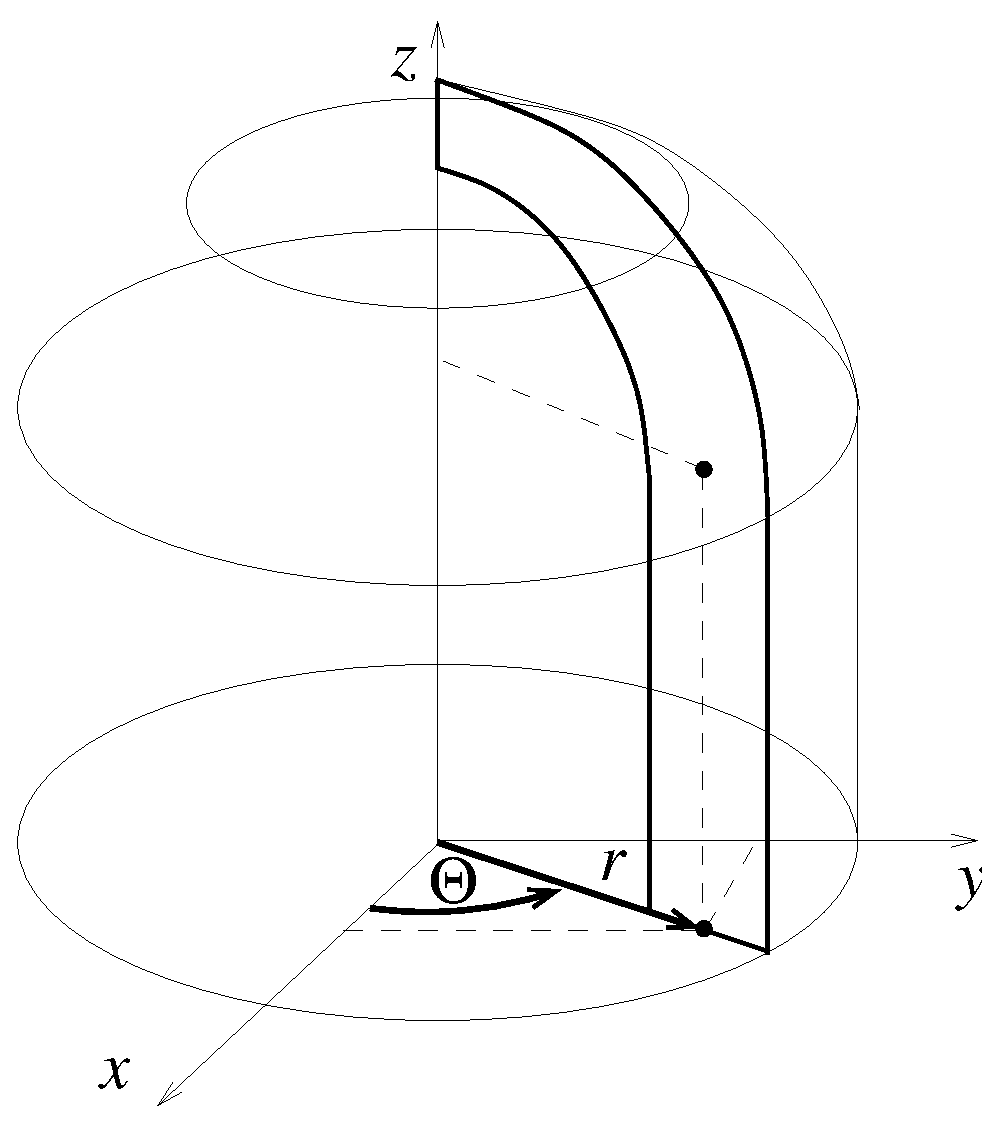
\includegraphics[angle=0, width=6.5cm]{PS/note_axisym.eps}
\caption{Notation for axisymmetric domain}
\label{axisym}
\end{center}
\end{figure}

We start by modifying integral \eqref{nkint}, in which partial derivatives of general shape functions 
$\tenss{N}$ expressed in axisymmetric coordinates (Fig. \ref{axisym}) take this form
\begin{eqnarray}\label{der_ax}
\frac{\partial \tenss{N}}{\partial x} &=&  \frac{\partial \tenss{N}}{\partial r} \frac{\partial r}{\partial x} 
+ \frac{\partial \tenss{N}}{\partial \Theta} \frac{\partial \Theta}{\partial x},\nonumber\\
\frac{\partial\tenss{N} }{\partial y} &=&  \frac{\partial\tenss{N} }{\partial r} \frac{\partial r}{\partial y} 
+ \frac{\partial \tenss{N}}{\partial \Theta} \frac{\partial \Theta}{\partial y},\\
\frac{\partial \tenss{N}}{\partial z} &=&  \frac{\partial \tenss{N}}{\partial z}\nonumber,\\
{\rm d} \Omega &=& {\rm d}x \;{\rm d}y \;{\rm d}z = r \;{\rm d}\Theta \;{\rm d}r \;{\rm d}z,\nonumber
\end{eqnarray}
where
\begin{eqnarray}\label{der_gon}
\frac{\partial r}{\partial x} = \cos \Theta,\quad
\frac{\partial r}{\partial y} = \sin \Theta,\quad
\frac{\partial \Theta}{\partial x} = -\frac{\sin \Theta}{r},\quad
\frac{\partial r}{\partial y} = \frac{\cos \Theta}{r}.
\end{eqnarray}
The first two Eqs.~\eqref{der_ax} can be rewritten as:
\begin{eqnarray}\label{der_n}
\frac{\partial \tenss{N}}{\partial x} =  \frac{\partial \tenss{N}}{\partial r} \cos \Theta 
- \frac{\partial \tenss{N}}{\partial \Theta} \frac{\sin \Theta}{r},\nonumber\\
\frac{\partial \tenss{N}}{\partial y} =  \frac{\partial \tenss{N}}{\partial r} \sin \Theta 
+ \frac{\partial \tenss{N}}{\partial \Theta} \frac{\cos \Theta}{r}.
\end{eqnarray}
Application of Eqs.~\eqref{der_ax} and \eqref{der_n} and subsequent mathematical operations,
lead to integrals expressing the conductivity matrix
\begin{eqnarray}\label{n_int}
\tenss{K} &=& \int_{\Omega} \Big(\frac{\partial \tenss{N}^T}{\partial r} k
\frac{\partial \tenss{N}}{\partial r} \cos^2 \Theta
+ \frac{\partial \tenss{N}^T}{\partial r}k\frac{\partial \tenss{N}}{\partial r} \sin^2 \Theta + 
\frac{\partial \tenss{N}^T}{\partial z}k\frac{\partial \tenss{N}}{\partial z}\Big)
r \;{\rm d}\Theta \;{\rm d}r \;{\rm d}z = \nonumber\\
&=&\int_{\Omega} \Big(\frac{\partial \tenss{N}^T}{\partial r}k\frac{\partial \tenss{N}}{\partial r} + 
\frac{\partial \tenss{N}^T}{\partial z}k\frac{\partial \tenss{N}}{\partial z}\Big)
r \;{\rm d}\Theta \;{\rm d}r \;{\rm d}z,
\end{eqnarray}
where $\tenss{N}$ represents the shape functions of variables $u$ and $k$ stands for the 
material variable. 
The resulting integral formula for the conductivity matrix is obtained after integration 
of \eqref{n_int} with respect to $\Theta$ from 0 to 2$\pi$.
\begin{eqnarray}\label{int_k}
\tenss{K} &=& 2\pi \int_{\Omega} \Big(\frac{\partial \tenss{N}^T}{\partial r}k\frac{\partial \tenss{N}}{\partial r} + 
\frac{\partial \tenss{N}^T}{\partial z}k\frac{\partial \tenss{N}}{\partial z}\Big)
r \;{\rm d}r \;{\rm d}z.
\end{eqnarray}
The capacity matrix and vectors of prescribed fluxes can be treated in a similar manner.
\begin{eqnarray}
\tenss{C} = 2\pi \int_{\Omega} \Big( \tenss{N}^T c\ \tenss{N}\Big) r \;{\rm d}r \;{\rm d}z ,
\end{eqnarray}
\begin{eqnarray}
\overline{\tenss{q}} = 2\pi \int_{\Gamma} \Big(\tenss{N}_q^T  \overline{q}\Big) r \;{\rm d}r \;{\rm d}z,
\end{eqnarray}
where $\overline{q}$ corresponds to the prescribed fluxes.

%%%%%%%%%%%%%%%%%%%%%%%%%%%%%%%%%%%%%%%%%%%%%%%%%%%%%%%%
\subsection{Axisymmetric triangular element with linear approximation functions}
\label{trlaxt}

\begin{center}
\begin{tabular}{|l|l|}
\hline
location & /TRFEL/SRC/linbart.cpp\\
         & /TRFEL/SRC/linbart.h
\\ \hline
number of blocks & 2
\\ \hline
block components & $(k), (c)$
\\ \hline
numer. integration & (1 int. point), (3 int. points)
\\ \hline
nodal DOF & number of transported media
\\ \hline
\end{tabular}
\end{center}

Approximation functions
\begin{eqnarray}
N_1^{(1)} &=& L_1,\nonumber\\
N_2^{(1)} &=& L_2,\nonumber\\
N_3^{(1)} &=& 1-L_1-L_2,
\end{eqnarray}

For more details about approximation functions see GEFEL~\ref{}.

%%%%%%%%%%%%%%%%%%%%%%%%%%%%%%%%%%%%%%%%%%%%%%%%%%%%%%%%
\subsection{Axisymmetric quadrilateral element with bi-linear approximation functions}
\label{qualaxt}


\begin{center}
\begin{tabular}{|l|l|}
\hline
location & /TRFEL/SRC/linbart.cpp\\
         & /TRFEL/SRC/linbart.h
\\ \hline
number of blocks & 2
\\ \hline
block components & $(k), (c)$
\\ \hline
numer. integration & ($2 \times 2$ points), ($2 \times 2$ points)
\\ \hline
nodal DOF & number of transported media
\\ \hline
\end{tabular}
\end{center}

Approximation functions

\begin{eqnarray}
N_1^{(1)} &=& \del{1}{4} (1 + \xi) (1 + \eta),\nonumber\\
N_2^{(1)} &=& \del{1}{4} (1 - \xi) (1 + \eta),\nonumber\\
N_3^{(1)} &=& \del{1}{4} (1 - \xi) (1 - \eta),\nonumber\\
N_4^{(1)} &=& \del{1}{4} (1 + \xi) (1 - \eta),\\
\ppd{N_1^{(1)}}{\xi} &=& \del{1}{4} (1 + \eta),\nonumber\\
\ppd{N_2^{(1)}}{\xi} &=& - \del{1}{4} (1 + \eta),\nonumber\\
\ppd{N_3^{(1)}}{\xi} &=& - \del{1}{4} (1 - \eta),\nonumber\\
\ppd{N_4^{(1)}}{\xi} &=& \del{1}{4} (1 - \eta),\nonumber\\
\ppd{N_1^{(1)}}{\eta} &=& \del{1}{4} (1 + \xi),\nonumber\\
\ppd{N_2^{(1)}}{\eta} &=& \del{1}{4} (1 - \xi),\nonumber\\
\ppd{N_3^{(1)}}{\eta} &=& - \del{1}{4} (1 - \xi),\nonumber\\
\ppd{N_4^{(1)}}{\eta} &=& - \del{1}{4} (1 + \xi).\nonumber
\end{eqnarray}

\chapter{Material models}
\label{matmodels}

%%%%%%%%%%%%%%%%%%%%%%%%%%%%%%%%%%%%%%%%%%%%%%%%%%%%%%%%
%%%%%%%%%%%%%%%%%%%%%%%%%%%%%%%%%%%%%%%%%%%%%%%%%%%%%%%%
\section{General strategy}

Transport processes are based on gradients of suitable variables and on fluxes of mentioned variables.
Connection between gradients and fluxes guarantees constitutive laws. Consider transport of one medium,
e.g. heat. Basic variable is temperature. Gradient of temperature is denoted
\begin{equation}
\mbf{g} = {\rm grad}\ T = \left(\ppd{T}{x},\ \ppd{T}{y},\ \ppd{T}{z}\right)^T\ , \ \ \ \ \
g_i = \ppd{T}{x_i}\ .
\end{equation}
Flux of heat is defined by Fourier's law
\begin{equation}
\mbf{q} = \mbf{D} \mbf{g}\ ,\ \ \ \ \ \
q_i = D_{ij} g_j\ ,
\end{equation}
where $\mbf{D}$ denotes matrix of material coefficients. The simplest Fourier's law uses diagonal matrix $\mbf{D}$
where conduction coefficients are located on the diagonal.
Flux of any quantity is used in conservation law which has form
\begin{equation}
{\rm div} \mbf{q} = 0\ ,\ \ \ \ \ \
\ppd{q_i}{x_i} = 0\ .
\end{equation}

Previously described strategy is valid when one medium is transported. In case of several, say $n$, transported media,
the situation is more complicated. Each of $n$ media has its own macroscopic quantity which defines state of the medium
and is denoted as $f_i$. Gradient of each quantity can be computed and is denoted as
\begin{equation}
\mbf{g}^i = {\rm grad}\ f_i\ ,\ \ \ \ \ \
g_j^i = \ppd{f_i}{x_j}\ .
\end{equation}
Superscript denotes the quantity and subscript denotes the component.
Fluxes of particular quantities are linear combinations of gradients multiplied by material coefficients.
They can be expressed as
\begin{equation}
\mbf{q}^i = \sum_{j=1}^n \mbf{D}_j^i \mbf{g}^j\ ,\ \ \ \ \
q_j^i = D_{jk}^m g_k^m\ .
\end{equation}
The constitutive matrix $\mbf{D}_j^i$ defines interaction between the $i$-th flux and the $j$-th gradient.


%%%%%%%%%%%%%%%%%%%%%%%%%%%%%%%%%%%%%%%%%%%%%%%%%%%%%%%%
%%%%%%%%%%%%%%%%%%%%%%%%%%%%%%%%%%%%%%%%%%%%%%%%%%%%%%%%
\section{Media transfer}
%%%%%%%%%%%%%%%%%%%%%%%%%%%%%%%%%%%%%%%%%%%%%%%%%%%%%%%%

\subsection{One medium transfer}
\label{onemedtrans}
{\bf System of equations:}

\begin{eqnarray}\label{onemed}
\tenss{K}_{11}\tenss{r}_1 + \tenss{C}_{11}\dot{\tenss{r}}_1 = {\tenss{q}}_1
\end{eqnarray}

%%%%%%%%%%%%%%%%%%%%%%%%%%%%%%%%%%%%%%%%%%%%%%%%%%%%%%%%
\subsection{Two media transfer}

{\bf System of equations:}

\begin{eqnarray}
\left[ \begin{array}{cc}
\tenss{K}_{11} & \tenss{K}_{12} \\
\tenss{K}_{21} & \tenss{K}_{22}
\end{array} \right]
\left\{ \begin{array}{c}
\tenss{r}_1 \\
\tenss{r}_{2}
\end{array} \right\} + 
\left[ \begin{array}{cc}
\tenss{C}_{11} & \tenss{C}_{12} \\
\tenss{C}_{21} & \tenss{C}_{22}
\end{array} \right]
\left\{ \begin{array}{c}
\dot{\tenss{r}}_1 \\
\dot{\tenss{r}}_{1}
\end{array} \right\} = 
\left\{ \begin{array}{c}
\tenss{q}_{1} \\
\tenss{q}_{2}
\end{array} \right\}.
\end{eqnarray}

%%%%%%%%%%%%%%%%%%%%%%%%%%%%%%%%%%%%%%%%%%%%%%%%%%%%%%%%
\subsection{Three media transfer}

{\bf System of equations:}

\begin{eqnarray}
\left[ \begin{array}{ccc}
\tenss{K}_{11} & \tenss{K}_{12} & \tenss{K}_{13} \\
\tenss{K}_{21} & \tenss{K}_{22} & \tenss{K}_{23} \\
\tenss{K}_{31} & \tenss{K}_{32} & \tenss{K}_{33}
\end{array} \right]
\left\{ \begin{array}{c}
\tenss{r}_1 \\
\tenss{r}_2 \\
\tenss{r}_3
\end{array} \right\} + 
\left[ \begin{array}{ccc}
\tenss{C}_{11} & \tenss{C}_{12} & \tenss{C}_{13} \\
\tenss{C}_{21} & \tenss{C}_{22} & \tenss{C}_{23} \\
\tenss{C}_{31} & \tenss{C}_{32} & \tenss{C}_{33}
\end{array} \right]
\left\{ \begin{array}{c}
\dot{\tenss{r}}_1 \\
\dot{\tenss{r}}_2 \\
\dot{\tenss{r}}_3
\end{array} \right\} = 
\left\{ \begin{array}{c}
\tenss{q}_1 \\
\tenss{q}_2 \\
\tenss{q}_3
\end{array} \right\}.
\end{eqnarray}



%%%%%%%%%%%%%%%%%%%%%%%%%%%%%%%%%%%%%%%%%%%%%%%%%%%%%%%%
%%%%%%%%%%%%%%%%%%%%%%%%%%%%%%%%%%%%%%%%%%%%%%%%%%%%%%%%
\section{List of material models}
{\bf List of implemented models for heat and moisture transfer}

\begin{itemize}
\item{\bf isotransmat}\\ 
- calculates properties of general isotropic material for linear one medium heat or moisture transfer 
(constant conductivity/permeability and capacity)

\begin{center}
\begin{tabular}{|l|l|}
\hline
location & /TRFEL/SRC/isotrmat.cpp\\
         & /TRFEL/SRC/isotrmat.h
\\ \hline
related files &
\\ \hline
notes & 
\\ \hline
\end{tabular}
\end{center}

\item{\bf cernyconcrete}\\ 
- computes conductivity and capacity coefficients for fiber concrete for one medium heat transfer (one medium, $t$ ... temperature [$^\circ$C])\\
- data measured in the laboratory of the Department of Physics of the Faculty of Civil Engineering CTU Prague

\begin{center}
\begin{tabular}{|l|l|}
\hline
location & /TRFEL/SRC/cerny\_concrete.cpp\\
         & /TRFEL/SRC/cerny\_concrete.h
\\ \hline
related files &
\\ \hline
notes & 
\\ \hline
\end{tabular}
\end{center}

\item{\bf bazantpedersen}\\ 
- computes conductivity and capacity matrices general material for two media coupled heat and moisture transfer (two media - $w$ ... water content [kg/kg], $t$ ... temperature [K])\\
- the theory is based on Lewis' and Schrefler's theory - theory of multi-phase porous medium\\
- water vapor permeability is from Bazant and Najjar (1972)~\cite{bazant_n}\\
- sorption isotherm and hydraulic conductivity is from Pedersen (1990)~\cite{pedersen}

\begin{center}
\begin{tabular}{|l|l|}
\hline
location & /TRFEL/SRC/bazped.cpp\\
         & /TRFEL/SRC/bazped.h
\\ \hline
related files &
\\ \hline
notes & 
\\ \hline
\end{tabular}
\end{center}

\item{\bf pedersen}\\ 
- computes conductivity and capacity matrices general material for two media coupled heat and moisture transfer (two media - $w$ ... water content [kg/kg], $t$ ... temperature [K])\\
- the theory is based on Lewis' and Schrefler's approach - theory of multi-phase porous medium\\
- water vapor permeability is from Pedersen (1990)~\cite{pedersen}\\
- sorption isotherm and hydraulic conductivity is from Pedersen (1990)~\cite{pedersen}

\begin{center}
\begin{tabular}{|l|l|}
\hline
location & /TRFEL/SRC/pedersen.cpp\\
         & /TRFEL/SRC/pedersen.h
\\ \hline
related files &
\\ \hline
notes & 
\\ \hline
\end{tabular}
\end{center}

\item{\bf kunzel}\\ 
- computes conductivity and capacity matrices general material for two media coupled heat and moisture transfer (two media - $h$ ... relative humidity [-], $t$ ... temperature [K])\\
- the theory is based on K${\rm\ddot{u}}$nzel and Kiessl approach~\cite{kunzel}\\
- water vapor permeability is from\\
- sorption isotherm and hydraulic conductivity is from

\begin{center}
\begin{tabular}{|l|l|}
\hline
location & /TRFEL/SRC/kunzel.cpp\\
         & /TRFEL/SRC/kunzel.h
\\ \hline
related files &
\\ \hline
notes & 
\\ \hline
\end{tabular}
\end{center}

\item{\bf models for concrete}\\ 
- computes conductivity and capacity matrices for three media fully coupled heat and moisture transfer in concrete 
(three media - $pc$ ... capillary pressure [Pa], $pg$ capillary gas pressure ... [Pa], $t$ ... temperature [K])\\
- the theory is based on Lewis' and Schrefler's approach - theory of multi-phase porous medium\\
- all of listed models are from Department of Constructions and Transportation Engineering, University of Padua~\cite{pesavento}

\begin{center}
\begin{tabular}{|l|l|}
\hline
location & /TRFEL/SRC/baroghelB.cpp\\
         & /TRFEL/SRC/baroghelB.h\\
         & /TRFEL/SRC/C30baroghel.cpp\\
         & /TRFEL/SRC/C30baroghel.h\\
         & /TRFEL/SRC/C60baroghel.cpp\\
         & /TRFEL/SRC/C60baroghel.h\\
         & /TRFEL/SRC/C60bazant.cpp\\
         & /TRFEL/SRC/C60bazant.h\\
         & /TRFEL/SRC/concreteB.cpp\\
         & /TRFEL/SRC/concreteB.h\\
         & /TRFEL/SRC/o30bazant.cpp\\
         & /TRFEL/SRC/o30bazant.h
\\ \hline
related files & /TRFEL/SRC/constrel.cpp\\
              & /TRFEL/SRC/constrel.h\\
              & /TRFEL/SRC/multiphase.cpp\\
              & /TRFEL/SRC/multiphase.h
\\ \hline
notes & not working at high temperatures (still tested) 
\\ \hline
\end{tabular}
\end{center}

\item{\bf glasgow}\\ 
- computes conductivity and capacity matrices for three media fully coupled heat and moisture transfer in concrete 
(three media - $\widetilde{\rho}_V$ ... concentration of water vapor [kg/m$^3$], $pg$ capillary gas pressure ... [Pa], $t$ ... temperature [K])\\
- the theory is based on Tenchev approach~\cite{tenchev} and \cite{glas}(\textsf {http://cml.fsv.cvut.cz/\~{}sifel}).

\begin{center}
\begin{tabular}{|l|l|}
\hline
location & /TRFEL/SRC/glasgowmat.cpp\\
         & /TRFEL/SRC/glasgowmat.h
\\ \hline
related files &
\\ \hline
notes &  not working at high temperatures (still tested) 
\\ \hline
\end{tabular}
\end{center}

\end{itemize}

%%%%%%%%%%%%%%%%%%%%%%%%%%%%%%%%%%%%%%%%%%%%%%%%%%%%%%%%
%%%%%%%%%%%%%%%%%%%%%%%%%%%%%%%%%%%%%%%%%%%%%%%%%%%%%%%%
\section{Models for heat transfer}
\subsection{Models for effective heat conductivity and capacity}
\subsubsection{Cerny model}

\begin{center}
\begin{tabular}{|l|l|}
\hline
location & /TRFEL/SRC/cerny\_concrete.cpp\\
         & /TRFEL/SRC/cerny\_concrete.h
\\ \hline
related files &
\\ \hline
notes & 
\\ \hline
\end{tabular}
\end{center}


Thermo-physical parameters of given concrete were measured in the laboratory 
of the Department of Physics of the Faculty of Civil Engineering CTU in Prague~\cite{cerny}:
\begin{eqnarray}
\chi_{\rm eff} &=& (2.3670 - 0.0028 T) \quad {\rm W/(m K)}, \qquad T \in \langle 20^{\circ}{\rm C}, 
90^{\circ}{\rm C}\rangle, \\
C_{\rm eff} &=& (850 + 0.25 T) \quad {\rm J/(kg K)}, \qquad \qquad \;\; T\in \langle 20^{\circ}{\rm C}, 
90^{\circ}{\rm C}\rangle, \\
\rho &=& 2280 \quad {\rm kg/m}^3.\nonumber
\end{eqnarray}


%%%%%%%%%%%%%%%%%%%%%%%%%%%%%%%%%%%%%%%%%%%%%%%%%%%%%%%%

%%%%%%%%%%%%%%%%%%%%%%%%%%%%%%%%%%%%%%%%%%%%%%%%%%%%%%%%
%%%%%%%%%%%%%%%%%%%%%%%%%%%%%%%%%%%%%%%%%%%%%%%%%%%%%%%%
\section{Models for moisture transfer}

%%%%%%%%%%%%%%%%%%%%%%%%%%%%%%%%%%%%%%%%%%%%%%%%%%%%%%%%
\subsection{Models for moisture storage function}
Porous materials have the capability of absorbing moisture from an environment of air due to adsorption forces, 
attracting molecules of vapor to the solid parts of the porous system, and due to the depression of water pressure 
because of the tension over the concave menisci of the water filled capillaries. Moisture in materials can be therefore 
present as moist air, water and ice or in some intermediate state 
as adsorbed phase on the pore walls, respectively. Since it is in general not possible to distinguish the different 
aggregate states, the water content is defined as the ratio of the total moisture weight to the dry weight 
of the material \cite{ctu}. Equilibrium of the water content with its local environment is represented by a retention curve 
of the material, relating the moisture and the relative humidity $h$ of the surrounding air. 

The {\it moisture retention curve} is composed of three parts Fig.~(\ref{reten}): 
the {\it sorption isotherm} up to about 95 \% 
- 98 \% relative humidity $RH$ (region I), the capillary moisture (region II), and the over-saturated region III, where 
the water retention function is a vertical line at 100 \% $RH$. As is demonstrated in Fig.~\ref{reten}, a higher 
temperature level results in lower moisture content for the same relative humidity. In the region II it is difficult 
to determine $w$ unambiguously by sorption tests. However, there still exists equilibrium between two porous materials 
up to the capillary saturation with a suction stress close to zero (a material is in contact with liquid water). 
In order to fill all pores, a high pressure or vacuum has to be applied in the region III. In this region, 
no well-defined function exists between the water content and the relative humidity or the suction stress, respectively, 
and therefore, no well-defined moisture equilibrium between two porous material samples might be expected.
\begin{figure}[h!]
\begin{center}
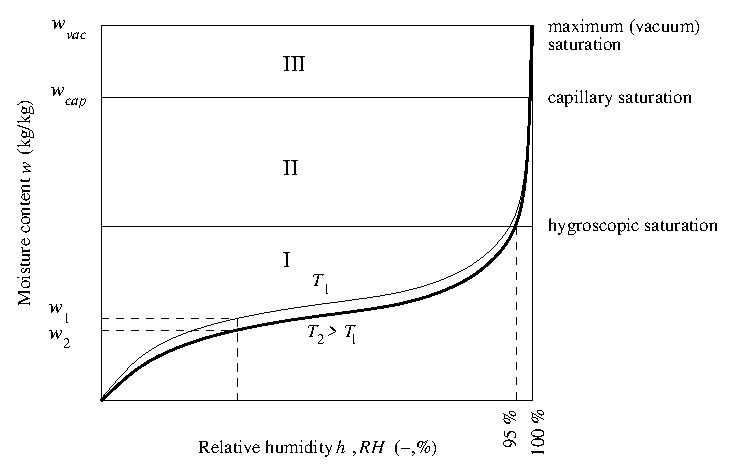
\includegraphics[angle=0, width=10cm]{PS/reten.eps}
\caption{Sorption isotherms}
\label{reten}
\end{center}
\end{figure}

In the transient region II, there is a relationship between the relative humidity, the water content (saturation) 
and the capillary pressure in the pores \cite{lewis}
\begin{eqnarray}\label{cap_press}
p^c = p^g - p^w,
\end{eqnarray}
where $p^w > 0$ is the pressure of the liquid phase (water). 

\subsubsection{Pedersen model}

\begin{center}
\begin{tabular}{|l|l|}
\hline
location & /TRFEL/SRC/bazped.cpp\\
         & /TRFEL/SRC/bazped.h\\
         & /TRFEL/SRC/pedersen.cpp\\
         & /TRFEL/SRC/pedersen.h
\\ \hline
related files &
\\ \hline
notes & 
\\ \hline
\end{tabular}
\end{center}

The sorption isotherm is approximated by this simple formula \cite{pedersen}
\begin{eqnarray}\label{sorption_isotherm}
w = w_h \Big(1 - \frac{\ln h}{A}\Big)^{-\frac{1}{n}},
\end{eqnarray}
where $h$ is relative humidity and $w_h$, $A$, $n$ are material parameters.

An analytical expression is proposed for the saturation vapor pressure as a function of temperature $T[{\rm K}]$ 
\begin{eqnarray}\label{saturation_pressure}
p^{gws}(T) = \exp \Big(23,5771 - \frac{4042,9}{T-37,58}\Big) \quad ({\rm Pa}).
\end{eqnarray}

\subsubsection{JM model}
\begin{center}
\begin{tabular}{|l|l|}
\hline
location & /TRFEL/SRC/kunzel.cpp\\
         & /TRFEL/SRC/kunzel.h
\\ \hline
related files &
\\ \hline
notes & 
\\ \hline
\end{tabular}
\end{center}


%%%%%%%%%%%%%%%%%%%%%%%%%%%%%%%%%%%%%%%%%%%%%%%%%%%%%%%%
\subsection{Models for water vapor permeability}
As for the {\it water vapor transport}, studies of experimental data of concrete have indicated that permeability 
varies tremendously with temperature especially at temperature levels close to 100$^\circ$C. 
Introducing water vapor permeabilty as a scalar variable,
\begin{eqnarray}
\delta^{gw} = \frac{k^{rgw}k_{sat}}{\nu^{gw}} \quad ({\rm s}),
\end{eqnarray}
and denoting its maximum as $\delta_{wet}^{gw}$, the two possible diagrams of the water vapor permeability displayed 
in Fig.~\ref{s_shape} as a function of relative humidity  $RH = h$ and moisture content $w$, respectively, 
are plausible approximations of this dependence.
\begin{figure}[h!]
\begin{center}
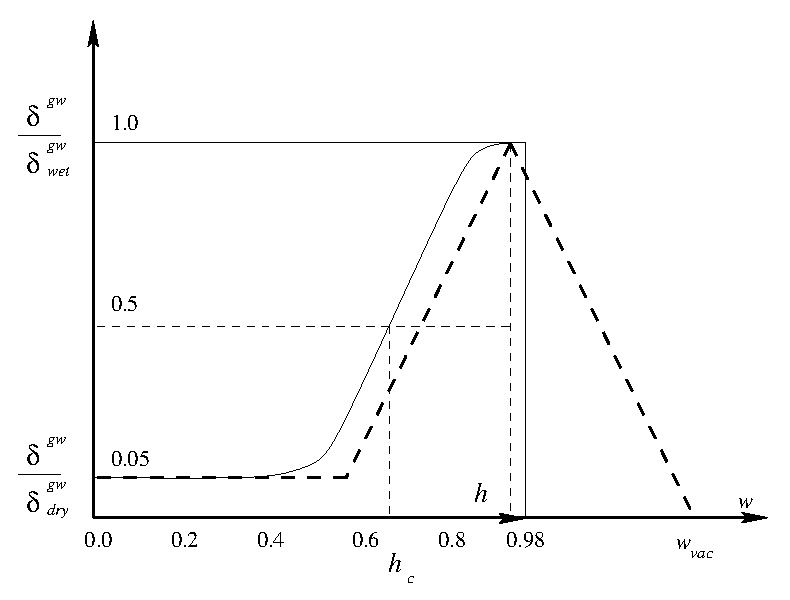
\includegraphics[angle=0, width=10cm]{PS/s_shape.eps}
\caption{Distribution of water vapor permeability as a function of $h$ and $w$}
\label{s_shape}
\end{center}
\end{figure}

\subsubsection{Bazant model}

\begin{center}
\begin{tabular}{|l|l|}
\hline
location & /TRFEL/SRC/bazped.cpp\\
         & /TRFEL/SRC/bazped.h
\\ \hline
related files &
\\ \hline
notes & 
\\ \hline
\end{tabular}
\end{center}

The solid S-shaped curve was proposed by Z. P. Ba\v{z}ant and L. J. Njjar in~\cite{bazant_n} using a function 
with three parameters $a_0$, $h_c$, $n$
\begin{equation}
\frac{\delta^{gw}}{\delta_{\rm wet}^{gw}} = a_0 + \frac{1 -a_0}{1 + \big(\frac{1 - h}{1 - h_c}\big)^n},
\end{equation}
where parameter $h_c$ characterizes the relative humidity at which $\delta^{gw}/\delta_{wet}^{gw}$ drops half-way between 
its maximum and minimum values. The dashed line was considered by \cite{pedersen}.


\subsubsection{Pedersen model}

\begin{center}
\begin{tabular}{|l|l|}
\hline
location & /TRFEL/SRC/pedersen.cpp\\
         & /TRFEL/SRC/pedersen.h
\\ \hline
related files &
\\ \hline
notes & 
\\ \hline
\end{tabular}
\end{center}

The dashed line was considered by \cite{pedersen}:
\begin{equation}
\delta^{gw} = \delta^{gw}_{\rm dry} + \frac{h-0.60}{0.98-h}(\delta^{gw}_{\rm wet} - \delta^{gw}_{\rm dry}),\nonumber
\end{equation}
if $h$ $\leq$ 0.60:
\begin{equation}
\delta^{gw} = \delta^{gw}_{\rm dry},\nonumber
\end{equation}
if $h$ $\geq$ 0.98:
\begin{equation}
\delta^{gw} = \delta^{gw}_{\rm wet}\frac{w_{\rm cap} - w}{w_{\rm vac} - w_{98}},\nonumber
\end{equation}
if $w$ $>$ $w_{\rm vac}$:
\begin{equation}
\delta^{gw} = 0.\nonumber
\end{equation}

%%%%%%%%%%%%%%%%%%%%%%%%%%%%%%%%%%%%%%%%%%%%%%%%%%%%%%%%
\subsection{Models for hydraulic conductivity}
\subsubsection{Pedersen model}

\begin{center}
\begin{tabular}{|l|l|}
\hline
location & /TRFEL/SRC/bazped.cpp\\
         & /TRFEL/SRC/bazped.h\\
         & /TRFEL/SRC/pedersen.cpp\\
         & /TRFEL/SRC/pedersen.h
\\ \hline
related files &
\\ \hline
notes & 
\\ \hline
\end{tabular}
\end{center}

For the {\it liquid transport} the following expressions are proposed in \cite{pedersen} to describe, 
in case of uniaxial flow, the dependence of the so called hydraulic conductivity, $K^w/g$ (s), 
on the moisture content $w$:
\begin{equation}\label{20}
\begin{array}{rl} 
w < w_{cr}, & K^w/g \doteq 0,\\
w_{cr} \leq w \leq w_{cap}, & K^w/g = A_k {\rm exp} \big(B_kw \big),\\
w_{cap} < w, & K^w/g = A_k {\rm exp} \big(B_kw_{cap} \big),
\end{array}
\end{equation}
where $A_k,B_k$ are coefficients yet to be determined from experiments.


%%%%%%%%%%%%%%%%%%%%%%%%%%%%%%%%%%%%%%%%%%%%%%%%%%%%%%%%
%%%%%%%%%%%%%%%%%%%%%%%%%%%%%%%%%%%%%%%%%%%%%%%%%%%%%%%%
\section{Models for coupled heat and moisture transfer}
\subsection{Mass and heat transfer in deforming porous media \\- a review of Lewis' and Schrefler's theory}
\label{keynote}
{\bf Constitutive relations}

Moisture in materials can be present as moist air, water and ice or in some intermediate state as adsorbed phase 
on the pore walls, respectively. Since it is in general not possible to distinguish the different aggregate states, 
the water content $w$ is defined as the ratio of the total moisture weight (kg/kg) to the dry weight of the material. 
\begin{eqnarray}\label{w_S}
(1-n) \rho^sw = nS_w\rho^w + nS_g\rho^g, \qquad S_w + S_g = 1,
\end{eqnarray}
The degree of saturation $S_w$ is a function of capillary pressure $p^c$ and temperature $T$, 
which is determined experimentally
\begin{equation}\label{Sw}
S_w = S_w(p^c,T).
\end{equation}
The capillary pressure $p^c$ id defined as
\begin{equation}\label{pc}
p^c = p^g - p^w,
\end{equation}
where $p^w > 0$ is the pressure of the liquid phase (water). 

The pressure of the moist air, $p^g > 0$, in the pore system is usually considered as the pressure in a perfect 
mixture of two ideal gases - dry air, $p^{ga}$, and water vapor, $p^{gw}$, i.e.,
\begin{equation}\label{ungas}
p^g = p^{ga} + p^{gw}=\Big( \frac{\rho^{ga}}{M_a} + \frac{\rho^{gw}}{M_w} \Big)T 
R = \frac{\rho^{g}}{M_g}T R.
\end{equation}
In this relation $\rho^{ga}, \rho^{gw}$ and $\rho^{g}$ stand for the respective intrinsic phase densities, $T$ 
is the absolute temperature, and $R$ is the universal gas constant.
 
Identity \eqref{ungas} defining the molar mass of the moist air, $M_g$, in terms of the molar masses of individual 
constituents is known as Dalton's law. The capillary pressure is larger the smaller the capillary radius is. It is shown 
thermodynamically that the capillary pressure can be expressed unambiguously by the relative humidity $RH$ using 
the Kelvin-Laplace law
\begin{equation}\label{kelvinlapl}
RH = \frac{p^{gw}}{p^{gws}} = {\rm exp} \Big( - \frac{p^c M_w}{\rho^w R T} \Big).
\end{equation}
The water vapor saturation pressure, $p^{gws}$, is a function of the temperature only and can be expressed by the 
Clausius-Clapeyron equation
\begin{equation}\label{clausius}
p^{gws}(T) = p^{gws}(T_0) {\rm exp} \Big[ - \frac{M_w \Delta h_{\rm vap}}{R} \Big(\frac{1}{T} - 
\frac{1}{T_0} \Big) \Big],
\end{equation}
where $T_0$ is a reference temperature and $\Delta h_{\rm vap}$ is the specific enthalpy of saturation.

Materials having heat capacities is the term deliberately used 
to emphasize the similarity to the description of the moisture retention. It is simply expressed as
\begin{equation}
H =H(T),
\end{equation}
where $H$ is the mass specific enthalpy (J.kg$^{-1}$), $T$ - temperature (K).

It is not common to write the enthalpy in an absolute way as here. Instead, changes of enthalpy are 
described in a differential way, which leads to the definition of the specific heat capacity as the slope 
of the $H - T$ curve, i.e.
\begin{equation}\label{cap}
C_p = \Big( \frac{\partial H}{\partial T}\Big)_{p={\rm const.}}.
\end{equation}
The heat capacity varies insignificantly with temperature. It is customary, however, to correct this term 
for the presence of the fluid phases and to introduce the effective heat capacity as
\begin{equation}
\big( \rho C_p \big)_{\rm eff} = \rho_s C_{ps} + \rho_w C_{pw} + \rho_g C_{pg}.
\end{equation}

{\bf Transfer equations}

The mass averaged relative velocities, $\tenss{v} ^{\alpha} - \tenss{v} ^s$, are expressed 
by the generalized form of {\bs {Darcy's law}} \cite{lewis}
\begin{equation}\label{darcy}
n S_{\alpha} \big( \tenss{v} ^{\alpha} - \tenss{v} ^s \big) = \frac{k^{r\alpha} \tenss{k}_{sat}}
{\mu^{\alpha}} \big( - {\rm grad} p^{\alpha} + \rho^{\alpha} \tenss{g} \big),
\end{equation}
where $\alpha = w$ for the liquid phase and $\alpha = g$ for the gaseous phase.

Dimensionless relative permeabilities $k^{r\alpha} \in \langle 0,1 \rangle$ are functions of degree of~
saturation
\begin{equation}
k^{r\alpha} = k^{r\alpha} (S_w)\qquad ({\rm m \cdot s}^{-1}).
\end{equation}

In Equation (\ref{darcy}), $\tenss{k}_{sat}$ (m$^2$) is the square (3x3) intrinsic permeability matrix 
 and $\mu^{\alpha}$ is the dynamic viscosity (kg.m$^{-1}$.s$^{-1}$). The intrinsic mass densities $\rho^{\alpha}$ 
are related to the volume averaged mass densities $\rho_{\alpha}$ through the relation
\begin{equation}\label{av_dens}
\rho_{\alpha} = n S_{\alpha} \rho^{\alpha}.
\end{equation}
The relative permeability $k^{rw}$ goes to zero, when water saturation $S_w$ approaches $S_{irr}$, 
which is the limiting value of $S_w$ as the suction stress approaches infinity (\cite{fatt}).

Diffusive-dispersive mass flux (kg.m$^{-2}$.s$^{-1}$) of the water vapor ($gw$) in the gas
 ($g$) is the second driving mechanism. It is governed by {\bs {Fick's law}}
\begin{equation}\label{fick}
\tenss{J}^{gw}_g = n S_g \rho^{gw} \big( \tenss{v} ^{gw} - \tenss{v} ^g \big) = - \rho^g \tenss{D}^{gw}_g 
{\rm grad} \Big( \frac{\rho^{gw}}{\rho^g} \Big),
\end{equation}
where $\tenss{D}^{gw}_g$ (m$^2$.s$^{-1}$) is the effective dispersion tensor. It can be shown \\ \cite{lewis} that
\begin{equation}
\tenss{J}^{gw}_g = - \rho^g \frac{M_a M_w}{M^2_g} \tenss{D}^{gw}_g {\rm grad} \Big( \frac{\rho^{gw}}{\rho^g} \Big)
= \rho^g \frac{M_a M_w}{M^2_g} \tenss{D}^{ga}_g {\rm grad} \Big( \frac{\rho^{ga}}{\rho^g} \Big) = - \tenss{J}^{ga}_g.
\end{equation}
Recall that $\tenss{D}^{gw}_g = \tenss{D}^{ga}_g = \tenss{D}_g$.
Here, $\tenss{J}_g^{ga}$ is the diffusive-dispersive mass flux of the dry air in the gas.

Conduction of heat in normal sense comprises radiation as well as convective heat transfer on a 
microscopic level. The generalized version of {\bs {Fourier's law}} is used to describe the conduction
 heat transfer
\begin{equation}\label{fourier}
\tenss{q} = - \tenss{\chi}_{\rm eff} {\rm grad} T,
\end{equation}
where $\tenss{q}$ is the heat flux (W.m$^{-2}$), $\tenss{\chi}_{\rm eff}$ is the effective thermal conductivity matrix 
(W.m$^{-1}$.K$^{-1}$).

The thermal conductivity increases with increasing temperature due to the non-linear 
behavior of the microscopic radiation, which depends on difference of temperatures raised to the 
$4^{\rm{th}}$ power. Presence of water also increases the thermal conductivity. A suitable formula
reflecting this effect can be found in \cite{lewis}.

{\bf Deformation of solid skeleton. Concept of effective stress}

The stresses in the grains, $\tenss{\sigma}^s$, can be expressed using a standard averaging technique 
in terms of the stresses in the liquid phase, $\tenss{\sigma}^w$, the stresses in the gas, $\tenss{\sigma}^g$, 
and the effective stresses between the grains, $\tenss{\sigma}^{ef}$. The equivalence conditions for the internal 
stresses and for the total stress $\tenss{\sigma}$ lead to the expression~\cite{bitt}.
\begin{equation}\label{d3}
\tenss{\sigma} = \tenss{\sigma}^{ef} + S_w \tenss{\sigma}^w + S_g \tenss{\sigma}^g + \Delta \tenss{\tau}.
\end{equation}
Assuming that the shear stress $\tenss{\tau}$ in fluids is negligible converts the latter equation into the form
\begin{equation}\label{d4}
\tenss{\sigma} = \tenss{\sigma}^{ef} - p^s \tenss{m},
\end{equation}
where
\begin{equation}\label{d5}
\tenss{\sigma} = \big\{ \sigma_x,\sigma_y,\sigma_z,\tau_{yz},\tau_{zx},\tau_{xy}\big\}^{\rm T}, \quad
\tenss{m} = \big\{ 1,1,1,0,0,0 \big\}^{\rm T},
\end{equation}
and
\begin{equation}\label{d6}
p^s = S_w p^w + S_g p^g.
\end{equation}

Deformation of a porous skeleton associated with the grain rearrangement can be expressed using 
the constitutive equation written in the rate form
\begin{equation}\label{d7}
\dot{\tenss{\sigma}}^{ef} = \tenss{D}_{sk} \big(\dot{\tenss{\varepsilon}} - \dot{\tenss{\varepsilon}}_0 \big).
\end{equation}
The dots denote differentiation with respect to time, $\tenss{D}_{sk} = \tenss{D}_{sk}(\dot{\tenss{\varepsilon}}, 
{\tenss{\sigma}}^{ef}, T) $ is the tangential matrix of the porous skeleton and $\dot{\tenss{\varepsilon}}_0$ 
represents the strains that are not directly associated with stress changes (e.g., temperature effects, shrinkage, 
swelling, creep). It also comprises the strains of the bulk material due to changes of the pore pressure
\begin{equation}\label{d8}
\dot{\tenss{\varepsilon}} =  -\tenss{m} \Big( \frac{\dot{p}^s}{3K_s} \Big),
\end{equation}
where $K_s$ is the bulk modulus of the solid material (matrix).

When admitting only this effect and combining Equations (\ref{d4}), (\ref{d7}) and (\ref{d8}), we get
\begin{equation}\label{d9}
\dot{\tenss{\sigma}} = \dot{\tenss{\sigma}}^{ef} - \dot{p}^s \tenss{m} = \tenss{D}_{sk} \dot{\tenss{\varepsilon}}
- \alpha \tenss{m} \dot{p}^s = \dot{\tenss{\sigma}}'' - \alpha \tenss{m} \dot{p}^s,
\end{equation}
where
\begin{equation}\label{d10}
\alpha = \frac{1}{3} \tenss{m}^{\rm T} \Big( \tenss{I} - \frac{\tenss{D}_{sk}}{3K_m} \Big) \tenss{m} = 1 - 
\frac{K_{sk}}{K_s} < 1,
\end{equation}
and $K_{sk} = \tenss{m}^{\rm T} \tenss{D}_{sk} \tenss{m}/9$ is the bulk modulus of the porous skeleton. 
For a material without any pores, $K_{sk} = K_s$. For cohesive soils, $K_{sk} << K_s$ and $\alpha = 1$. 
The above formulas are also applicable to long-term deformation of rocks, for which  $\alpha \leq 0.5$, 
and this fact strongly affects Equation (\ref{d9}) \cite{zienkiewicz83}.

Changes of the effective stress along with temperature and pore pressure changes produce change of the solid density 
$\dot{\rho}^s$. To derive the respective material relation for this quantity, we start from the mass conservation equation 
for the solid phase. In the second step we introduce the constitutive relationship for the mean effective stress expressed 
in terms of quantities describing the deformation of the porous skeleton. After some manipulations we arrive at the 
searched formula
\begin{equation}\label{d15}
(1 - n)\frac {\dot{\rho}^s}{\rho^s} = (\alpha - n)\Big(\frac {\dot{p}^s}{K_s} - \beta_s \dot{T}\Big) + 
(\alpha - 1){\rm div} \tenss{v}^s,
\end{equation}
where $\beta_s$ is the thermal expansion coefficient of the solid phase.

Similar approach applied to the mass conservation equation of the liquid phase leads to the following constitutive equation
\begin{equation}\label{d16}
\frac {\dot{\rho}^w}{\rho^w} = \frac {\dot{p}^w}{K_w} - \beta_s \dot{T},
\end{equation}
where $K_w$ is the bulk modulus of water and $\beta_w$ is the thermal expansion coefficient of this phase.

{\bf Set of governing equations}

The complete set of equations describing the coupled moisture and heat transport in deforming porous media comprises 
the linear balance (equilibrium) equation formulated for a multi-phase body, the energy balance equation and 
the continuity equations for the liquid water and gas.

{\it Continuity equation for the dry air}
\begin{eqnarray}\label{air}
\frac{\partial}{\partial t}\Big(\varphi(1-S_w)\rho^{ga}\Big) + \alpha(1-S_w)\rho^{ga} {\rm div} \tenss{\dot{u}} - 
{\rm div} \Big( \rho^{ga}\frac{k^{rg}\tenss{k}_{sat}}{{\mu}^{g}} {\rm grad}p^g\Big) + \nonumber\\
+{\rm div} \Big( \rho^g \frac{M_a M_w}{M^2_g} \tenss{D}_{\rm eff} {\rm grad} \Big( \frac{p^{gw}}{p^g} \Big) \Big) = 0,
\end{eqnarray}
where $\tenss{\dot{u}}$ ($\tenss{\dot{u}} = \tenss{v}^s$) is the velocity of solid.

{ \it Continuity equation for the water species}
\begin{eqnarray}\label{water}
\frac{\partial}{\partial t}\Big(\varphi(1-S_w)\rho^{gw}\Big) + \alpha(1-S_w)\rho^{gw} {\rm div} \tenss{\dot{u}} - 
{\rm div} \Big( \rho^{gw}\frac{k^{rg}\tenss{k}_{sat}}{{\mu}^{g}} {\rm grad}p^g\Big) + \nonumber\\
-{\rm div} \Big( \rho^g \frac{M_a M_w}{M^2_g} \tenss{D}_{\rm eff} {\rm grad} \Big( \frac{p^{gw}}{p^g} \Big) \Big) = \nonumber\\
=-\frac{\partial}{\partial t}\Big(\varphi S_w\rho^{w}\Big) - \alpha S_w \rho^{w} {\rm div} \tenss{\dot{u}} + 
{\rm div} \Big( \rho^{w}\frac{k^{rw}\tenss{k}_{sat}}{{\mu}^{w}} ({\rm grad}p^g - {\rm grad}p^c - \rho^w\tenss{g})\Big)
\end{eqnarray}

{ \it Energy balance equation}
 \begin{eqnarray}\label{heat}
\big( \rho C_p \big)_{\rm eff} \frac{\partial T}{\partial t} - {\rm div}\big(\lambda_{\rm eff}{\rm grad}T\big) + \nonumber\\
- \Big(C_{pw} \rho^w \frac{k^{rw}\tenss{k}_{sat}}{{\mu}^{w}} ({\rm grad}p^g - {\rm grad}p^c - \rho^w\tenss{g}) + 
C_{pg} \rho^{gw}  \frac{k^{rg}\tenss{k}_{sat}}{{\mu}^{g}} {\rm grad}p^g\Big) {\rm grad}T = \nonumber\\
=\Delta h_{\rm vap} \Big[\frac{\partial}{\partial t}\Big(\varphi S_w\rho^{w}\Big) + \alpha S_w \rho^{w} {\rm div} \tenss{\dot{u}} -
{\rm div} \Big( \rho^{w}\frac{k^{rw}\tenss{k}_{sat}}{{\mu}^{w}} ({\rm grad}p^g - {\rm grad}p^c - \rho^w\tenss{g})\Big)\Big]
\end{eqnarray}

The { \it equilibrium equation} (the linear balance equation) must yet be introduced to complete a set of governing 
equations
\begin{equation}\label{d19}
{\rm div} \big(\tenss{\sigma} - \tenss{m}(p^g - S_w p^c)\big)+ \rho \tenss{g} = \tenss{\rm 0}
\end{equation}
with density of the multi-phase medium defined as
\begin{equation}\label{d20}
\rho = (1-n)\rho^s + nS_w\rho^w + nS_g\rho^g = \rho_s + \rho_w + \rho_g.
\end{equation}

{ \it Initial and boundary conditions}

The initial conditions specify the full fields of gas pressure, capillary or water pressure, 
temperature and displacement and velocities:
\begin{equation}\label{init}
p^g = p^g_0, \qquad p^c = p^c_0, \qquad T = T_0, \qquad \tenss{u} = \tenss{u}_0, 
\quad {\rm and}  \quad \dot{\tenss{u}} = \dot{\tenss{u}}_0, \quad {\rm at}\quad t = 0. 
\end{equation}
The boundary conditions can be imposed values on $\Gamma^1_{\pi}$ or fluxes on $\Gamma^2_{\pi}$, where the boundary
$\Gamma = \Gamma^1_{\pi} + \Gamma^2_{\pi}$.
\begin{equation}\label{bound1}
p^g = \overline{p}^g \quad {\rm on} \quad \Gamma^1_{g}, \quad p^c = \overline{p}^c \quad {\rm on} \quad \Gamma^1_{c},
\quad T = \overline{T} \quad {\rm on} \quad \Gamma^1_{T}, \quad \tenss{u} = \overline{\tenss{u}}  \quad {\rm on} \quad \Gamma^1_{u}.
\end{equation}
The volume averaged flux boundary conditions for water species and dry air conservation equations 
and energy equation to be imposed at the interface between the porous medium and the surrounding fluid are as follows
\begin{eqnarray}\label{bound2}
\big(\rho^{ga}\tenss{J}^{ga} - \rho^{g}\tenss{J}^{gw}\big)\cdot\tenss{n} &=& q_{ga} \quad {\rm on} \quad \Gamma^2_{g}\nonumber\\
\big(\rho^{gw}\tenss{J}^{ga} + \rho^{w}\tenss{J}^{w} + \rho^{g}\tenss{J}^{gw}\big)\cdot\tenss{n} &=& 
\beta_c(\rho^{gw} -\rho^{gw}_{\infty}) + q_{gw} + q_{w}\quad {\rm on} \quad \Gamma^2_{c}\\
-\big(\rho^{w}\tenss{J}^{w}\Delta h_{\rm vap} - \lambda_{\rm eff}{\rm grad}T)\cdot\tenss{n} &=& 
\alpha_c(T - T_{\infty}) + q_{T}\quad {\rm on} \quad \Gamma^2_{T}\nonumber
\end{eqnarray}
where $\tenss{n}$ is the unit normal vector of the surface of the porous medium, $\rho^{gw}_{\infty}$ and $T_{\infty}$ 
are the mass concentration of water vapor and temperature in the undisturbed gas phase far away from the interface, 
and $q_{ga}$, $q_{gw}$, $q_w$ and $q_T$ are the imposed air flux, the imposed vapor flux, the imposed liquid flux and 
the imposed heat flux, respectively.

The traction boundary conditions for displacement field are:
\begin{equation}\label{bound3}
\sigma\cdot\tenss{n} = \tenss{t} \quad {\rm on} \quad \Gamma^2_{u}
\end{equation}
where $\tenss{t}$ is the imposed traction.

\subsubsection{Discretization of governing equations}

A weak formulation of the governing equations \eqref{air} to \eqref{d19} is obtained by applying Galerkin's method
of weighted residuals. For the numerical solution, the governing equations are discretized in space by means of the 
finite element method, yielding a non-symmetric and non-linear system of partial differential equations:
\begin{eqnarray}\label{final1}
\tenss{K}_{uu}\tenss{u} + \tenss{K}_{ug}\tenss{p}_g + \tenss{K}_{uc}\tenss{p}_c + \tenss{K}_{ut}\tenss{T} &=& \tenss{F}_u,\nonumber\\
\tenss{C}_{gg}\tenss{\dot{p}}_g + \tenss{C}_{gc}\tenss{\dot{p}}_c + \tenss{C}_{gt}\tenss{\dot{T}} +\tenss{C}_{gu}\tenss{\dot{u}} + 
\tenss{K}_{gg}\tenss{p}_g + \tenss{K}_{gc}\tenss{p}_c + \tenss{K}_{gt}\tenss{T} &=& \tenss{F}_g,\nonumber\\
\tenss{C}_{cg}\tenss{\dot{p}}_g + \tenss{C}_{cc}\tenss{\dot{p}}_c + \tenss{C}_{ct}\tenss{\dot{T}} + \tenss{C}_{cu}\tenss{\dot{u}} + 
\tenss{K}_{cg}\tenss{p}_g + \tenss{K}_{cc}\tenss{p}_c + \tenss{K}_{ct}\tenss{T} &=& \tenss{F}_c,\\
\tenss{C}_{tg}\tenss{\dot{p}}_g + \tenss{C}_{tc}\tenss{\dot{p}}_c + \tenss{C}_{tt}\tenss{\dot{T}} + \tenss{C}_{tu}\tenss{\dot{u}} + 
\tenss{K}_{tg}\tenss{p}_g + \tenss{K}_{tc}\tenss{p}_c + \tenss{K}_{tt}\tenss{T} &=& \tenss{F}_t.\nonumber
\end{eqnarray}
The equations \eqref{final1} can be rewritten in concise form as
\begin{equation}\label{final2}
\tenss{K}(\tenss{X})\tenss{X} + \tenss{C}(\tenss{X})\tenss{\dot{X}} = \tenss{F}(\tenss{X}),
\end{equation}
where $\tenss{X}^{\rm T} = \{\tenss{p}^g,\tenss{p}^c,\tenss{T},\tenss{u}\}$, $\tenss{C}(\tenss{X})$ is ``the general capacity matrix'', 
$\tenss{K}(\tenss{X})$ is ``the general conductivity matrix'' and are obtained together with $\tenss{F}(\tenss{X})$ 
by assembling the sub-matrices indicated in equations \eqref{final1}. The dot denotes the time derivative.


The matrices appearing in Equation \eqref{final1} are shown here in detail in~\cite{pesavento}\\
(\textsf {http://cml.fsv.cvut.cz/\~{}sifel}), using the notation of Lewis and Schrefler~\cite{lewis}.
%\begin{eqnarray}
%\tenss{K}_{uu} &=&\\
%\tenss{K}_{ug} &=&\\
%\tenss{K}_{uc} &=&\\
%\tenss{K}_{ut} &=&\\
%\tenss{F}_u &=&\\
%\tenss{C}_{gg} &=&\\
%\tenss{C}_{gc} &=&\\
%\tenss{C}_{gt} &=&\\
%\tenss{C}_{gu} &=&\\ 
%\tenss{K}_{gg} &=&\\
%\tenss{K}_{gc} &=&\\
%\tenss{K}_{gt} &=&\\
%\tenss{F}_g &=&\\
%\tenss{C}_{cg} &=&\\
%\tenss{C}_{cc} &=&\\
%\tenss{C}_{ct} &=&\\
%\tenss{C}_{cu} &=&\\ 
%\tenss{K}_{cg} &=&\\
%\tenss{K}_{cc} &=&\\
%\tenss{K}_{ct} &=&\\
%\tenss{F}_c &=&\\
%\tenss{C}_{tg} &=&\\
%\tenss{C}_{tc} &=&\\
%\tenss{C}_{tt} &=&\\
%\tenss{C}_{tu} &=&\\ 
%\tenss{K}_{tg} &=&\\
%\tenss{K}_{tc} &=&\\
%\tenss{K}_{tt} &=&\\
%\tenss{F}_t &=&
%\end{eqnarray}

\subsection{Mass and heat transfer in deforming porous media \\- a review of Glasgow theory (based on Tenchev's approach)}
\label{glasgow}
The paper containing a review of Glasgow approach is available on \textsf {http://cml.fsv.cvut.cz/\~{}sifel} 
(click on REFERENCES).

%%%%%%%%%%%%%%%%%%%%%%%%%%%%%%%%%%%%%%%%%%%%%%%%%%%%%%%%
\subsection{Coupled heat and moisture transfer in non-deforming porous medium - simplified solution (two unknowns)}
\subsubsection{Lewis' and Schrefler's approach - theory of multi-phase porous medium\\
- unknowns = $w$ [kg/kg] moisture content, $T$ [K] temperature}

{\bf Liquid and gas transport}\\

If moisture convection is neglected, the liquid and gas (moist air) transport and 
the vapor diffusion taking place in the gas are the remaining driving mechanisms.
The transport of the vapor phase is governed by Fick's law (\ref{fick})
\begin{eqnarray}\label{fick_2}
\tenss{J}^{gw}_s &=& n(1-S_w) \rho^{gw} \big( \tenss{v} ^{gw} - \tenss{v}^s \big) = 
- \frac{k^{gw}}{\nu^{gw}} {\rm grad} p^{gw}\nonumber\\
&=&-\delta^{gw}(S) {\rm grad} p^{gw}\nonumber\\
&=&-\delta^{gw}(S)\Big[\frac{\partial p^{gw}}{\partial T} {\rm grad} T + \frac{\partial p^{gw}}{\partial S} {\rm grad} 
S \Big].
\end{eqnarray}
The flux of the liquid phase (Darcy's law (\ref{darcy})) is expressed as
\begin{eqnarray}\label{darcy_2}
\tenss{J}_s^{w} &=& n S_w \rho^w \big( \tenss{v} ^{w} - \tenss{v}^s \big) = - \frac{K^w(s)}{g} {\rm grad} p^w\nonumber\\
&=& - \frac{K^w(S)}{g} {\rm grad} (p^{gw} - p^c)\nonumber\\
&=& - \frac{K^w(S)}{g}\Big[\Big(
\frac{\partial p^{gw}}{\partial T} - \frac{\partial p^{c}}{\partial T}\Big) {\rm grad} T
+ \Big(\frac{\partial p^{gw}}{\partial S} - \frac{\partial p^{c}}{\partial S}\Big) {\rm grad} S \Big].
\end{eqnarray}
It remains to calculate the partial derivatives of $p^{gw}$ and $p^c$ with respect to $T$ and $S$.

As $p^{gw} = h p^{gws}$ we have
\begin{eqnarray}
\frac{\partial p^{gw}}{\partial T} = \frac{\partial}{\partial T} \Big(h p^{gws}(T)\Big)\Big|_{h = {\rm const}} 
= h \frac{\partial p^{gws}(T)}{\partial T}.
\end{eqnarray}
Making use of the Kelvin-Laplace law (\ref{kelvinlapl}) yields
\begin{eqnarray}
\frac{\partial p^{c}}{\partial T} = \frac{\partial}{\partial T} \Big[-\frac{\rho^w R T}{M_w}\ln h \Big]_{h = {\rm const}} 
= -\frac{\rho^w R}{M_w}\ln h.
\end{eqnarray}
If $h$ approaches one, $S > S_{\rm irr}$ (II. and III. region) then 
\begin{eqnarray}\label{region}
\frac{\partial p^{gw}}{\partial T} \rightarrow \frac{{\rm d} p^{gws}(T)}{{\rm d} T} 
\qquad {\rm and} \quad \frac{\partial p^{c}}{\partial T}\rightarrow 0.
\end{eqnarray}
\begin{eqnarray}
\frac{{\rm d} w(S)}{{\rm d} S}  &=& \frac{n(\rho^w - \rho^g)}{(1-n)\rho^s} 
\approx \frac{n}{1-n}\frac{(\rho^w - \rho^{gw})}{\rho^s} \doteq {\rm const}.
\end{eqnarray}
Proceeding in a standard way, we find the partial derivative
\begin{eqnarray}
\frac{\partial p^{gw}}{\partial S}\Big|_{T = {\rm const}} &=& 
\frac{\partial p^{gw}}{\partial h} \cdot \frac{\partial h}{\partial w}
\cdot \frac{\partial w}{\partial S}\nonumber\\
&=& \frac{\partial p^{gw}}{\partial w} \frac{n}{1-n}\frac{(\rho^w - \rho^{gw})}{\rho^s}
\end{eqnarray}
where
\begin{eqnarray}
\frac{\partial p^{gw}}{\partial w} = p^{gws}(T) \frac{{\rm d} h(w)}{{\rm d} w}.
\end{eqnarray}
There are two possibilities how to evaluate the partial derivative of $p^c$ with respect to $\varPsi = S, w, h$:
\begin{itemize}
\item{by starting from formula (\ref{Sw}) to get}
\begin{eqnarray}
\frac{\partial p^{c}}{\partial \varPsi} = \frac{\partial p^{c}(S)}{\partial S} \cdot \frac{\partial S}{\partial \varPsi}
\end{eqnarray}
\item{or by exploiting the Kelvin - Laplace equation (\ref{kelvinlapl})}
\end{itemize}
\begin{eqnarray}
\frac{\partial p^{c}}{\partial \varPsi} = \frac{\partial p^{c}}{\partial h}\Big|_{T = {\rm const}} 
\cdot \frac{\partial h}{\partial \varPsi},
\quad {\rm where} \quad \frac{\partial p^{c}}{\partial h}\Big|_{T = {\rm const}} = -\frac{\rho^w R T}{M_w} 
\frac{{\rm d}(\ln h)}{{\rm d} h} = 
- \frac{\rho^w R T}{M_w} \frac{1}{h}
\end{eqnarray}

{\bf Mass balance equation for two-phase zone}\\

The mass balance equation for the liquid phase reads 
\begin{eqnarray}\label{masswater}
\frac{\partial \big( n S_w \rho^w\big)}{\partial t} + {\rm div} \big[n S_w \rho^w \tenss{v}^w\big]
 = -\dot{m}.
\end{eqnarray}
The effect of dry air can be neglected in the transition region for $S > S_{\rm irr}$ (two-phase zone). 
Then $S_{gw} \doteq 1-S_{w} = 1-S$ and the mass balance equation for vapor assumes this form
\begin{eqnarray}\label{massvapor_2}
\frac{\partial \big[n(1- S_w) \rho^{gw}\big]}{\partial t} + {\rm div} \big[n (1-S_w)
\rho^{gw} \tenss{v}^{gw}\big] = \dot{m}.
\end{eqnarray}
By adding Eqs. (\ref{masswater}) and (\ref{massvapor_2}) considering Eq. (\ref{w_S}) and substituting from 
Eqs. (\ref{fick_2}) and (\ref{darcy_2}), 
we arrive at the mass balance equation in two-phase zone of a porous material:
\begin{eqnarray}\label{twophase}
\rho_s \frac{\partial w}{\partial t} = \frac{\partial w(\varPsi)}{\partial \varPsi} 
\cdot \frac{\partial \varPsi}{\partial t} = 
{\rm div} \big( a_{\varPsi T}(\varPsi, T) {\rm grad} T + a_{\varPsi \varPsi}(\varPsi, T){\rm grad} \varPsi \big),
\end{eqnarray}
where $\rho_s = (1 - n)\rho^s$ (see Eq.~\eqref{av_dens}), $\varPsi = S, w, h$, and
\begin{eqnarray}\label{a_phi}
a_{\varPsi T}(\varPsi, T) &=& \Big[\Big( \delta^{gw}(\varPsi) + \frac{K^w(\varPsi)}{g} \Big) 
\frac{\partial p^{gw}}{\partial T} - \frac{K^w(\varPsi)}{g} \frac{\partial p^{c}}{\partial T} \Big]_{\varPsi = 
{\rm const}}\nonumber\\
a_{\varPsi \varPsi}(\varPsi, T) &=& \Big[\Big( \delta^{gw}(\varPsi) + \frac{K^w(\varPsi)}{g} \Big) 
\frac{\partial p^{gw}}{\partial \varPsi} - \frac{K^w(\varPsi)}{g} \frac{\partial p^{c}}{\partial \varPsi} \Big]_{T = 
{\rm const}}\quad .
\end{eqnarray}
If water vapor diffusion is the only driving mechanism, the preceding equations (\ref{a_phi}) simplify as
\begin{eqnarray}
a_{\varPsi T}(\varPsi, T) &=& \delta^{gw}(\varPsi) \frac{\partial p^{gw}}{\partial T}\Big|_{\varPsi = 
{\rm const}}\nonumber\\
a_{\varPsi \varPsi}(\varPsi, T) &=& \delta^{gw}(\varPsi) \frac{\partial p^{gw}}{\partial \varPsi} \Big|_{T = 
{\rm const}}\quad .
\end{eqnarray}
In the two-phase zone $S$ is always greater than $S_{\rm irr}$ (i.e. $h > 0.9$) and, in addition to Eqs. (\ref{region}), 
$\partial p^{gw}/\partial S \rightarrow 0$.\\

{\bf Energy balance equation}\\

The complete set of equations describing the coupled moisture and heat transport in porous media comprises 
the energy balance equation and the continuity equations for the liquid water and gas. 
The {\it energy balance equation} has already been derived in Paragraph~\ref{keynote} (Eq. (\ref{heat})).

The effect of evaporation (latent heat) is represented by the last term appearing on the right-hand 
side of Eq. (\ref{heat}). Neglecting convective terms and assuming rigid porous matrix yields 
the resulting form of the equation of energy conservation:
\begin{eqnarray}\label{enrg_con_first}
( \rho C)_{\rm eff} \frac{\partial T}{\partial t} &=& {\rm div} \Big\{ \Big(\chi_{\rm eff} (S, 
T) + \Delta h_{\rm vap} \delta^{gw}(S) \frac{\partial p^{gw}}{\partial T} \Big) {\rm grad} T +\\ 
& &\qquad \quad + \Delta h_{\rm vap} \delta^{gw}(S) \frac{\partial p^{gw}}{\partial S} {\rm grad} S \Big\} 
- \frac{\partial}{\partial t}
\Big[\Delta h_{\rm vap} n(1-S) \rho^{gw} \Big].\nonumber
\end{eqnarray}
Since $h = \rho^{gw}/\rho^{gws}$, the source term takes this form
\begin{eqnarray}
\frac{\partial}{\partial t} \Big[\Delta h_{\rm vap} n(1-S) \rho^{gw} \Big] &=& \Delta h_{\rm vap} n h \rho^{gws} 
\frac{\partial S}{\partial t} + \Delta h_{\rm vap} n (1 - S)\rho^{gws} \frac{\partial h}{\partial t}\\
&=& \Delta h_{\rm vap} n \rho^{gws} \Big(h + (1-S)\frac{\partial h}{\partial w} \frac{\partial w}{\partial S} \Big) 
\frac{\partial S}{\partial t} = \Delta h_{\rm vap} b(S) \frac{\partial S}{\partial t}\nonumber.
\end{eqnarray}
When dealing with the coupled moisture and heat transfer, three quantities can be used to describe the moisture field. 
Denote them by $\varPsi$; 
$\varPsi = S, w, h$. 
Eq. (\ref{enrg_con_first}) can be then rewritten into this contracted form
\begin{eqnarray}
( \rho C)_{\rm eff} \frac{\partial T}{\partial t} = {\rm div} \big\{ a_{T T} (T, \Psi) {\rm grad} T + 
a_{T \Psi} (T, \Psi) {\rm grad} \Psi \big\} - \Delta h_{\rm vap} b(\Psi)\frac{\partial \Psi}{\partial t},
\end{eqnarray}
\begin{eqnarray}
a_{T T} (T, \Psi) &=& \chi_{\rm eff} (\Psi,T) + \Delta h_{\rm vap} \delta^{gw}(\Psi) \frac{\partial p^{gw}}{\partial T},
\nonumber\\
a_{T S} (T, \Psi) &=& \Delta h_{\rm vap} \delta^{gw}(\Psi) \frac{\partial p^{gw}}{\partial \Psi}.\nonumber
\end{eqnarray}

{\bf FEM formulation for coupled moisture and heat transfer}\\

The balance equation for moisture transfer $(\Psi = w(\tenss{x},t))$ reads.
\begin{eqnarray}\label{couple}
\rho_s \frac{\partial w}{\partial t} &=& - {\rm div} \big(\tenss{J}_s^{gw}+ \tenss{J}_s^w\big) \nonumber\\
&=& {\rm div} \Big\{ \delta^{gw}(w) \Big[ \frac{\partial p^{gw}}{\partial T} {\rm grad} T 
+ \frac{\partial p^{gw}}{\partial w} {\rm grad} w \Big] + \nonumber\\ &+& \frac{K^w(w)}{g} \Big[\Big(
\frac{\partial p^{gw}}{\partial T} - \frac{\partial p^{c}}{\partial T}\Big) {\rm grad} T
+ \Big(\frac{\partial p^{gw}}{\partial w} - \frac{\partial p^{c}}{\partial w}\Big) {\rm grad} w \Big]\Big\}.
\end{eqnarray}
The fluid is transferred across interfaces with the surrounding environment by means of convection 
fluxes, $\tenss{\nu}^T\tenss{J}_c^{\alpha} \dots$ $\alpha = w, gw$. This phenomenon can be expressed 
by the boundary conditions pertaining to Eq. (\ref{couple}):
\begin{itemize}
\item{either given values (an essential condition)}
\begin{eqnarray}
w=\overline{w} \qquad {\rm on} \quad \Gamma_w = \Gamma_{1w}
\end{eqnarray}
\item{or imposed fluxes (natural boundary conditions)}
\begin{eqnarray}
\tenss{\nu}^T \tenss{J}_c^{gw} = - \tenss{\nu}^T {\delta}^{gw}(w) \Big[ \frac{\partial 
p^{gw}}{\partial T} {\rm grad} T + \frac{\partial p^{gw}}{\partial w} {\rm grad} w \Big]
= \overline{q}^{gw} \quad \Gamma^{gw}
\end{eqnarray}
\end{itemize}
and
\begin{eqnarray}
\tenss{\nu}^T \tenss{J}_c^{w} = - \tenss{\nu}^T \frac{K^w(w)}{g} \Big[\Big(
\frac{\partial p^{gw}}{\partial T} - \frac{\partial p^{c}}{\partial T}\Big) {\rm grad} T
+ \Big(\frac{\partial p^{gw}}{\partial w} - \frac{\partial p^{c}}{\partial w}\Big) {\rm grad} w \Big]
= \overline{q}^{w} \quad {\rm on} \quad \Gamma^{w}\nonumber.
\end{eqnarray}
\begin{eqnarray}
{\Gamma^{gw} \cup \Gamma^w = \Gamma_{2w}}\nonumber
\end{eqnarray}	
The water vapor flux prescribed in the direction of the outward normal $\tenss{\nu}$ 
on $\Gamma^{gw}$ 
is obtained from the following formula \cite{ctu}
\begin{eqnarray}
\overline{q}^{gw} = \beta^{gw} (p_{\rm surf}^{gw} - p_{\rm air}).
\end{eqnarray}

The equation of energy conservation is of the form
\begin{eqnarray}\label{enrg_con}
( \rho C)_{\rm eff} \frac{\partial T}{\partial t} &=& {\rm div} \Big\{ \Big(\chi_{\rm eff} (w, 
T) +  \Delta h_{\rm vap} \delta^{gw}(w) \frac{\partial p^{gw}}{\partial T} \Big) {\rm grad} T +\\
&& \qquad  +\Delta h_{\rm vap} \delta^{gw}(w) \frac{\partial p^{gw}}{\partial w} {\rm grad} w \Big\} +  \Delta h_{\rm vap} b(w) 
\frac{\partial}{\partial t}\nonumber
\end{eqnarray}
where
\begin{eqnarray}
 \Delta h_{\rm vap} b(w) =  \Delta h_{\rm vap} n \rho^{gws} \Big( h(w) + (1-S)\frac{{\rm d} h}{{\rm d} w}\Big )
\overline{q}^{gw} = \beta^{gw} (p_{\rm surf}^{gw} - p_{\rm air}).
\end{eqnarray}
The boundary conditions belonging to Eq. (\ref{enrg_con}) are
\begin{itemize}
\item{either the given values}
\begin{eqnarray}
T = \overline{T} \qquad {\rm on} \quad \Gamma_{T} = \Gamma_{1 T}
\end{eqnarray}
\item{or imposed flux. It is given as the sum of three individual fluxes - a convection exchange 
of heat between outer surfaces and the air, the absorption of a fraction of the sun radiation 
heat, and the loss of heat due to latent heat of moisture vaporization. The result reads}
\end{itemize}
\begin{eqnarray}
\tenss{\nu}^T q = - \tenss{\nu}^T \chi_{\rm eff}(w,T) {\rm grad} T  = 
\big(\beta_c + \beta_r(T)\big) \big(T_{\rm surf} - T_{\rm air}\big) + \beta_c \tenss{\nu}^T 
\tenss{J}_c^{gw}= \overline{q}_{T}\nonumber\\
{\rm on} \quad \Gamma^{T} = \Gamma_{2 T}.
\end{eqnarray}

{\bf Numerical solution}\\

Applying Galerkin's method (see Paragraph~\ref{secnonstationary}) we obtain a system of equations 
for coupled moisture and heat transfer:
\begin{eqnarray}\label{final_eq}
\left[ \begin{array}{cc}
\tenss{K}_{ww} & \tenss{K}_{wT} \\
\tenss{K}_{Tw} & \tenss{K}_{TT}
\end{array} \right]
\left\{ \begin{array}{c}
\tenss{r}_w \\
\tenss{r}_{T}
\end{array} \right\} + 
\left[ \begin{array}{cc}
\tenss{C}_{ww} & \tenss{C}_{wT} \\
\tenss{C}_{Tw} & \tenss{C}_{TT}
\end{array} \right]
\left\{ \begin{array}{c}
\dot{\tenss{r}}_w \\
\dot{\tenss{r}}_{T}
\end{array} \right\} = 
\left\{ \begin{array}{c}
\tenss{q}_{w} + \tenss{q}_{gw} \\
\tenss{q}_{T}
\end{array} \right\},
\end{eqnarray}

where
\begin{eqnarray}
\tenss{K}_{ww} = \int_{\Omega} \tenss{B}^T k_{ww} \tenss{B}{\rm d}\Omega,
\qquad \tenss{K}_{wT} = \int_{\Omega} \tenss{B}^T k_{wT} \tenss{B}{\rm d}\Omega,
\end{eqnarray}
\begin{eqnarray}
\tenss{K}_{Tw} = \int_{\Omega} \tenss{B}^T k_{Tw} \tenss{B}{\rm d}\Omega,
\qquad \tenss{K}_{TT} = \int_{\Omega} \tenss{B}^T k_{TT} \tenss{B}{\rm d}\Omega,
\end{eqnarray}
\begin{eqnarray}
\tenss{C}_{ww} = \int_{\Omega} \tenss{N}^T c_{ww}  \tenss{N} {\rm d}\Omega,\qquad
\tenss{C}_{wT} = \int_{\Omega} \tenss{N}^T c_{wT}  \tenss{N} {\rm d}\Omega,\qquad
\end{eqnarray}
\begin{eqnarray}
\tenss{C}_{Tw} = \int_{\Omega} \tenss{N}^T c_{Tw}  \tenss{N} {\rm d}\Omega,\qquad
\tenss{C}_{TT} = \int_{\Omega} \tenss{N}^T c_{TT}  \tenss{N} {\rm d}\Omega,\qquad
\end{eqnarray}
\begin{eqnarray}
\tenss{q}_w = \int_{\Gamma_2} \tenss{N}^T  \overline{q}^{w}{\rm d}\Gamma,\qquad
\tenss{q}_{gw} = \int_{\Gamma_2} \tenss{N}^T  \overline{q}^{gw}{\rm d}\Gamma,\qquad
\tenss{q}_T = \int_{\Gamma_2} \tenss{N}^T  \overline{q}_{T}{\rm d}\Gamma,\qquad
\end{eqnarray}

where
\begin{eqnarray}
 k_{ww} &=& \delta^{gw}(w)\frac{\partial p^{gw}}{\partial w} + \frac{K^w(w)}{g}\Big(\frac{\partial p^{gw}}{\partial w} - \frac{\partial p^{c}}{\partial w}\Big),\\
 k_{wT} &=& \delta^{gw}(w)\frac{\partial p^{gw}}{\partial T} + \frac{K^w(w)}{g}\Big(\frac{\partial p^{gw}}{\partial T} - \frac{\partial p^{c}}{\partial T}\Big),
\end{eqnarray}
\begin{eqnarray}
 k_{Tw} &=& \Delta h_{\rm vap} \delta^{gw}(w) \frac{\partial p^{gw}}{\partial w},\\
 k_{TT} &=& \chi_{\rm eff} (w,T) +  \Delta h_{\rm vap} \delta^{gw}(w) \frac{\partial p^{gw}}{\partial T},
\end{eqnarray}
\begin{eqnarray}
 c_{ww} = \rho_s,
\qquad c_{wT} = 0,
\end{eqnarray}
\begin{eqnarray}
 c_{Tw} = \Delta h_{\rm vap} n \rho^{gws} \Big( h(w) + (1-S)\frac{{\rm d} h}{{\rm d} w}\Big)\overline{q}^{gw} ,
\qquad c_{TT} = (\rho C)_{\rm eff},
\end{eqnarray}

\subsubsection{K\"unzel' approach\\- unknowns = $h$ [-] relative humidity, $T$ [K] temperature}
The paper containing a review of K\"unzel's and Kiessl's approach is available\\ on \textsf {http://cml.fsv.cvut.cz/\~{}sifel} 
(click on REFERENCES).\\


{\bf Numerical solution}\\

\begin{eqnarray}\label{final_eq}
\left[ \begin{array}{cc}
\tenss{K}_{hh} & \tenss{K}_{hT} \\
\tenss{K}_{Th} & \tenss{K}_{TT}
\end{array} \right]
\left\{ \begin{array}{c}
\tenss{r}_h \\
\tenss{r}_{T}
\end{array} \right\} + 
\left[ \begin{array}{cc}
\tenss{C}_{hh} & \tenss{C}_{hT} \\
\tenss{C}_{Th} & \tenss{C}_{TT}
\end{array} \right]
\left\{ \begin{array}{c}
\dot{\tenss{r}}_h \\
\dot{\tenss{r}}_{T}
\end{array} \right\} = 
\left\{ \begin{array}{c}
\tenss{q}_{h} \\
\tenss{q}_{T}
\end{array} \right\},
\end{eqnarray}
where
\begin{eqnarray}
\tenss{K}_{hh} = \int_{\Omega} \tenss{B}^T k_{hh} \tenss{B}{\rm d}\Omega,
\qquad \tenss{K}_{hT} = \int_{\Omega} \tenss{B}^T k_{hT} \tenss{B}{\rm d}\Omega,
\end{eqnarray}
\begin{eqnarray}
\tenss{K}_{Th} = \int_{\Omega} \tenss{B}^T k_{Th} \tenss{B}{\rm d}\Omega,
\qquad \tenss{K}_{TT} = \int_{\Omega} \tenss{B}^T k_{TT} \tenss{B}{\rm d}\Omega,
\end{eqnarray}
\begin{eqnarray}
\tenss{C}_{hh} = \int_{\Omega} \tenss{N}^T c_{hh}  \tenss{N} {\rm d}\Omega,\qquad
\tenss{C}_{hT} = \int_{\Omega} \tenss{N}^T c_{hT}  \tenss{N} {\rm d}\Omega,\qquad
\end{eqnarray}
\begin{eqnarray}
\tenss{C}_{Th} = \int_{\Omega} \tenss{N}^T c_{Th}  \tenss{N} {\rm d}\Omega,\qquad
\tenss{C}_{TT} = \int_{\Omega} \tenss{N}^T c_{TT}  \tenss{N} {\rm d}\Omega,\qquad
\end{eqnarray}
\begin{eqnarray}
\tenss{q}_h = \int_{\Gamma_2} \tenss{N}^T  \overline{q}^{h}{\rm d}\Gamma,\qquad
\tenss{q}_T = \int_{\Gamma_2} \tenss{N}^T  \overline{q}_{T}{\rm d}\Gamma,\qquad
\end{eqnarray}

where
\begin{eqnarray}
 k_{hh} = ,
\qquad k_{hT} = ,
\end{eqnarray}
\begin{eqnarray}
 k_{Th} = ,
\qquad k_{TT} = ,
\end{eqnarray}
\begin{eqnarray}
 c_{hh} = ,
\qquad c_{hT} = ,
\end{eqnarray}
\begin{eqnarray}
 c_{Th} = ,
\qquad c_{TT} = ,
\end{eqnarray}


%%%%%%%%%%%%%%%%%%%%%%%%%%%%%%%%%%%%%%%%%%%%%%%%%%%%%%%%
\subsection{Fully coupled heat and moisture transfer in non-deforming porous medium - three unknowns}
\subsubsection{Lewis' and Schrefler's approach - theory of multi-phase porous medium\\
- unknowns = $p^c$ [Pa] capillary pressure, $p^g$ [Pa] capillary gas pressure, $T$ [K] temperature}
If we assume that that the liquid and gas phases flow through a rigid porous 
matrix, the fields of unknowns are without the displacement field ($\tenss{u}$), 
describing volume changes in a deforming porous material. 
The system of equations (\eqref{final1} and \eqref{final2}) under this assumption is simplified to the following form

\begin{eqnarray}
\left[ \begin{array}{ccc}
\tenss{K}_{cc} & \tenss{K}_{cg} & \tenss{K}_{cT} \\
\tenss{K}_{gc} & \tenss{K}_{gg} & \tenss{K}_{gT} \\
\tenss{K}_{Tc} & \tenss{K}_{Tg} & \tenss{K}_{TT}
\end{array} \right]
\left\{ \begin{array}{c}
\tenss{r}_c \\
\tenss{r}_g \\
\tenss{r}_T
\end{array} \right\} + 
\left[ \begin{array}{ccc}
\tenss{C}_{cc} & \tenss{C}_{cg} & \tenss{C}_{cT} \\
\tenss{C}_{gc} & \tenss{C}_{gg} & \tenss{C}_{gT} \\
\tenss{C}_{Tc} & \tenss{C}_{Tg} & \tenss{C}_{TT}
\end{array} \right]
\left\{ \begin{array}{c}
\dot{\tenss{r}}_c \\
\dot{\tenss{r}}_g \\
\dot{\tenss{r}}_T
\end{array} \right\} = 
\left\{ \begin{array}{c}
\tenss{F}_c \\
\tenss{F}_g \\
\tenss{F}_T
\end{array} \right\},\nonumber\\
\end{eqnarray}
where index $c$ denotes capillary pressure $p^c$ [Pa], $g$ denotes capillary gas pressure $p^g$ [Pa] and 
$T$ denotes temperature $T$ [K].
The whole theory and all of the sub-matrices are very precisely described in~\cite{pesavento}
(\textsf {http://cml.fsv.cvut.cz/\~{}sifel}).

\subsubsection{Glasgow approach - theory of multi-phase porous medium\\
- unknowns = $\widetilde{\rho_v}$ [kg/m$^3$] mass concentration of water vapor, 
$p^g$ [Pa] capillary gas pressure, $T$ [K] temperature}
If we assume that that the liquid and gas phases flow through a rigid porous 
matrix, the fields of unknowns are without the displacement field ($\tenss{u}$), 
describing volume changes in a deforming porous material. 
The system of equations under this assumption leads to the following form

\begin{eqnarray}
\left[ \begin{array}{ccc}
\tenss{K}_{VV} & \tenss{K}_{VP} & \tenss{K}_{VT} \\
\tenss{K}_{PV} & \tenss{K}_{PP} & \tenss{K}_{PT} \\
\tenss{K}_{TV} & \tenss{K}_{TP} & \tenss{K}_{TT}
\end{array} \right]
\left\{ \begin{array}{c}
\tenss{r}_c \\
\tenss{r}_g \\
\tenss{r}_T
\end{array} \right\} + 
\left[ \begin{array}{ccc}
\tenss{C}_{VV} & \tenss{C}_{VP} & \tenss{C}_{VT} \\
\tenss{C}_{PV} & \tenss{C}_{PP} & \tenss{C}_{PT} \\
\tenss{C}_{TV} & \tenss{C}_{TP} & \tenss{C}_{TT}
\end{array} \right]
\left\{ \begin{array}{c}
\dot{\tenss{r}}_V \\
\dot{\tenss{r}}_P \\
\dot{\tenss{r}}_T
\end{array} \right\} = 
\left\{ \begin{array}{c}
\tenss{F}_V \\
\tenss{F}_P \\
\tenss{F}_T
\end{array} \right\},\nonumber\\
\end{eqnarray}
where index $V$ denotes mass concentration of water vapor $\widetilde{\rho_v}$ [kg/m$^3$], 
$P$ denotes capillary gas pressure $p_g$ [Pa] and 
$T$ denotes temperature $T$ [K].
The whole theory and all of the sub-matrices are very precisely described in~\cite{glas}
(\textsf {http://cml.fsv.cvut.cz/\~{}sifel}).

%%%%%%%%%%%%%%%%%%%%%%%%%%%%%%%%%%%%%%%%%%%%%%%%%%%%%%%%
%%%%%%%%%%%%%%%%%%%%%%%%%%%%%%%%%%%%%%%%%%%%%%%%%%%%%%%%
\section{Material models for concrete}
{\bf List of implemented models for concrete}
\begin{itemize}
\item{\bf baroghelB}\\ 
- BO and BH concrete - Saturation assuming Baroghel formulation at normal temperatures

\begin{center}
\begin{tabular}{|l|l|}
\hline
location & /TRFEL/SRC/baroghelB.cpp\\
         & /TRFEL/SRC/baroghelB.h
\\ \hline
related files & /TRFEL/SRC/constrel.cpp\\
              & /TRFEL/SRC/constrel.h\\
              & /TRFEL/SRC/multiphase.cpp\\
              & /TRFEL/SRC/multiphase.h
\\ \hline
notes & not working at high temperatures (still tested) 
\\ \hline
\end{tabular}
\end{center}

\item{\bf C30baroghelB}\\
 - Ordinary Performance Concrete - Saturation assuming Baroghel formulation extended for high temperature

\begin{center}
\begin{tabular}{|l|l|}
\hline
location & /TRFEL/SRC/C30baroghel.cpp\\
         & /TRFEL/SRC/C30baroghel.h
\\ \hline
related files & /TRFEL/SRC/constrel.cpp\\
              & /TRFEL/SRC/constrel.h\\
              & /TRFEL/SRC/multiphase.cpp\\
              & /TRFEL/SRC/multiphase.h
\\ \hline
notes & not working at high temperatures (still tested) 
\\ \hline
\end{tabular}
\end{center}

\item{\bf C60baroghelB}\\
 - High performance concrete - Saturation assuming Baroghel formulation extended for high temperature

\begin{center}
\begin{tabular}{|l|l|}
\hline
location & /TRFEL/SRC/C60baroghel.cpp\\
         & /TRFEL/SRC/C60baroghel.h
\\ \hline
related files & /TRFEL/SRC/constrel.cpp\\
              & /TRFEL/SRC/constrel.h\\
              & /TRFEL/SRC/multiphase.cpp\\
              & /TRFEL/SRC/multiphase.h
\\ \hline
notes & not working at high temperatures (still tested) 
\\ \hline
\end{tabular}
\end{center}

\item{\bf C60bazantB}\\
 - High performance concrete - Saturation assuming Bazant formulation extended for high temperature

\begin{center}
\begin{tabular}{|l|l|}
\hline
location & /TRFEL/SRC/C60bazant.cpp\\
         & /TRFEL/SRC/C60bazant.h
\\ \hline
related files & /TRFEL/SRC/constrel.cpp\\
              & /TRFEL/SRC/constrel.h\\
              & /TRFEL/SRC/multiphase.cpp\\
              & /TRFEL/SRC/multiphase.h
\\ \hline
notes & not working at high temperatures (still tested) 
\\ \hline
\end{tabular}
\end{center}

\item{\bf o30bazantB}\\
 - Ordinary concrete (30MPa) - Saturation assuming Bazant formulation extended for high temperature

\begin{center}
\begin{tabular}{|l|l|}
\hline
location & /TRFEL/SRC/o30bazant.cpp\\
         & /TRFEL/SRC/o30bazant.h
\\ \hline
related files & /TRFEL/SRC/constrel.cpp\\
              & /TRFEL/SRC/constrel.h\\
              & /TRFEL/SRC/multiphase.cpp\\
              & /TRFEL/SRC/multiphase.h
\\ \hline
notes & not working at high temperatures (still tested) 
\\ \hline
\end{tabular}
\end{center}

\end{itemize}
\subsubsection{BO and BH concrete - Saturation assuming Baroghel formulation at normal temperatures (baroghelB)}

For more details about this model contact Department of Constructions and Transportation Engineering, University of Padua.

\subsubsection{Ordinary Performance Concrete - Saturation assuming Baroghel formulation extended for high temperature (C30baroghelB)}

For more details about this model contact Department of Constructions and Transportation Engineering, University of Padua.

\subsubsection{High performance concrete - Saturation assuming Baroghel formulation extended for high temperature (C60baroghelB)}

For more details about this model contact Department of Constructions and Transportation Engineering, University of Padua.

\subsubsection{High performance concrete - Saturation assuming Bazant formulation extended for high temperature (C60bazantB)}

For more details about this model contact Department of Constructions and Transportation Engineering, University of Padua.

\subsubsection{Ordinary concrete (30MPa) - Saturation assuming Bazant formulation extended for high temperature (o30baroghelB)}

For more details about this model contact Department of Constructions and Transportation Engineering, University of Padua.


%%%%%%%%%%%%%%%%%%%%%%%%%%%%%%%%%%%%%%%%%%%%%%%%%%%%%%%%
%%%%%%%%%%%%%%%%%%%%%%%%%%%%%%%%%%%%%%%%%%%%%%%%%%%%%%%%
\section{Combination of material models}

It is possible to combine relations for material models in a system of equations of transport problems.
It must fulfill following rules:
\begin{itemize}
\item{relations for material model must be derived from the same approach (theory)}
\item{relations for material model must be derived for the same unknowns}
\item{something else ...}
\end{itemize}
For example, if you compute drying of concrete specimen made from high performance concrete C60, 
you are using the theory of multi-phase porous medium (Lewis' and Schrefler's approach). 
You decided that every equations and relations will be set for C60 concrete, 
but relations for C30 concrete will be better to use for describing heat transfer.
In this case you are using following system of equations for three unknowns 
$p^c$ [Pa] capillary pressure, $p^g$ [Pa] capillary gas pressure and $T$ [K] temperature

\begin{eqnarray}
\left[ \begin{array}{ccc}
\tenss{K}_{cc}{\rm(C60)} & \tenss{K}_{cg}{\rm(C60)} & \tenss{K}_{cT}{\rm(C60)} \\
\tenss{K}_{gc}{\rm(C60)} & \tenss{K}_{gg}{\rm(C60)} & \tenss{K}_{gT}{\rm(C60)} \\
\tenss{K}_{Tc}{\rm(C30)} & \tenss{K}_{Tg}{\rm(C30)} & \tenss{K}_{TT}{\rm(C30)}
\end{array} \right]
\left\{ \begin{array}{c}
\tenss{r}_c \\
\tenss{r}_g \\
\tenss{r}_T
\end{array} \right\} &+& \nonumber\\ 
\left[ \begin{array}{ccc}
\tenss{C}_{cc}{\rm(C60)} & \tenss{C}_{cg}{\rm(C60)} & \tenss{C}_{cT}{\rm(C60)} \\
\tenss{C}_{gc}{\rm(C60)} & \tenss{C}_{gg}{\rm(C60)} & \tenss{C}_{gT}{\rm(C60)} \\
\tenss{C}_{Tc}{\rm(C30)} & \tenss{C}_{Tg}{\rm(C30)} & \tenss{C}_{TT}{\rm(C30)}
\end{array} \right]
\left\{ \begin{array}{c}
\dot{\tenss{r}}_c \\
\dot{\tenss{r}}_g \\
\dot{\tenss{r}}_T
\end{array} \right\} &=& 
\left\{ \begin{array}{c}
\tenss{q}_c \\
\tenss{q}_g \\
\tenss{q}_T
\end{array} \right\}.
\end{eqnarray}


%\input{nonlinsolver.tex}
\part{Computer implementation}
\input{hangingnodes.tex}
\chapter{Application of the MEFEL}

\section{The most common variables used in MEFEL}

The most common and used vriables and their notation are summarized in this section.
This list is definitely not complete.

\begin{center}
\begin{tabular}{|l|l|}
\hline
{\tt napfun} & number of approximated functions on the element
\\ \hline
{\tt nb} & number of blocks
\\ \hline
{\tt ncompother} & number of components in array other
\\ \hline
{\tt ncompstr} & number of components of stress and strain tensors
\\ \hline
{\tt ndofe} & number of degrees of freedom defined on element
\\ \hline
{\tt ne} & number of nodes on element
\\ \hline
{\tt ned} & number of edges on element
\\ \hline
{\tt nned} & number of nodes on one edge
\\ \hline
{\tt tncomp} & total number of components of stress and strain tensors
\\ \hline
\end{tabular}
\end{center}

%%%%%%%%%%%%%%%%%%%%%%%%%%%%%%%%%%%%%%%%%%%%%%%%%%%%%%%%%
%%%%%%%%%%%%%%%%%%%%%%%%%%%%%%%%%%%%%%%%%%%%%%%%%%%%%%%%%
%%%%%%%%%%%%%%%%%%%%%%%%%%%%%%%%%%%%%%%%%%%%%%%%%%%%%%%%%
%%%%%%%%%%%%%%%%%%%%%%%%%%%%%%%%%%%%%%%%%%%%%%%%%%%%%%%%%
\section{MEFEL data types}

Description of MEFEL enumerate data types is summarized in this section.
The MEFEL enumerate data types are used in abundance in the code. They are defined
in the file alias.h.

%%%%%%%%%%%%%%%%%%%%%%%%%%%%%%%%%%%%%%%%%%%%%%%%%%%%%%%%%
\subsection{Type {\sf problemtype}}
\index{type!{\sf problemtype}}
\label{sectproblemtype}

This generalized data type defines type of mechanical problem.
Admissible values of a variable of the {\sf problemtype} are defined by a list of symbolic constant names (aliases)
and their numerical representation:

\begin{center}
\begin{tabular}{|l|c|l|}
\hline
{\tt linear\_statics} & 1 & solution of linear static problems
\\[2mm] \hline
{\tt eigen\_dynamics} & 2 & solution of eigenfrequencies and
\\
 & & eigenvectors of structures and bodies
\\[2mm] \hline
{\tt forced\_dynamics} & 3 & solution of forced vibrations problems
\\[2mm] \hline
{\tt linear\_stability} & 5 & solution of problems of linear stability,
\\[2mm] \hline
{\tt nonlinear\_statics} & 10 & solution of static problems with material nonlinearity
\\
 & & (plasticity, damage, nonlinear elasticity, etc.)
\\ \hline
{\tt mech\_timedependent\_prob} & 15 & solution of time dependent problems with
\\
 & & negligible inertial forces and material nonlinearity
\\
 & & (viscosity, creep, viscoplasticity, etc.)
\\ \hline
{\tt growing\_mech\_structure} & 17 & solution of gradual construction,
\\
 & & several construction phases may be defined
\\
 & & negligible inertial forces and material nonlinearity
\\ \hline
{\tt earth\_pressure} & 20 & solution of earth pressure problem using GLPT
\\ \hline
{\tt layered\_linear\_statics} & 30 & solution of linear layered static problems
\\ \hline
\end{tabular}
\end{center}


%%%%%%%%%%%%%%%%%%%%%%%%%%%%%%%%%%%%%%%%%%%%%%%%%%%%%%%%%
\subsection{Type {\sf forcedsolver}}
\index{type!{\sf forcedsolver}}
\label{sectforcedsolver}

This generalized data type defines type of numerical integration of system of linear ordinary differential equations
which are used e.g. in problems of forced dynamics.
Admissible values of a variable of the {\sf forcedsolver} are defined by a list of symbolic constant names (aliases)
and their numerical representation:

\begin{center}
\begin{tabular}{|l|c|l|}
\hline
{\tt newmark} & 1 & Newmark method \index{method!Newmark}
\\ \hline
{\tt hughes} & 2 & Hughes' implementation of the Newmark method
\\ \hline
\end{tabular}
\end{center}

%%%%%%%%%%%%%%%%%%%%%%%%%%%%%%%%%%%%%%%%%%%%%%%%%%%%%%%%%
\subsection{Type {\sf nonlinsolvertype}}
\index{type!{\sf nonlinsolvertype}}
\label{sectnonlinsolvertype}

This generalized data type defines type of solver of system of nonlinear algebraic equations.
Admissible values of a variable of the {\sf nonlinsolvertype} are defined by a list of symbolic constant names (aliases)
and their numerical representation:

\begin{center}
\begin{tabular}{|l|c|l|}
\hline
{\tt arcl} & 1 & arc-length method (also called continuation method) is used \index{method!arc-lenght}
\\ \hline
{\tt newton} & 2 & Newton-Raphson method is used \index{method!Newton-Raphson}
\\ \hline
\end{tabular}
\end{center}

%%%%%%%%%%%%%%%%%%%%%%%%%%%%%%%%%%%%%%%%%%%%%%%%%%%%%%%%%
\subsection{Type {\sf epsolvertype}}
\index{type!{\sf epsolvertype}}
\label{sectepsolvertype}

This generalized data type defines type of special solver of system of nonlinear algebraic equations, which is used
for solution of earth pressures. Admissible values of a variable of the {\sf epsolvertype} are defined by a list of
symbolic constant names (aliases) and their numerical representation:

\begin{center}
\begin{tabular}{|l|c|l|}
\hline
{\tt gep\_sol} & 1 & Solver of general earth pressure with load iteration
\\
 & & method is used
\\ \hline
{\tt gepvarsup\_sol} & 2 & Solver of general earth pressure with variable
\\
 & & supports method is used
\\ \hline
{\tt epplast\_sol} & 3 &
\\ \hline
\end{tabular}
\end{center}

%%%%%%%%%%%%%%%%%%%%%%%%%%%%%%%%%%%%%%%%%%%%%%%%%%%%%%%%%
\subsection{Type {\sf displacementnorm}}
\index{type!{\sf displacementnorm}}
\index{control!arc-length method}
\label{sectdisplacementnorm}

This generalized data type defines type of system of length control in the arc-length method.
Admissible values of a variable of the {\sf displacementnorm} are defined by a list of symbolic constant names (aliases)
and their numerical representation:

\begin{center}
\begin{tabular}{|l|c|l|}
\hline
{\tt alldofs} & 1 & all degrees of freedom are used
\\ \hline
{\tt seldofs} & 2 & selected degrees of freedom are used,
\\
 & & DOFs are defined by their indices
\\ \hline
{\tt seldofscoord} & 3 & selected degrees of freedom are used,
\\
 & & DOFs are defined by the coordinates
\\ \hline
{\tt selnodes} & 6 & DOFs from selected nodes are used
\\ \hline
{\tt nodesdistincr} & 8 & length is defined as a distance between two nodes
\\ \hline
\end{tabular}
\end{center}

%%%%%%%%%%%%%%%%%%%%%%%%%%%%%%%%%%%%%%%%%%%%%%%%%%%%%%%%%
\subsection{Type {\sf stressretalgtype}}
\index{type!{\sf stressretalgtype}}
\label{sectstressretalgtype}

This generalized data type defines type of stress return algorithm used in models of plasticity or any
other model which needs iteration loop in the nlstresses function.
Stress return algorithms return trial stresses onto yield surface in case plasticity or 
computes correction of disipated energy in case of scalar damage.
Admissible values of a variable of the {\sf stressretalgtype} are defined by a list of symbolic constant names (aliases)
and their numerical representation:

\begin{center}
\begin{tabular}{|l|c|l|}
\hline
{\tt nostressretalg} & 0 & no stress return algorithm is necessary
\\ \hline
{\tt cp} & 1 & cutting plane algorithm is used \index{method!cutting plane}
\\ \hline
{\tt gsra} & 10 & general iterartion algorithm is used
\\ \hline
\end{tabular}
\end{center}

%%%%%%%%%%%%%%%%%%%%%%%%%%%%%%%%%%%%%%%%%%%%%%%%%%%%%%%%%
\subsection{Type {\sf stiffmatrix}}
\index{type!{\sf stiffmatrix}}
\label{sectstiffmatrix}

This generalized data type defines type of stiffness matrix used in computation.
Admissible values of a variable of the {\sf stiffmatrix} are defined by a list of symbolic constant names (aliases)
and their numerical representation:

\begin{center}
\begin{tabular}{|l|c|l|}
\hline
{\tt initial\_stiff} & 1 & initial tangent stiffness matrix is used \index{matrix!stiffness!initial}
\\ \hline
{\tt tangent\_stiff} & 2 & actual tangent stiffness matrix is used \index{matrix!stiffness!tangent}
\\ \hline
\end{tabular}
\end{center}

%%%%%%%%%%%%%%%%%%%%%%%%%%%%%%%%%%%%%%%%%%%%%%%%%%%%%%%%%
\subsection{Type {\sf proptype}}
\index{type!{\sf proptype}}
\label{sectproptype}

This generalized data type defines type of assigned properties used in the mechprep source files.
Admissible values of a variable of the {\sf proptype} are defined by a list of symbolic constant names (aliases)
and their numerical representation:

\begin{center}
\begin{tabular}{|l|c|l|}
\hline
{\tt ndofs} & 1 & Number of dofs will be assigned
\\ \hline
{\tt boundarycond} & 2 & Boundary condition will be assigned
\\ \hline
{\tt loadnodes} & 3 & Nodal load will be assigned
\\ \hline
{\tt crosssec} & 4 & Cross-section will be assigned (both for elements and nodes)
\\ \hline
{\tt localsystem} & 5 & Local coordinate system will be assigned
\\ \hline
{\tt eltype} & 6 & Element type will be assigned
\\ \hline
{\tt matel} & 7 & Material type will be assigned
\\ \hline
{\tt loadelems} & 8 & Element load will be assigned
\\ \hline
{\tt dloadnodes} & 9 & Nodal dynamical load will be assigned
\\ \hline
{\tt dloadelems} & 10 & Element dynamical load will be assigned
\\ \hline
{\tt initcond} & 11 & Initial conditions will be assigned
\\ \hline
{\tt comcodnum} & 12 & Common code numbers will be assigned
\\ \hline
{\tt loadedge} & 13 & Element edge load will be assigned (only 2D problems)
\\ \hline
{\tt sscomp} & 14 & Type of stress/strain computation will be assigned
\\ \hline
{\tt nodetemp} & 15 & Nodal temperature will be assigned
\\ \hline
\end{tabular}
\end{center}


%%%%%%%%%%%%%%%%%%%%%%%%%%%%%%%%%%%%%%%%%%%%%%%%%%%%%%%%%
\subsection{Type {\sf elemtype}}
\index{type!{\sf elemtype}}
\label{sectelemtype}

This generalized data type defines type of finite element.
Admissible values of a variable of the {\sf elemtype} are defined by a list of symbolic constant names (aliases)
and their numerical representation:

\begin{center}
\begin{tabular}{|l|c|l|}
\hline
{\tt bar2d} & 1 & 2D bar element with linear approximation functions
\\ \hline
{\tt beam2d} & 2 & 2D beam element with cubic approximation functions
\\ \hline
{\tt beam3d} & 4 & 3D beam element with cubic approximation functions
\\ \hline
{\tt barq2d} & 6 & 2D bar element with quadratic approximation functions
\\ \hline
{\tt subsoilbeam} & 8 &
\\ \hline
{\tt spring\_1} & 10 & Spring support in the global X direction
\\ \hline
{\tt spring\_2} & 11 & Spring support in the global Y direction
\\ \hline
{\tt spring\_3} & 12 & Spring support in the global Z direction
\\ \hline
{\tt spring\_4} & 13 & Torsion spring support in the global X direction
\\ \hline
{\tt spring\_5} & 14 & Torsion spring support in the global Y direction
\\ \hline
{\tt spring\_6} & 15 & Torsion spring support in the global Z direction
\\ \hline
\end{tabular}

\begin{tabular}{|l|c|l|}
\hline
{\tt planeelementlt} & 20 & plane triangular element with
\\
 & & linear approximation functions
\\ \hline
{\tt planeelementqt} & 21 & plane triangular element with
\\
 & & quadratic approximation functions
\\ \hline
{\tt planeelementrotlt} & 22 & plane triangular element with
\\
 & & rotational degrees of freedom
\\ \hline
{\tt planeelementlq} & 23 & plane quadrilateral element with
\\
 & & bi-linear approximation functions
\\ \hline
{\tt planeelementqq} & 24 & plane quadrilateral element with
\\
 & & bi-quadratic approximation functions
\\ \hline
{\tt planeelementrotlq} & 25 & plane quadrilateral element with
\\
 & & rotational degrees of freedom
\\ \hline
{\tt planeelementsubqt} & 30 & subparametric plane triangular element with
\\
 & & quadratic approximation functions and
\\
 & & linear shape functions
\\ \hline
{\tt cctel} & 41 & plate element -- constant curve triangle
\\ \hline
{\tt dktel} & 42 & triangular plate element based on
\\
 & & discerete Kirchhoff theory
\\ \hline
{\tt dstel} & 43 & dst element
\\ \hline
{\tt q4plateel} & 45 & quadrilateral plate element based on
\\
 & & discerete Kirchhoff theory
\\ \hline
{\tt subsoilplatetr} & 50 & triangular soil element based on
\\
 & & plate Kirchhoff theory with incompatible
\\
 & & cubic function (Zienkiewicz)
\\ \hline
{\tt subsoilplateq} & 51 & quadrilateral soil plate element based on
\\
 & & plate q4plateel
\\ \hline
{\tt axisymmlt} & 60 &
\\ \hline
{\tt axisymmlq} & 63 &
\\ \hline
{\tt shelltrelem} & 80 & shell triangular element
\\ \hline
{\tt shellqelem} & 81 & shell triangular element
\\ \hline
\end{tabular}

\begin{tabular}{|l|c|l|}
\hline
{\tt lineartet} & 100 & tetrahedral element with linear
\\
 & & approximation functions
\\ \hline
{\tt linearhex} & 102 & hexahedral element with tri-linear
\\
 & & approximation functions
\\ \hline
{\tt quadrhex} & 103 & hexahedral element with tri-quadratic
\\
 & & approximation functions
\\ \hline
\end{tabular}
\end{center}

%%%%%%%%%%%%%%%%%%%%%%%%%%%%%%%%%%%%%%%%%%%%%%%%%%%%%%%%%
\subsection{Type {\sf strastrestate}}
\index{type!{\sf strastrestate}}
\label{sectstrastrestate}

This generalized data type defines state of strain and stress.
Admissible values of a variable of the {\sf strastrestate} are defined by a list of symbolic constant names (aliases)
and their numerical representation:

\begin{center}
\begin{tabular}{|l|c|l|}
\hline
{\tt bar} & 1 & pure onedimensional strain/stress state
\\ \hline
{\tt plbeam} & 2 & onedimensional strain/stress state on 2D beams
\\ \hline
{\tt spacebeam} & 5 & onedimensional strain/stress state on 3D beams
\\ \hline
{\tt planestress} & 10 & plane stress
\\ \hline
{\tt planestrain} & 11 & plane strain
\\ \hline
{\tt plate} & 15 & plate strains/stresses
\\ \hline
{\tt axisymm} & 20 & axisymmetric strains/stresses state
\\ \hline
{\tt shell} & 25 & strains/stresses on shells
\\ \hline
{\tt spacestress} & 30 & space strains/stresses state
\\ \hline
\end{tabular}
\end{center}

%%%%%%%%%%%%%%%%%%%%%%%%%%%%%%%%%%%%%%%%%%%%%%%%%%%%%%%%%
\subsection{Type {\sf materialmodel}}
\index{type!{\sf materialmodel}}
\label{sectmaterialmodel}

This generalized data type defines whether material model is local or nonlocal.
%\index{local material model}\index{nonlocal material model}
Admissible values of a variable of the {\sf materialmodel} are defined by a list of symbolic constant names (aliases)
and their numerical representation:

\begin{center}
\begin{tabular}{|l|c|l|}
\hline
{\tt local} & 0 & local material model is used, all quantities at every point are
\\
 & & computed locally, only from informations located at the point
\\ \hline
{\tt nonlocal} & 1 & nonlocal material model is used, one or more quantitites at every
\\
 & & point are computed by averaging from suitable vicinity of the point
\\ \hline
\end{tabular}
\end{center}

%%%%%%%%%%%%%%%%%%%%%%%%%%%%%%%%%%%%%%%%%%%%%%%%%%%%%%%%%
\subsection{Type {\sf mattype}}
\index{type!{\sf mattype}}
\label{sectmattype}

This generalized data type defines type of material model.
Admissible values of a variable of the {\sf materialmodel} are defined by a list of symbolic constant names (aliases)
and their numerical representation:

\begin{center}
\begin{tabular}{|l|c|l|}
\hline
{\tt elisomat} & 1 & elastic isotropic material model
\\ \hline
{\tt elgmat3d} & 2 & elastic fully anisotropic material model
\\ \hline
{\tt simplas1d} & 10 & onedimensional model of plasticity
\\ \hline
{\tt jflow} & 11 & $J_2$ flow model of plasticity
\\ \hline
{\tt mohrcoul} & 24 & Mohr-Coulomb model of plasticity
\\ \hline
{\tt mohrcoulparab} & 22 & parabolic Mohr-Coulomb model (Hook\&Brown)
\\ \hline
{\tt boermaterial} & 25 & Boer model of plasticity
\\ \hline
{\tt druckerprager} & 26 & Drucker-Prager model of plasticity
\\ \hline
{\tt modcamclaymat} & 30 & Modified Cam-Clay model
\\ \hline
{\tt shefpl} & 40 &
\\ \hline
{\tt microplaneM4} & 50 &
\\ \hline
{\tt microsimp} & 51 &
\\ \hline
{\tt microfibro} & 52 &
\\ \hline
{\tt simvisplas} & 70 & onedimensional viscoplastic model
\\ \hline
{\tt lemaitr} & 75 &
\\ \hline
{\tt scaldamage} & 100 & scalar isotropic damage
\\ \hline
{\tt scaldamagecc} & 101 &
\\ \hline
{\tt aci} & 200 &
\\ \hline
{\tt cebfip} & 202 &
\\ \hline
{\tt nonlocalmod} & 300 &
\\ \hline
{\tt nonlocplastmat} & 310 & nonlocal plasticity model
\\ \hline
{\tt nonlocdamgmat} & 320 & nonlocal damage model
\\ \hline
{\tt nonlocalmicroM4} & 340 & nonlocal microM4 model
\\ \hline
{\tt graphm} & 400 & model with given force/displacement diagram
\\ \hline
{\tt geoelast} & 401 & model for soils with special unloading modulus
\\ \hline
{\tt creepbaz} & 500 & B3 model of creep
\\ \hline
{\tt winklerpasternak} & 550 & Winkler-Pasternak model of subbase
\\ \hline
{\tt consolidation} & 600 & uniaxial consolidation of fully saturated soils
\\ \hline
{\tt therisodilat} & 900 &
\\ \hline
{\tt damage\_plasticity} & 1000 & combination damage and plsticity
\\ \hline
\end{tabular}
\end{center}

%%%%%%%%%%%%%%%%%%%%%%%%%%%%%%%%%%%%%%%%%%%%%%%%%%%%%%%%%
\subsection{Type {\sf crsectype}}
\index{type!{\sf crsectype}}
\label{sectcrsectype}

This generalized data type defines type of cross section. Cross sections contain various quantities
like thickness, area of cross section, etc.
Admissible values of a variable of the {\sf crsectype} are defined by a list of symbolic constant names (aliases)
and their numerical representation:

\begin{center}
\begin{tabular}{|l|c|l|}
\hline
{\tt nocrosssection} & 0 & no cross section is required
\\ \hline
{\tt csbar2d} & 1 & cross section for bar elements in 2D
\\ \hline
{\tt csbeam2d} & 2 & cross section for beam elements in 2D
\\ \hline
{\tt csbeam3d} & 4 & cross section for beam elements in 3D
\\ \hline
{\tt csplanestr} & 10 & cross section for plane stress elements
\\ \hline
{\tt cs3dprob} & 20 & cross section for 3D elements
\\ \hline
{\tt csnodal} & 40 &
\\ \hline
\end{tabular}
\end{center}

%%%%%%%%%%%%%%%%%%%%%%%%%%%%%%%%%%%%%%%%%%%%%%%%%%%%%%%%%
\subsection{Type {\sf elloadtype}}
\index{type!{\sf elloadtype}}
\label{sectelloadtype}

This generalized data type defines type of element load.
Admissible values of a variable of the {\sf elloadtype} are defined by a list of symbolic constant names (aliases)
and their numerical representation:

\begin{center}
\begin{tabular}{|l|c|l|}
\hline
{\tt volume} & 1 & volume load
\\ \hline
{\tt edge} & 2 & edge load
\\ \hline
{\tt surface} & 3 & surface load
\\ \hline
\end{tabular}
\end{center}

%%%%%%%%%%%%%%%%%%%%%%%%%%%%%%%%%%%%%%%%%%%%%%%%%%%%%%%%%
\subsection{Type {\sf elemposition}}
\index{type!{\sf elemposition}}
\label{sectelemposition}

This generalized data type defines points where strains and stresses are evaluated.
Admissible values of a variable of the {\sf elemposition} are defined by a list of symbolic constant names (aliases)
and their numerical representation:

\begin{center}
\begin{tabular}{|l|c|l|}
\hline
{\tt nowhere} & 0 & nowhere
\\ \hline
{\tt intpts} & 1 & integration points
\\ \hline
{\tt enodes} & 2 & nodes of elements
\\ \hline
{\tt userdefined} & 3 & user defined points
\\ \hline
\end{tabular}
\end{center}


%%%%%%%%%%%%%%%%%%%%%%%%%%%%%%%%%%%%%%%%%%%%%%%%%%%%%%%%%
\subsection{Type {\sf strastre}}
\index{type!{\sf strastre}}
\label{sectstrastre}

This generalized data type defines type of processed quantity.
Admissible values of a variable of the {\sf strastre} are defined by a list of symbolic constant names (aliases)
and their numerical representation:

\begin{center}
\begin{tabular}{|l|c|l|}
\hline
{\tt strain} & 0 & strains are computed
\\ \hline
{\tt stress} & 1 & stresses are computed
\\ \hline
{\tt other} & 2 & other values are computed
\\ \hline
\end{tabular}
\end{center}


%%%%%%%%%%%%%%%%%%%%%%%%%%%%%%%%%%%%%%%%%%%%%%%%%%%%%%%%%
\subsection{Type {\sf inictype}}
\index{type!{\sf inictype}}
\label{sectinictype}

This generalized data type defines type of initial condition. Variable type of initial conditions can be used
and also its combinations. So the basic admissible values can be combined via addition. The values of initial
conditions with lower basic number will be read preceding one with the higher basic number. For example
combination initial displacements and stresses is represented by the value 5 = 1 + 4 and when the input file will be
processed, the first the values of the displacements will be read and then the values of stresses will be read.
Basic admissible values of a variable of the {\sf inictype} are defined by a list of symbolic constant names (aliases)
and their numerical representation:

\begin{center}
\begin{tabular}{|l|c|l|}
\hline
{\tt none} & 0 & no initial condition
\\ \hline
{\tt inidisp} & 1 & initial displacements
\\ \hline
{\tt inistrain} & 2 & initial strains
\\ \hline
{\tt inistress} & 4 & initial stresses
\\ \hline
{\tt iniother} & 8 & other initial values
\\ \hline
{\tt inicond} & 16 &
\\ \hline
\end{tabular}
\end{center}

%%%%%%%%%%%%%%%%%%%%%%%%%%%%%%%%%%%%%%%%%%%%%%%%%%%%%%%%%
\subsection{Type {\sf paramf\_type}}
\index{type!{\sf paramf\_type}}
\label{sectparamftype}

This generalized data type defines type of function which is used for $\tilde\varepsilon$ computation in the scalar
damage material models. Admissible values of a variable of the {\sf paramf\_type} are defined by a list of symbolic
constant names (aliases) and their numerical representation:

\begin{center}
\begin{tabular}{|l|c|l|}
\hline
{\tt norstrain} & 1 & strain norm, see Eqn. (\ref{eqnorstrain})
\\ \hline
{\tt norenergy} & 2 & energy norm, see Eqn. (\ref{eqnorenergy})
\\ \hline
{\tt norposstrain} & 3 & positive strain norm, see Eqn. (\ref{eqnorposstrain})
\\ \hline
{\tt norposenergy} & 4 & positive energy norm, see Eqn. (\ref{eqnorposenergy})
\\ \hline
{\tt norrankine} & 5 & Rankine norm, see Eqn. (\ref{eqnorrankine})
\\ \hline
{\tt norrankinesmooth} & 6 & smoothed Rankine norm, see Eqn. (\ref{eqnorrankinesmooth})
\\ \hline
{\tt normazar} & 7 & Mazar's norm, see Eqn. (\ref{eqnormazar})
\\ \hline
{\tt vonmises} & 8 & von Mises norm, see Eqn. (\ref{eqnorvonmises})
\\ \hline
\end{tabular}
\end{center}

%%%%%%%%%%%%%%%%%%%%%%%%%%%%%%%%%%%%%%%%%%%%%%%%%%%%%%%%%
\subsection{Type {\sf corr\_disip\_en}}
\index{type!{\sf corr\_disip\_en}}
\label{sectparamftype}

This generalized data type defines correction of damage models with respect to the dissipated energy.
Admissible values of a variable of the {\sf corr\_disip\_en} are defined by a list of symbolic
constant names (aliases) and their numerical representation:

\begin{center}
\begin{tabular}{|l|c|l|}
\hline
{\tt corr\_off} & 0 & correction is switched off
\\ \hline
{\tt corr\_on} & 1 & correction is switched on
\\ \hline
\end{tabular}
\end{center}

%%%%%%%%%%%%%%%%%%%%%%%%%%%%%%%%%%%%%%%%%%%%%%%%%%%%%%%%%%%%
\subsection{Type {\sf wavrg}}
\index{type!{\sf wavrg}}
\label{sectwavrg}
This generalized data type defines for nonlocal plasticity
models the flag which determines what will be averaged.

\begin{center}
\begin{tabular}{|l|c|l|}
\hline
{\tt avggamma} & 0 & averaging of consitency parameter $\gamma$
\\ \hline
{\tt avgepsp} & 1 & averaging of plastic strains
\\ \hline
\end{tabular}
\end{center}

%%%%%%%%%%%%%%%%%%%%%%%%%%%%%%%%%%%%%%%%%%%%%%%%%%%%%%%%%%%%
\subsection{Type {\sf avrgf}}
\index{type!{\sf avrgf}}
\label{sectavrgf}
This generalized data type defines for nonlocal models the flag which
determines type of function for averaging.

\begin{center}
\begin{tabular}{|l|c|l|}
\hline
{\tt parab} & 1 & parabolic function
\\ \hline
{\tt cubic} & 2 & cubic function
\\ \hline
\end{tabular}
\end{center}

%%%%%%%%%%%%%%%%%%%%%%%%%%%%%%%%%%%%%%%%%%%%%%%%%%%%%%%%%%%%
\subsection{Type {\sf graphfmt}}
\index{type!{\sf graphfmt}}
\label{sectgraphfmt}
This generalized data type defines in the output driver which type of
output graphics format is used.

\begin{center}
\begin{tabular}{|l|c|l|}
\hline
{\tt grfmt\_no} & 0 & no graphics output
\\ \hline
{\tt grfmt\_open\_dx} & 1 & OpenDX format
\\ \hline
{\tt grfmt\_femcad} & 2 & FemCAD format
\\ \hline
{\tt grfmt\_gid} & 3 & GiD format
\\ \hline
\end{tabular}
\end{center}

%%%%%%%%%%%%%%%%%%%%%%%%%%%%%%%%%%%%%%%%%%%%%%%%%%%%%%%%%%%%
\subsection{Type {\sf prunk}}
\index{type!{\sf prunk}}
\label{sectprunk}
This generalized data type defines in the output diagrams type of
printed unknowns. 

\begin{center}
\begin{tabular}{|l|c|l|}
\hline
{\tt pr\_displ} & 1 & displacement vector
\\ \hline
{\tt pr\_strains} & 2 & strains
\\ \hline
{\tt pr\_stresses} & 3 & stresses
\\ \hline
{\tt pr\_forces} & 4 & load vector
\\ \hline
{\tt pr\_react} & 5 & reactions
\\ \hline
{\tt pr\_stepid} & 6 & step number
\\ \hline
{\tt pr\_appload} & 7 & load coefficient or time
\\ \hline
{\tt pr\_other} & 8 & values of other array
\\ \hline
\end{tabular}
\end{center}

%%%%%%%%%%%%%%%%%%%%%%%%%%%%%%%%%%%%%%%%%%%%%%%%%%%%%%%%%%%%
%%%%%%%%%%%%%%%%%%%%%%%%%%%%%%%%%%%%%%%%%%%%%%%%%%%%%%%%%%%%
%%%%%%%%%%%%%%%%%%%%%%%%%%%%%%%%%%%%%%%%%%%%%%%%%%%%%%%%%%%%
%%%%%%%%%%%%%%%%%%%%%%%%%%%%%%%%%%%%%%%%%%%%%%%%%%%%%%%%%%%%
%%%%%%%%%%%%%%%%%%%%%%%%%%%%%%%%%%%%%%%%%%%%%%%%%%%%%%%%%%%%
%%%%%%%%%%%%%%%%%%%%%%%%%%%%%%%%%%%%%%%%%%%%%%%%%%%%%%%%%%%%
%%%%%%%%%%%%%%%%%%%%%%%%%%%%%%%%%%%%%%%%%%%%%%%%%%%%%%%%%%%%
%%%%%%%%%%%%%%%%%%%%%%%%%%%%%%%%%%%%%%%%%%%%%%%%%%%%%%%%%%%%
%%%%%%%%%%%%%%%%%%%%%%%%%%%%%%%%%%%%%%%%%%%%%%%%%%%%%%%%%%%%
%%%%%%%%%%%%%%%%%%%%%%%%%%%%%%%%%%%%%%%%%%%%%%%%%%%%%%%%%%%%
%%%%%%%%%%%%%%%%%%%%%%%%%%%%%%%%%%%%%%%%%%%%%%%%%%%%%%%%%%%%
%%%%%%%%%%%%%%%%%%%%%%%%%%%%%%%%%%%%%%%%%%%%%%%%%%%%%%%%%%%%
%%%%%%%%%%%%%%%%%%%%%%%%%%%%%%%%%%%%%%%%%%%%%%%%%%%%%%%%%%%%
%%%%%%%%%%%%%%%%%%%%%%%%%%%%%%%%%%%%%%%%%%%%%%%%%%%%%%%%%%%%
%%%%%%%%%%%%%%%%%%%%%%%%%%%%%%%%%%%%%%%%%%%%%%%%%%%%%%%%%%%%
%%%%%%%%%%%%%%%%%%%%%%%%%%%%%%%%%%%%%%%%%%%%%%%%%%%%%%%%%%%%
%%%%%%%%%%%%%%%%%%%%%%%%%%%%%%%%%%%%%%%%%%%%%%%%%%%%%%%%%%%%
\section{Types of mechanical problems}
Type of mechanical problem is described by attribute {\it tprob} of the class {\sf probdesc}. {\it tprob}
is a {\sf problemtype} defined in the file alias.h and it is described in Section \ref{sectproblemtype}.

%%%%%%%%%%%%%%%%%%%%%%%%%%%%%%%%%%%%%%%%%%%%%%%%%%%%%%%%%%%%
%%%%%%%%%%%%%%%%%%%%%%%%%%%%%%%%%%%%%%%%%%%%%%%%%%%%%%%%%%%%
\section{Computation of particular quantities}

This section contains subsections describing computation of various quantities.

\subsection{Computation of strains}
\label{sectstraincomp}

Strain evaluation is based on adopted strategy of decomposition of strain components
into blocks. The decomposition is theoreticaly described in Section \ref{sectgencom} and the
implementation is mentioned in Section \ref{sectgeninform}. The existence of several sets of
integration points leads to application of interpolation methods. They are described in details
in Section \ref{sectgeninform}.

Computation of strains is controlled by attributes {\it straincomp} and {\it strainaver} of the class
{\sf probdesc}. Admissible values of the attributes are collected in Table \ref{tabstraincompcontr}.

%\begin{table}
\begin{center}
\begin{tabular}{|l|c|l|}
\hline
attribute & value & action
\\ \hline \hline
{\it straincomp} & 0 & do not compute strains
\\ \hline
{\it straincomp} & 1 & compute strains
\\ \hline \hline
{\it strainaver} & 0 & do not average strain values in nodes
\\ \hline
{\it strainaver} & 1 & average strain values in nodes
\\ \hline
\end{tabular}
%\caption{}
\label{tabstraincompcontr}
\end{center}
%\end{table}

The code is able to compute strains at various locations:
\begin{itemize}
\item{integration points,}
\item{nodes of elements,}
\item{points defined by users by coordinates.}
\end{itemize}
The choice of location can be different element from element and therefore control instances are read
at element level.

%%%%%%%%%%%%%%%%%%%%%%%%%%%%%%%%%%%%%%%%%%%%%%%%%%%%%%%%%%%%
%%%%%%%%%%%%%%%%%%%%%%%%%%%%%%%%%%%%%%%%%%%%%%%%%%%%%%%%%%%%
\subsection{Computation of stresses}
\label{sectstresscomp}

Stress evaluation is based on adopted strategy of decomposition of strain components
into blocks. The decomposition is theoreticaly described in Section \ref{sectgencom} and the
implementation is mentioned in Section \ref{sectgeninform}. The existence of several sets of
integration points leads to application of interpolation methods. They are described in details
in Section \ref{sectgeninform}.

Computation of stresses is controlled by attributes {\it stresscomp} and {\it stressaver} of the class
{\sf probdesc}. Admissible values of the attributes are collected in the following table.
%Table \ref{tabstresscompcontr}.

\begin{tabular}{|l|c|l|}
\hline
attribute & value & action
\\ \hline \hline
{\it stresscomp} & 0 & do not compute stresses
\\ \hline
{\it stresscomp} & 1 & compute stresses
\\ \hline \hline
{\it stressaver} & 0 & do not average stress values in nodes
\\ \hline
{\it stressaver} & 1 & average stress values in nodes
\\ \hline
\end{tabular}

The code is able to compute stresses at various locations:
\begin{itemize}
\item{integration points,}
\item{nodes of elements,}
\item{points defined by users by coordinates.}
\end{itemize}
The choice of location can be different element from element and therefore control instances are read
at element level. There is no connection between location where strains are computed and
location where stresses are computed.

Stress computation requires computation of strains at least at integration points.
A choice straincomp=0 and stresscomp=1 leads
to error because there are no data for stress evaluation. Averaging of strains and averaging of stresses
are independent in the code. User must make decision which strategy should be used.

%%%%%%%%%%%%%%%%%%%%%%%%%%%%%%%%%%%%%%%%%%%%%%%%%%%%%%%%%%%%
%%%%%%%%%%%%%%%%%%%%%%%%%%%%%%%%%%%%%%%%%%%%%%%%%%%%%%%%%%%%
\subsection{Computation of reactions}
\label{sectreactcomp}

Control of reaction computation is done by attribute {\it reactcomp} of the class {\sf probdesc}.
Default value of the {\it reactcomp} is 0 which means no computation of reactions. If the attribute
{\it reactcomp} is 1, reactions are computed.

%%%%%%%%%%%%%%%%%%%%%%%%%%%%%%%%%%%%%%%%%%%%%%%%%%%%%%%%%%%%
%%%%%%%%%%%%%%%%%%%%%%%%%%%%%%%%%%%%%%%%%%%%%%%%%%%%%%%%%%%%
\subsection{Computation of element level matrices}
This section is devoted to the description of particular finite elements. Notion characteristic
matrix \index{matrix!characteristic} means any matrix of finite element. It can be for example
stiffness matrix, mass matrix, geometric matrix and so on. All matrices are considered at element level.

With respect to maximal universality, block structure of all characteristic matrices is used.
Decomposition of geometric matrix and stiffness matrix of the material is described in Section \ref{sectgencom}.
The stiffness matrix is obtained as the sum of contributions (see Equation (\ref{eqstiffmatblockint})).
As was mentioned in Section \ref{sectgencom}, each contribution can be integrated by different integration
scheme. This fact is important for example in case of underintegrated finite elements. Block structure of
matrices allows application of various approximation functions for particular unknown functions.
On the other hand, existence of several sets of integration points on one element produces difficulty because
various blocks of data are computed at various points on element and some interpolation must be used. The
mentioned difficulty will be described with help of plane stress quadrilateral finite element. Plane stress
is characterized by stress components $\sigma_{xx}, \sigma_{yy}, \tau_{xy}$ and by strain components
$\varepsilon_{xx}, \varepsilon_{yy}, \gamma_{xy}$. If the bi-linear approximation functions are used, the full
$2 \times 2$ numerical integration of all components leads to well known shear locking. Reduced integration
which is based on $2 \times 2$ integration of normal components and one-point integration of tangent component
is recommended for improving the behaviour of the element. In this case, the shear component must be evaluated
at the center of the element otherwise nonsence is obtained. Normal components are therefore computed at points
with natural coordinates equal to $\pm0.55$ while shear components are computed only at point with natural
coordinates equal to $0$.

Knowledge of all quantities at all integration points is important because during numerical integration
various quantities are required. But there is also another requirement arising from users of the software.
Users usually do not require any quantities expressed at the integration points but at the nodes.
These reasons provoke construction of interpolation of any quantity from any integration point to any other
point on element.

The least square method is the basis of the interpolation. Suitable function for every quantity is used for
interpolation and appropriate coefficients are obtained by the least square method. Nodal values of interpolated
quantity are computed and there are two possibilities how to store them. The first variant is based on storage
on processed element. In this case, adjacent elements do not influence on the element. This variant is denoted
{\it no averaging}. The second variant is based on storage of nodal values on nodes. Therefore average of contributions
from adjacent elements are obatined for every quantity. This resembles simple adaptive technique. The second
variant is denoted as {\it averaging}.

Not averaging variant can be always used. Averaging variant must be used carefully. The same components (quantities)
must be sent to nodes otherwise nonsence is obtained. Typically, there are different coordinate systems on elements
in shell analysis or analysis of beam structures. Therefore incompatible components can be obtained without
suitable transformation.


Evaluation of any quantity anywhere on element is simple if the nodal values are known.
% je treba zjistit, zda-li se pouzivaji interpolacni funkce z MNC nebo bazove funkce prvku

Components of strain tensor play important role in the decomposition. They are stored in vector and only in specific
cases are stored in matrix form. The vector containing strain components is decomposed with respect to feature of
solved problem (plane stress, axisymmetric problem, etc.). Particular decompositions are defined in sections devoted
to the finite elements.

\subsection{Computation of several load cases}
The code enables computation with several load cases in linear static problems (problemtype = linear\_statics=1,
see Section \ref{sectproblemtype}), linear layered static problems (problemtype = layered\_linear\_statics=30)
and earth pressure problems (problemtype = earth\_pressure=20) where results can be combined and superposition can be used.
Other types of problems do not enable it. There is no reason for several
load cases in remaining problems. Analysis of eigenfrequencies and eigenvectors does not contain
any load case, nonlinear static problems and time-dependent problems without inertial forces do not enables
combination of results because the principle of superposition is not valid. Results from forced dynamics
can be combined only for harmonic loading with the same frequencies.
The total number of load cases is stored in the instance nlc in the class mechbclc.\index{class!mechbclc}

%%%%%%%%%%%%%%%%%%%%%%%%%%%%%%%%%%%%%%%%%%%%%%%%%%%%%%%%%%%%
%%%%%%%%%%%%%%%%%%%%%%%%%%%%%%%%%%%%%%%%%%%%%%%%%%%%%%%%%%%%
\section{Control of particular processes}

This section contains subsections describing control of various processes.

\subsection{Control of solver of systems of linear algebraic equations}
\label{sectcontrlineqsolver}

There are many possibilities of solution of systems of linear algebraic equations in the code. Basically,
there are two strategies: direct or iterative method. An attribute {\it ssle} of the class {\sf probdesc}
contains all necessary informations. The attribute {\it ssle} is an instance of the class {\sf slesolv} which
is described in GEFEL.

%%%%%%%%%%%%%%%%%%%%%%%%%%%%%%%%%%%%%%%%%%%%%%%%%%%%%%%%%%%%
%%%%%%%%%%%%%%%%%%%%%%%%%%%%%%%%%%%%%%%%%%%%%%%%%%%%%%%%%%%%
\subsection{Control of solver of nonlinear algebraic equations}

An attribute {\it nlman}\index{attribute!{\it nlman}}\index{instance!{\it nlman}} of
the class {\sf probdesc}\index{class!{\sf probdesc}} is an instance of
the class {\sf nonlinman}\index{class!{\sf nonlinman}}. The attribute
{\it nlman} contains all necessary informations about solver of nonlinear algebraic equations.


Type of solver of systems of nonlinear algebraic equations is defined by
attribute {\it tnlinsol}\index{attribute!{\it tnlinsol}} of the class
{\sf nonlinman}.
The attribute {\it tnlinsol} is a {\sf nonlinsolvertype} (see Section \ref{sectnonlinsolvertype}). Two methods are
implemented in the code at this time, the arc-length method\index{arc-length method} and
the Newton-Raphson method.\index{Newton-Raphson method}

\subsubsection{Control of the arc-length method}
\label{sectcontracrmet}

Arc-length method requires several control parameters.
They are described by following attributes of the class {\sf nonlinman}:
\begin{center}
\begin{tabular}{|l|c|l|}
\hline
attribute & data type & description and remarks
\\ \hline
{\it displnorm} & {\sf displacementnorm} & type of norm used for increments of
\\
 & & displacements, see Section \ref{sectdisplacementnorm}
\\ \hline
{\it hdbackupal} & {\sf long} & control of backup and recover of arc-length
\\ \hline
{\it nial} &  {\sf long} & maximum number of increments
\\ \hline
{\it niilal} & {\sf long} & maximum number of iterations in inner loop
\\ \hline
{\it erral} & {\sf double} & required norm of vector of unbalanced forces
\\ \hline
{\it dlal} & {\sf double} & length of the arc at the beginning
\\ \hline
{\it dlminal} & {\sf double} & minimum length of the arc
\\ \hline
{\it dlmaxal} & {\sf double} & maximum length of the arc
\\ \hline
{\it psial} & {\sf double} & control parameter of displacement-loading
\\
 & & contributions, it must be from $\langle0;1\rangle$
\\ \hline
{\it nsnal} & {\sf long} & number of selected nodes
\\
 & & (for norm computation)
\\ \hline
{\it selnodal} & {\sf long} & array containing selected nodes
\\
 & & (for norm computations)
\\ \hline
{\it nsdofal} & {\sf long} & number of selected DOFs
\\
 & & (for norm computation)
\\ \hline
{\it seldofal} & {\sf long} & array containing selected degrees of freedom
\\ \hline
{\it selnodcoord} & {\sf double} & array containing coordinates of selected nodes
\\ \hline
{\it probdimal} & {\sf long} & problem dimension
\\
 & & (for increment of two node distance)
\\ \hline
\end{tabular}
\end{center}


With respect to possible convergence problems, backup of attained state and successive restart with modified
parameters is supported in the code. The backup and restart is controlled by
the attribute {\it hdbackupal}.\index{attribute!{\it hdbackupal}}
Admissible values of the attribute are

\begin{center}
\begin{tabular}{|l|c|l|}
\hline
attribute & value & description
\\ \hline \hline
{\it hdbackupal} & 0 & do not make backup on hard-disc
\\ \hline
{\it hdbackupal} & 1 & make backup on hard-disc
\\ \hline
{\it hdbackupal} & 2 & start arc-length method from backup on hard-disc
\\ \hline
{\it hdbackupal} & 11 & start arc-length method in adaptivity from backup on hard-disc
\\ \hline
\end{tabular}
\end{center}

\noindent
In case of backup of attained state to the hard disc, following data are stored: number of preformed
steps, number of equations (DOFs), coefficient of proportionality, the length of arc, number of
selected DOFs for norm evaluation, list of selected DOFs for norm evaluation, vector of solution,
vector of proportional load, total number of integration points in the solved problem, all
components of strain, stress and other arrays for all integration points.



\subsubsection{Control of the Newton-Raphson method}

The Newton-Raphson method method requires several control parameters.
They are described by following attributes of the class {\sf nonlinman}:

\begin{center}
\begin{tabular}{|l|c|l|}
\hline
attribute & data type & description and remarks
\\ \hline \hline
{\it ninr} &  {\sf long} & maximum number of increments
\\ \hline
{\it niilnr} & {\sf long} & maximum number of iterations in inner loop
\\ \hline
{\it errnr} & {\sf double} & required norm of vector of unbalanced forces
\\ \hline
{\it incrnr} & {\sf double} & the size of increment
\\ \hline
{\it minincrnr} & {\sf double} & minimum size of increment
\\ \hline
\end{tabular}
\end{center}






%%%%%%%%%%%%%%%%%%%%%%%%%%%%%%%%%%%%%%%%%%%%%%%%%%%%%%%%%%%
%%%%%%%%%%%%%%%%%%%%%%%%%%%%%%%%%%%%%%%%%%%%%%%%%%%%%%%%%%%%
%\subsection{Control of numerical integration of time dependent equation}

%%%%%%%%%%%%%%%%%%%%%%%%%%%%%%%%%%%%%%%%%%%%%%%%%%%%%%%%%%%%
%%%%%%%%%%%%%%%%%%%%%%%%%%%%%%%%%%%%%%%%%%%%%%%%%%%%%%%%%%%%
\subsection{Control of deterministic and stochastic computations}
\label{sectdetstochcontr}

MEFEL enables stochastic computations which are based on simple Monte Carlo method.
Set of randomly generated input data is created before application of MEFEL. Randomly
means with respect to required probability densities and covariance matrices.
Then MEFEL computes sequence of deterministic problems defined by input data from
the set mentioned before. The MEFEL stores required output data which are then
analysed by usual methods of theory of probability and mathematical statistics.

Software for generation of random input data and for analysis of results is separated
from the MEFEL and it creates independent library.

Whether computation will be deterministic or stochastic is defined by attribute
{\it stochasticcalc}\index{attribute!{\it stochasticcalc}} of the class {\sf probdesc}.
If {\it stochasticcalc}=0, deterministic
computation will be used.  If {\it stochasticcalc}=1, stochastic computation will be used.

%%%%%%%%%%%%%%%%%%%%%%%%%%%%%%%%%%%%%%%%%%%%%%%%%%%%%%%%%%%
%%%%%%%%%%%%%%%%%%%%%%%%%%%%%%%%%%%%%%%%%%%%%%%%%%%%%%%%%%%%%%
%%%%%%%%%%%%%%%%%%%%%%%%%%%%%%%%%%%%%%%%%%%%%%%%%%%%%%%%%%%%%%
%%%%%%%%%%%%%%%%%%%%%%%%%%%%%%%%%%%%%%%%%%%%%%%%%%%%%%%%%%%%%%
%%%%%%%%%%%%%%%%%%%%%%%%%%%%%%%%%%%%%%%%%%%%%%%%%%%%%%%%%%%%%%
%%%%%%%%%%%%%%%%%%%%%%%%%%%%%%%%%%%%%%%%%%%%%%%%%%%%%%%%%%%%%%
%%%%%%%%%%%%%%%%%%%%%%%%%%%%%%%%%%%%%%%%%%%%%%%%%%%%%%%%%%%%%%
%%%%%%%%%%%%%%%%%%%%%%%%%%%%%%%%%%%%%%%%%%%%%%%%%%%%%%%%%%%%%%
%%%%%%%%%%%%%%%%%%%%%%%%%%%%%%%%%%%%%%%%%%%%%%%%%%%%%%%%%%%
\section{Definitions in the MEFEL}

This section deals with various definitions in the code. There are mentioned definitiones
like definition of type of finite element, type of material model etc.


\subsection{Definition of finite element}

List of available finite elements for mechanical problems is given here. Names of classes, their objects
(instances) and basic data are mentioned. For theoretical description of particular finite elements
see Section \ref{finitelements}.

%%%%%%%%%%%%%%%%%%%%%%%%%%%%%%%%%%%%%%%%%%%%%%%%%%%%%%%%%%%%%%%%%%%%%%%%%%%%%%%%%%%%%%%%%%%%%%%%%%%%%%%%%%%%%%
\subsubsection{Rectangular element for plane stress/strain ana\-lysis with bilinear approximation functions}

\begin{center}
\begin{tabular}{|l|l|}
\hline
class name & {\sf planeelemlq}\index{class!{\sf planeelemlq}}
\\ \hline
object name & {\it Pelq}\index{instance!{\it Pelq}}
\\ \hline
theoretical description & Section \ref{sectrectelemlinfunct}
\\ \hline
number of blocks & 2
\\ \hline
block components & $(\varepsilon_{xx},\varepsilon_{yy}), (\gamma_{xy})$
\\ \hline
numer. integration & ($2 \times 2$ points), (1 int. point)
\\ \hline
nodal DOF & 2 displacements: $u$ in $x$ direction and $v$ in $y$ direction
\\ \cline{2-2}
 & $u,v$
\\ \hline
\end{tabular}
\end{center}

%%%%%%%%%%%%%%%%%%%%%%%%%%%%%%%%%%%%%%%%%%%%%%%%%%%%%%%%%%%%%%%%%%%%%%%%%%%%%%%%%%%%%%%%%%%%%%%%%%%%%%%%%%%%%%
\subsubsection{Rectangular element for plane stress/strain ana\-lysis with biquadratic approximation functions}

\begin{center}
\begin{tabular}{|l|l|}
\hline
class name & {\sf planeelemqq}\index{class!{\sf planeelemqq}}
\\ \hline
object name & {\it Peqq}\index{instance!{\it Peqq}}
\\ \hline
theoretical description & Section \ref{sectrectelemquadfun}
\\ \hline
number of blocks & 2
\\ \hline
block components & $(\varepsilon_{xx},\varepsilon_{yy}), (\gamma_{xy})$
\\ \hline
numer. integration & ($2 \times 2$ points), (1 int. point)
\\ \hline
nodal DOF & 2 displacements: $u$ in $x$ direction and $v$ in $y$ direction
\\ \cline{2-2}
 & $u,v$
\\ \hline
\end{tabular}
\end{center}

%%%%%%%%%%%%%%%%%%%%%%%%%%%%%%%%%%%%%%%%%%%%%%%%%%%%%%%%%%%%%%%%%%%%%%%%%%%%%%%%%%%%%%%%%%%%%%%%%%%%%%%%%%%%%%
\subsubsection{Rectangular element for plane stress/strain ana\-lysis with rotational degrees of freedom}

\begin{center}
\begin{tabular}{|l|l|}
\hline
class name & {\sf planeelemrotlq}\index{class!{\sf planeelemrotlq}}
\\ \hline
object name & {\it Perlq}\index{instance!{\it Perlq}}
\\ \hline
theoretical description & Section \ref{sectrecelemrotdof}
\\ \hline
number of blocks & 2
\\ \hline
block components & $(\varepsilon_{xx},\varepsilon_{yy}), (\gamma_{xy})$
\\ \hline
numer. integration & ($2 \times 2$ points), (1 int. point)
\\ \hline
nodal DOF & 2 displacements: $u$ in $x$ direction and $v$ in $y$ direction
\\ \cline{2-2}
 & 1 rotation around $z$ axis
\\ \cline{2-2}
 & $u,v,\omega_z$
\\ \hline
\end{tabular}
\end{center}

%%%%%%%%%%%%%%%%%%%%%%%%%%%%%%%%%%%%%%%%%%%%%%%%%%%%%%%%%%%%%%%%%%%%%%%%%%%%%%%%%%%%%%%%%%%%%%%%%%%%%%%%%%%%%%
\subsubsection{Triangular element for plate problem ba\-sed on Mindlin theory --- CCT}

\begin{center}
\begin{tabular}{|l|l|}
\hline
class name & {\sf cctelem}\index{class!{\sf cctelem}}
\\ \hline
object name & {\it Cct}\index{instance!{\it Cct}}
\\ \hline
theoretical description & Section \ref{sectcctelem}
\\ \hline
number of blocks & 2
\\ \hline
block components & $(\kappa_{xx},\kappa_{yy},\kappa_{xy}), (\gamma_{xz},\gamma_{yz})$
\\ \hline
numer. integration & (3 int. points), (1 int. point)
\\ \hline
nodal DOF & 1 deflection and 2 rotations around $x$ and $y$ axes
\\ \cline{2-2}
 & $w, \phi_x, \phi_y$
\\ \hline
\end{tabular}
\end{center}

%%%%%%%%%%%%%%%%%%%%%%%%%%%%%%%%%%%%%%%%%%%%%%%%%%%%%%%%%%%%%%%%%%%%%%%%%%%%%%%%%%%%%%%%%%%%%%%%%%%%%%%%%%%%%%
\subsubsection{DKT element}

\begin{center}
\begin{tabular}{|l|l|}
\hline
class name & {\sf dktelem}\index{class!{\sf dktelem}}
\\ \hline
object name & {\it Dkt}\index{instance!{\it Dkt}}
\\ \hline
theoretical description & Section \ref{sectdktplate}
\\ \hline
number of blocks & 1
\\ \hline
block components & $(\kappa_x,\kappa_y,\kappa_{xy})$
\\ \hline
nodal DOF & $w,\phi_x,\phi_y$
\\ \hline
\end{tabular}
\end{center}


%%%%%%%%%%%%%%%%%%%%%%%%%%%%%%%%%%%%%%%%%%%%%%%%%%%%%%%%%%%%%%%%%%%%%%%%%%%%%%%%%%%%%%%%%%%%%%%%%%%%%%%%%%%%%%
\subsubsection{DST element}

\begin{center}
\begin{tabular}{|l|l|}
\hline
class name & {\sf dstelem}\index{class!{\sf dstelem}}
\\ \hline
object name & {\it Dst}\index{instance!{\it Dst}}
\\ \hline
theoretical description & Section \ref{sectdstelem}
\\ \hline
number of blocks & 3
\\ \hline
block components & $(\kappa_x,\kappa_y,\kappa_{xy}),(\gamma_{xz}),(\gamma_{yz})$
\\ \hline
nodal DOF & $w,\phi_x,\phi_y$
\\ \hline
\end{tabular}
\end{center}


%%%%%%%%%%%%%%%%%%%%%%%%%%%%%%%%%%%%%%%%%%%%%%%%%%%%%%%%%%%%%%%%%%%%%%%%%%%%%%%%%%%%%%%%%%%%%%%%%%%%%%%%%%%%%%
\subsubsection{Quadrilateral plate element}

\begin{center}
\begin{tabular}{|l|l|}
\hline
class name & {\sf q4plate}\index{class!{\sf q4plate}}
\\ \hline
object name & {\it Q4pl}\index{instance!{\it Q4pl}}
\\ \hline
theoretical description & Section \ref{sectq4elem}
\\ \hline
number of blocks & 2
\\ \hline
block components & $(\kappa_x,\kappa_y,\kappa_{xy}),(\gamma_{xz},\gamma_{yz})$
\\ \hline
nodal DOF & $w,\phi_x,\phi_y$
\\ \hline
\end{tabular}
\end{center}

%%%%%%%%%%%%%%%%%%%%%%%%%%%%%%%%%%%%%%%%%%%%%%%%%%%%%%%%%%%%%%%%%%%%%%%%%%%%%%%%%%%%%%%%%%%%%%%%%%%%%%%%%%%%%%
\subsubsection{Triangular shell element}

\begin{center}
\begin{tabular}{|l|l|}
\hline
class name & {\sf shelltr}\index{class!{\sf shelltr}}
\\ \hline
object name & {\it Shtr}\index{instance!{\it Shtr}}
\\ \hline
theoretical description & Section \ref{secttrshellelem}
\\ \hline
number of blocks & 3
\\ \hline
block components & $(\varepsilon_{xx},\varepsilon_{yy}), (\gamma_{xy}), (\kappa_x,\kappa_y,\kappa_{xy})$
\\ \hline
nodal DOF & $u,v,w,\phi_x,\phi_y,\phi_z$
\\ \hline
\end{tabular}
\end{center}

%%%%%%%%%%%%%%%%%%%%%%%%%%%%%%%%%%%%%%%%%%%%%%%%%%%%%%%%%%%%%%%%%%%%%%%%%%%%%%%%%%%%%%%%%%%%%%%%%%%%%%%%%%%%%%
\subsubsection{Hexahedral element with tri-linear approximation functions}

\begin{center}
\begin{tabular}{|l|l|}
\hline
class name & {\sf linhex}\index{class!{\sf linhex}}
\\ \hline
object name & {\it Lhex}\index{instance!{\it Lhex}}
\\ \hline
theoretical description & Section \ref{secthexlinelem}
\\ \hline
number of blocks & 2
\\ \hline
block components & $(\varepsilon_{xx},\ \varepsilon_{yy},\ \varepsilon_{zz}),\ (\gamma_{yz},\ \gamma_{zx},\ \gamma_{xy})$
\\ \hline
nodal DOF & $u,v,w$
\\ \hline
\end{tabular}
\end{center}

%%%%%%%%%%%%%%%%%%%%%%%%%%%%%%%%%%%%%%%%%%%%%%%%%%%%%%%%%%%%%%%%%%%%%%%%%%%%%%%%%%%%%%%%%%%%%%%%%%%%%%%%%%%%%%
\subsubsection{Hexahedral element with quadratic approximation functions}

\begin{center}
\begin{tabular}{|l|l|}
\hline
class name & {\sf quadhex}\index{class!{\sf quadhex}}
\\ \hline
object name & {\it Qhex}\index{instance!{\it Qhex}}
\\ \hline
theoretical description & Section \ref{secthexquadelem}
\\ \hline
number of blocks & 1
\\ \hline
block components & $(\varepsilon_{xx},\ \varepsilon_{yy},\ \varepsilon_{zz},\ \gamma_{yz},\ \gamma_{zx},\ \gamma_{xy})$
\\ \hline
nodal DOF & $u,v,w$
\\ \hline
\end{tabular}
\end{center}

%%%%%%%%%%%%%%%%%%%%%%%%%%%%%%%%%%%%%%%%%%%%%%%%%%%%%%%%%%%%%%
%%%%%%%%%%%%%%%%%%%%%%%%%%%%%%%%%%%%%%%%%%%%%%%%%%%%%%%%%%%%%%
%%%%%%%%%%%%%%%%%%%%%%%%%%%%%%%%%%%%%%%%%%%%%%%%%%%%%%%%%%%%%%
%%%%%%%%%%%%%%%%%%%%%%%%%%%%%%%%%%%%%%%%%%%%%%%%%%%%%%%%%%%%%%
%%%%%%%%%%%%%%%%%%%%%%%%%%%%%%%%%%%%%%%%%%%%%%%%%%%%%%%%%%%%%%
%%%%%%%%%%%%%%%%%%%%%%%%%%%%%%%%%%%%%%%%%%%%%%%%%%%%%%%%%%%%%%
%%%%%%%%%%%%%%%%%%%%%%%%%%%%%%%%%%%%%%%%%%%%%%%%%%%%%%%%%%%%%%
%%%%%%%%%%%%%%%%%%%%%%%%%%%%%%%%%%%%%%%%%%%%%%%%%%%%%%%%%%%%%%
\subsection{Definition of material models}

List of available material models for mechanical problems is given here. Names of classes, their objects
(instances) and basic data are mentioned. For theoretical description of particular material models
see Section \ref{sectmatmodels}.

\subsubsection{General description}

Material properties can be defined on elements or on integration points. Default
version is definition of the material properties on elements. Then the same material
properties are defined at all integration points belonging to the element.

Material models are split into several groups and various combinations can be used.

\begin{center}
\begin{tabular}{|l|}
\hline
elastic material model
\\ \hline
plastic material model
\\
elastic material model
\\ \hline
damage model
\\
elastic model
\\ \hline
viscous material model
\\
plastic material model
\\
elastic material model
\\ \hline
\end{tabular}
\end{center}

%%%%%%%%%%%%%%%%%%%%%%%%%%%%%%%%%%%%%%%%%%%%%%%%%%%%%%%%%%%%%%%%%%%%%%
\subsubsection{Elastic isotropic material model}

\begin{center}
\begin{tabular}{|l|l|}
\hline
class name & {\sf elastisomat}\index{class!{\sf elastisomat}}
\\ \hline
object name & {\it eliso}\index{instance!{\it eliso}}
\\ \hline
superior class & {\sf mechmat}
\\ \hline
theoretical description & Section \ref{sectelastmatmodel}
\\ \hline
parameters & Young's modulus
\\
 & Poisson's coefficient
\\ \hline
\end{tabular}
\end{center}

%%%%%%%%%%%%%%%%%%%%%%%%%%%%%%%%%%%%%%%%%%%%%%%%%%%%%%%%%%%%%%%%%%%%%%
\subsubsection{Elastic fully anisotropic material model}

\begin{center}
\begin{tabular}{|l|l|}
\hline
class name & {\sf elastgmat3d}\index{class!{\sf elastgmat3d}}
\\ \hline
object name & {\it elgm3d}\index{instance!{\it elgm3d}}
\\ \hline
superior class & {\sf mechmat}
\\ \hline
theoretical description & Section \ref{sectelasanimodel}
\\ \hline
parameters & 21 material coefficients
\\
 & $d_{11},\ d_{12},\ d_{13},\ d_{14},\ d_{15},\ d_{16},\ d_{22},\ d_{23},\ d_{24},\ d_{25},\ d_{26}$
\\
 & $d_{33},\ d_{34},\ d_{35},\ d_{36},\ d_{44},\ d_{45},\ d_{46},\ d_{55},\ d_{56},\ d_{66}$
\\ \hline
\end{tabular}
\end{center}

%%%%%%%%%%%%%%%%%%%%%%%%%%%%%%%%%%%%%%%%%%%%%%%%%%%%%%%%%%%%%%%%%%%%%%
\subsubsection{$J_2$ flow material model of plasticity}

\begin{center}
\begin{tabular}{|l|l|}
\hline
class name & {\sf j2flow}\index{class!{\sf j2flow}}
\\ \hline
object name & {\it j2f}\index{instance!{\it j2f}}
\\ \hline
superior class & {\sf mechmat}
\\ \hline
theoretical description & Section \ref{sectj2flowmodel}
\\ \hline
parameters & {\it fs} yield stress
\\
 & {\it k} hardening parameter
\\ \hline
\end{tabular}
\end{center}

%%%%%%%%%%%%%%%%%%%%%%%%%%%%%%%%%%%%%%%%%%%%%%%%%%%%%%%%%%%%%%%%%%%%%%
\subsubsection{Mohr-Coulomb model of plasticity}

\begin{center}
\begin{tabular}{|l|l|}
\hline
class name & {\sf mohrcoulomb}\index{class!{\sf mohrcoulomb}}
\\ \hline
object name & {\it mcoul}\index{instance!{\it mcoul}}
\\ \hline
superior class & {\sf mechmat}
\\ \hline
theoretical description & Section \ref{sectmohrcplasmodel}
\\ \hline
parameters & {\it phi} friction angle
\\
 & {\it c} cohesion
\\
 & {\it psi} dilatation angle
\\ \hline
\end{tabular}
\end{center}


%%%%%%%%%%%%%%%%%%%%%%%%%%%%%%%%%%%%%%%%%%%%%%%%%%%%%%%%%%%%%%%%%%%%%%
\subsubsection{Drucker-Prager model of plasticity}

\begin{center}
\begin{tabular}{|l|l|}
\hline
class name & {\sf drprag}\index{class!{\sf drprag}}
\\ \hline
object name & {\it drprm}\index{instance!{\it drprm}}
\\ \hline
superior class & {\sf mechmat}
\\ \hline
theoretical description & Section \ref{sectdruckpargmodel}
\\ \hline
parameters & {\it phi} friction angle
\\
 & {\it c} cohesion
\\
 & {\it psi} dilatation angle
\\
 & {\it theta} slope of linear dependency of hardening rule
\\
 & {\it clim} limit value of cohesion
\\ \hline
\end{tabular}
\end{center}

%%%%%%%%%%%%%%%%%%%%%%%%%%%%%%%%%%%%%%%%%%%%%%%%%%%%%%%%%%%%%%%%%%%%%%
\subsubsection{Boer model of plasticity}

\begin{center}
\begin{tabular}{|l|l|}
\hline
class name & {\sf boermat}\index{class!{\sf boermat}}
\\ \hline
object name & {\it boerm}\index{instance!{\it boerm}}
\\ \hline
superior class & {\sf mechmat}
\\ \hline
theoretical description & Section \ref{sectboermodel}
\\ \hline
parameters & {\it phi} friction angle
\\
 & {\it c} cohesion
\\
 & {\it psi} dilatation angle
\\ \hline
\end{tabular}
\end{center}

%%%%%%%%%%%%%%%%%%%%%%%%%%%%%%%%%%%%%%%%%%%%%%%%%%%%%%%%%%%%%%%%%%%%%%
\subsubsection{CAM-CLAY model of plasticity}

\begin{center}
\begin{tabular}{|l|l|}
\hline
class name & {\sf camclay}\index{class!{\sf camclay}}
\\ \hline
object name & {\it cclay}\index{instance!{\it cclay}}
\\ \hline
superior class & {\sf mechmat}
\\ \hline
theoretical description & Section \ref{sectcamclaymodel}
\\ \hline
parameters & {\it m} constant based on friction angle and type of load
\\
 & {\it lambda} slope of normal consolidation line
\\
 & {\it kappa} slope of overconsolidation line
\\ \hline
\end{tabular}
\end{center}


%%%%%%%%%%%%%%%%%%%%%%%%%%%%%%%%%%%%%%%%%%%%%%%%%%%%%%%%%%%%%%%%%%%%%%
\subsubsection{Lemaitre model of viscosity}

\begin{center}
\begin{tabular}{|l|l|}
\hline
class name & {\sf lemaitre}\index{class!{\sf lemaitre}}
\\ \hline
object name & {\it lmtr}\index{instance!{\it lmtr}}
\\ \hline
superior class & {\sf mechmat}
\\ \hline
theoretical description & Section \ref{sectlemaitremodel}
\\ \hline
parameters & {\it eta} viscosity coefficient
\\
 & {\it m} hardening parameter
\\
 & {\it n} stress exponent
\\ \hline
\end{tabular}
\end{center}



%%%%%%%%%%%%%%%%%%%%%%%%%%%%%%%%%%%%%%%%%%%%%%%%%%%%%%%%%%%%%%%%
\subsubsection{Scalar isotropic damage material}

\begin{center}
\begin{tabular}{|l|l|}
\hline
class name & {\sf scaldam}\index{class!{\sf scaldam}}
\\ \hline
object name & {\it sdam}\index{instance!{\it sdam}}
\\ \hline
superior class & {\sf mechmat}
\\ \hline
theoretical description & Section \ref{sectscaldammodel}
\\ \hline
parameters & $d_0$ - intial value of damage variable $d$
\\
 & $\sigma_t$ - tensile strength
\\
 & $u_f$ - determines the softening
\\
 & $ft$ - type of the evaluation of the equivalent strain
\\
 & $cde$ - indicator of correction with respect to the dissipated energy
\\
 & $c$  - coefficient which is used when damage function
\\
 & parameters are computed as the energy norm.
\\
 & (This parameter is used in order to obtain correct units
\\
 & of the damage function parameter {\it kappa})
\\ \hline
\end{tabular}
\end{center}

If the correction of damage models is used, the parameters $u_f$, $\sigma_t$ together with the Young
modulus of elasticity and the generalized size of elements must satisfy the condition (\ref{eqnscdamcons}).

%%%%%%%%%%%%%%%%%%%%%%%%%%%%%%%%%%%%%%%%%%%%%%%%%%%%%%%%%%%%%%%%%%%%%%
\subsubsection{B3 model for creep}

\begin{center}
\begin{tabular}{|l|l|}
\hline
class name & {\sf creepb}\index{class!{\sf creepb}}
\\ \hline
object name & {\it crbaz}\index{instance!{\it crbaz}}
\\ \hline
superior class & {\sf mechmat}
\\ \hline
theoretical description & Section \ref{sectB3model}
\\ \hline
\end{tabular}
\end{center}

%%%%%%%%%%%%%%%%%%%%%%%%%%%%%%%%%%%%%%%%%%%%%%%%%%%%%%%%%%%%%%%%%%%%%%
\subsubsection{Winkler-Pasternak Subsoil model}

\begin{center}
\begin{tabular}{|l|l|}
\hline
class name & {\sf winpast}\index{class!{\sf winpast}}
\\ \hline
object name & {\it wpast}\index{instance!{\it wpast}}
\\ \hline
superior class & {\sf mechmat}
\\ \hline
theoretical description & Section \ref{sectsubsoil}
\\ \hline
parameters & {\it $c_1$ } stiffness
\\
& {\it $c_2$ } shear stiffness
\\ \hline
\end{tabular}
\end{center}


%%%%%%%%%%%%%%%%%%%%%%%%%%%%%%%%%%%%%%%%%%%%%%%%%%%%%%%%%%%%%%%%%%%%%%
%%%%%%%%%%%%%%%%%%%%%%%%%%%%%%%%%%%%%%%%%%%%%%%%%%%%%%%%%%%%%%%%%%%%%%
%%%%%%%%%%%%%%%%%%%%%%%%%%%%%%%%%%%%%%%%%%%%%%%%%%%%%%%%%%%%%%%%%%%%%%
%%%%%%%%%%%%%%%%%%%%%%%%%%%%%%%%%%%%%%%%%%%%%%%%%%%%%%%%%%%%%%%%%%%%%%
\subsection{Definition of cross sections}

The term cross section comes from the bars and beams where properties of the elements in two
directions orthogonal to the dominant direction have to be defined. The typical quantities
are the area of cross section, the moment of inertia of cross section, etc. Cross section in
problems of plane stress or plate defines the thickness.


Cross sections can be defined at nodes or at elements. Except of onedimensional finite
elements (like bar, beam, etc.) the cross section is defined at nodes. Particular
properties are interpolated with help of approximation functions into elements.
Onedimensional elements should contain own definition of cross section because
e.g. one cross section in node is not generally enough for description of several
bars connected to the node.


%%%%%%%%%%%%%%%%%%%%%%%%%%%%%%%%%%%%%%%%%%%%%%%%%%%%%%%%%%%%%%%%%%%%%%
\subsubsection{Cross section of 2D bars}

\begin{center}
\begin{tabular}{|l|l|}
\hline
class name & {\sf crsec2dbar}\index{class!{\sf crsec2dbar}}
\\ \hline
object name & {\it cs2dbar}\index{instance!{\it cs2dbar}}
\\ \hline
superior class & {\sf mechcrsec}
\\ \hline
theoretical description &
\\ \hline
parameters & {\it $a$ } area of cross section
\\ \hline
\end{tabular}
\end{center}



%%%%%%%%%%%%%%%%%%%%%%%%%%%%%%%%%%%%%%%%%%%%%%%%%%%%%%%%%%%%%%%%%%%%%%
\subsubsection{Cross section of 2D beams}

\begin{center}
\begin{tabular}{|l|l|}
\hline
class name & {\sf crsec2dbeam}\index{class!{\sf crsec2dbeam}}
\\ \hline
object name & {\it cs2dbeam}\index{instance!{\it cs2dbeam}}
\\ \hline
superior class & {\sf mechcrsec}
\\ \hline
theoretical description &
\\ \hline
parameters & {\it $a$ } area of cross section
\\
 & {\it iy} moment of inertia
\\
 & {\it shearcoeff} shear coefficient
\\
 & {\it t} thickness of the layer in layered problems
\\ \hline
\end{tabular}
\end{center}


%%%%%%%%%%%%%%%%%%%%%%%%%%%%%%%%%%%%%%%%%%%%%%%%%%%%%%%%%%%%%%%%%%%%%%
\subsubsection{Cross section of 3D beams}

\begin{center}
\begin{tabular}{|l|l|}
\hline
class name & {\sf crsec3dbeam}\index{class!{\sf crsec3dbeam}}
\\ \hline
object name & {\it cs3dbeam}\index{instance!{\it cs3dbeam}}
\\ \hline
superior class & {\sf mechcrsec}
\\ \hline
theoretical description &
\\ \hline
parameters & {\it $a$ } area of cross section
\\
 & {\it ix, iy, iz} moments of inertia
\\
 & {\it shearcoeffy, shearcoeffz} shear coefficients
\\
 & {\it lcs} vector defining local coordinate system on the beam
\\ \hline
\end{tabular}
\end{center}


%%%%%%%%%%%%%%%%%%%%%%%%%%%%%%%%%%%%%%%%%%%%%%%%%%%%%%%%%%%%%%%%%%%%%%
\subsubsection{Cross section of plane stress and plate problems}

\begin{center}
\begin{tabular}{|l|l|}
\hline
class name & {\sf crsecplstr}\index{class!{\sf crsecplstr}}
\\ \hline
object name & {\it csplstr}\index{instance!{\it csplstr}}
\\ \hline
superior class & {\sf mechcrsec}
\\ \hline
theoretical description &
\\ \hline
parameters & {\it $t$ } thickness
\\ \hline
\end{tabular}
\end{center}





%%%%%%%%%%%%%%%%%%%%%%%%%%%%%%%%%%%%%%%%%%%%%%%%%%%%%%%%%%%%%%%%%%%%%%%%%%%%%%%%
%%%%%%%%%%%%%%%%%%%%%%%%%%%%%%%%%%%%%%%%%%%%%%%%%%%%%%%%%%%%%%%%%%%%%%%%%%%%%%%%
%%%%%%%%%%%%%%%%%%%%%%%%%%%%%%%%%%%%%%%%%%%%%%%%%%%%%%%%%%%%%%%%%%%%%%%%%%%%%%%%
%%%%%%%%%%%%%%%%%%%%%%%%%%%%%%%%%%%%%%%%%%%%%%%%%%%%%%%%%%%%%%%%%%%%%%%%%%%%%%%%
\subsection{Definition of output}

There are the following output possibilities in the MEFEL:
\begin{itemize}
\item output into a specified text file,
\item output into a graphic postprocessor,
\item output in the form of diagrams in text files.
\end{itemize}
Particular possibilities are described further.


%%%%%%%%%%%%%%%%%%%%%%%%%%%%%%%%%%%%%%%%%%%%%%%%%%%%%%%%%%%%%%%%%%%%%%%%%%%%%%%%
\subsubsection{Output into a specified text file}
Common output from a finite element code contains several quantities at nodes, integration points,
etc. It is not necessary to print out all quantities in many cases. Only required values at
required positions are usefull. Therefore, a tool for selection of quantities and positions
is necessary. Such a tool is defined in the class {\sf outdriverm} located in the file outdriverm.cpp.
It is important to notice that the numbering of any quantity must start from 1 despite the fact, that
the code is written in the C language and uses numbering from 0. It is automatically recomputed in the
code.

All variables, quantities, nodes, elements, integration points, etc. in the finite element code have
their identification number. There is the following list of options for simple selection of
identification numbers:

\begin{table}[h]
\begin{center}
\begin{tabular}{|c|l|}
\hline
 0 & no selection (none identification numbers is selected)
\\ \hline
 1 & select all identification numbers
\\ \hline
 2 & select range of identification numbers
\\ \hline
 3 & select list of identification numbers
\\ \hline
\end{tabular}
\label{tabselect}
\end{center}
\end{table}

The choices 0 (none identification numbers is selected) and 1 (all identification numbers) are clear
and no special further description is necessary.

The choice {\it range} has the following format:

\begin{tabular}{l}
{\it number of ranges}
\\
{\it the first index of the first range}
\\
{\it number of items in the first range}
\\
{\it the first index of the second range}
\\
{\it number of items in the second range}
\\
$\vdots$
\\
{\it the first index of the last range}
\\
{\it number of items in the last range}
\\
\end{tabular}

The choice {\it list} has the following format:

\begin{tabular}{l}
{\it number of items}
\\
{\it the first item}
\\
{\it the second item}
\\
$\vdots$
\\
{\it the last item}
\\
\end{tabular}

Output into a text file contains several blocks of data. Namely:
\begin{itemize}
\item block of quantities at nodes,
\item block of quantities at integration points of finite elements,
\item block of quantities at user defined points on finite elements.
\end{itemize}

%%%%%%%%%%%%%%%%%%%%%%%%%%%%%%%%%%%%%%%%%%%%%%%%%%%%%%%%%%%
\paragraph{Block of quantities at nodes}
This block contains output of any quantity defined at nodes. Not all quantities are available
at nodes.

Nodal quantities can be printed out at selected numbers of iterations and for required
load cases. The two first parameters define this choice.
\begin{itemize}
\item[] {\it step} number of every n-th iteration where the data are to be printed (e.g. 3 means that data from
every third iteration will be printed),
\item[] {\it sellc} selection of identification number of load case,
see Table \ref{tabselect} and further description.
\end{itemize}

The following quantities can be printed out at nodes:
\begin{itemize}
\item displacements
\item strains
\item stresses
\item quantities from the other array
\item reactions
\end{itemize}

Except of reactions, selection of nodes and components of quantities must be defined for
all items from the previos list.
Reactions have a special position in the outdriverm. There are only two possibilities: print all
reactions or do not print any reaction. User is not allowed to selected particular reaction.

Simple example of part of an input file is attached. All nodes and all components
are considered here. 

\begin{itemize}
\item[]
EXAM/DAMAGE/cube-endo.out \# name of output file
\item[]
5 \# quantities from every fifth iterations will be printed
\item[]
1 \# quantities from all load case will be printed
\item[]
1 1 \# selection of nodes where displacements will be printed, all nodes
are selected (1), all components of displacements will be printed (1)
\item[]
1 1 0 \# selection of nodes where strains will be printed, all nodes are selected (1),
all components will be printed (1), no transformation of strain into
local coordinate system is required (0)
\item[]
0 \# selection of nodes where stresses will be printed, none node is selected (0), it means that stresses
will not be printed
\item[]
0 \# selection of nodes where components of array other will be printed, none node is selected (0)
\item[]
1 \# selection of nodes where reactions will be printed, all nodes are selected (1)
\end{itemize}

The second example shows various possibilities in node definitions and selection of particular components.

\begin{itemize}
\item[]
EXAM/DAMAGE/cube-endo.out \# name of output file
\item[]
5 \# quantities from every fifth iterations will be printed
\item[]
1 \# quantities from all load case will be printed
\item[]
3 1 5 1 \# selection of nodes where displacements will be printed, nodes
are defined by a list (3) with one item (1), node number (5),
all components will be printed (1)
\item[]
1 1 0 \# selection of nodes where strains will be printed, all nodes are selected (1),
all components will be printed (1), no transformation of strain into
local coordinate system is required (0)
\item[]
3 2 5 6 \# selection of nodes where stresses will be printed, nodes are defined
by a list (3) with two items (2), numbers of selected nodes (5 and 6)
\item[]
2 1 1 3 \# selection of stress components at node 5 is defined by a range (2), there is one range (1),
index of the first component is one (1) and three following components are printed (3)
\item[]
1 \# selection of stress components at node 6 is defined by option all components (1),
0 0 \# no stress transformation is required at nodes 5 and 6
\item[]
0 \# selection of nodes where components of array other will be printed, none node is selected (0)
\item[]
1 \# selection of nodes where reactions will be printed, all nodes are selected (1)
\end{itemize}

%%%%%%%%%%%%%%%%%%%%%%%%%%%%%%%%%%%%%%%%%%%%%%%%%%%%%%%%%%%
\paragraph{Block of quantities at integration points of finite elements}
This paragraph contains output of any quantity defined at integration points of finite elements.
User can select an element or set of elements but cannot select particular integration point.
Quantities at all integration points of selected elements are printed out.
The block of quantities at integration points has a similar structure as the block with quantities at nodes.

Quantities at integration points can be printed out at selected numbers of iterations and for required
load cases. The two first parameters define this choice.
\begin{itemize}
\item[] {\it step} number of every n-th iteration where the data are to be printed (e.g. 3 means that data from
every third iteration will be printed),
\item[] {\it sellc} selection of identification number of load case,
see Table \ref{tabselect} and further description.
\end{itemize}

The following quantities can be printed out at integration point:
\begin{itemize}
\item strains
\item stresses
\item quantities from the other array
\end{itemize}

Simple example of part of an input file is attached. All elements and all components
are considered here. 

\begin{itemize}
\item[]
5 \# quantities from every fifth iterations will be printed
\item[]
1 \# quantities from all load case will be printed
\item[]
1 1 0 \# selection of elements where strains will be printed, all elements are selected (1),
all components will be printed (1), no transformation of strain into
local coordinate system is required (0)
\item[]
0 \# selection of elements where stresses will be printed, none element is selected (0), it means that stresses
will not be printed
\item[]
0 \# selection of elements where components of array other will be printed, none element is selected (0)
\end{itemize}


The second example shows various possibilities in element definitions and selection of particular components.

\begin{itemize}
\item[]
2 \# quantities from every second iterations will be printed
\item[]
1 \# quantities from all load case will be printed
\item[]
1 1 0 \# selection of elements where strains will be printed, all elements are selected (1),
all components will be printed (1), no transformation of strain into
local coordinate system is required (0)
\item[]
3 2 5 6 \# selection of elements where stresses will be printed, elements are defined
by a list (3) with two items (2), numbers of selected elements (5 and 6)
\item[]
2 1 1 3 \# selection of stress components at element 5 is defined by a range (2), there is one range (1),
index of the first component is one (1) and three following components are printed (3)
\item[]
1 \# selection of stress components at element 6 is defined by option all components (1),
0 0 \# no stress transformation is required at nodes 5 and 6
\item[]
1 \# selection of elements where components of array eqother will be printed, all elements are selected (1)
\item[]
2 2 1 2 5 3 \# printed components of the array eqother are defined by range description (2), there are two
ranges (2), the first index of the first range (1), number of components (2),
the first index of the second range (5), number of components (3),
\end{itemize}






%%%%%%%%%%%%%%%%%%%%%%%%%%%%%%%%%%%%%%%%%%%%%%%%%%%%%%%%%%%%%%%%%%%%%%%%%%%%
\paragraph{User defined points block}
User defined points (UDP) block specifies output of results at user defined points.
element the selected values are printed at each integration point.
The block is described in the  following lines and table :

\begin{itemize}
\item[] {\it step} specifies that the output will be performed each {\it step}-th step
If user specifies 0, nodal results will not be printed, and element block follows.
\item[] {\it number of UDP = n}
\item[] {\it ksi, eta, zeta}, natural coordinates of UDP 1
\item[] .
\item[] .
\item[] {\it ksi, eta, zeta}, natural coordinates of UDP n
\item[] {\it sel} elements. This selection specifies elements, on which
the UDP are defined. If user specifes in {\it sel} no elements, 
UDP results will not be printed, and graphics output block follows.
\item[] {\it sel} load case. If user specifes in {\it sel} no load case, UDP results
will not be printed, and graphics output block follows.
\end{itemize}

\begin{center}
\begin{tabular}{|l|l|}
\hline
{\it sel} of strain components & transformation id
\\ \hline
{\it sel} of stress components &  transformation id
\\ \hline
{\it sel} of eqother array components &
\\ \hline
\end{tabular}
\end{center}

This table with selections of strains, stresses and other values for UDPs is repeated
for each UDP.

%%%%%%%%%%%%%%%%%%%%%%%%%%%%%%%%%%%%%%%%%%%%%%%%%%%%%%%%%%%%%%%%%%%%%%%%%%%%%%%%%%%%%%%%
%%%%%%%%%%%%%%%%%%%%%%%%%%%%%%%%%%%%%%%%%%%%%%%%%%%%%%%%%%%%%%%%%%%%%%%%%%%%%%%%%%%%%%%%
%%%%%%%%%%%%%%%%%%%%%%%%%%%%%%%%%%%%%%%%%%%%%%%%%%%%%%%%%%%%%%%%%%%%%%%%%%%%%%%%%%%%%%%%
%%%%%%%%%%%%%%%%%%%%%%%%%%%%%%%%%%%%%%%%%%%%%%%%%%%%%%%%%%%%%%%%%%%%%%%%%%%%%%%%%%%%%%%%
\subsubsection{Output into graphic postprocessors}
There are the following possibilities of output into a graphic posprocessor.

\begin{center}
\begin{tabular}{|c|l|}
\hline
 0 & no graphic output
\\ \hline
 1 & OpenDX format
\\ \hline
 2 & FemCAD format
\\ \hline
 3 & GiD format
\\ \hline
\end{tabular}
\end{center}

In case of selection OpenDX or FemCAD or GiD format, the next line have to contain file name,
to which the output will be performed. In case GiD and FemCAD the output file will contain
selected quantities specified in previous sections. In case GiD only selected elements specified
in previous section will be contained in the output GiD file. In case OpenDX the previous sections
have no influence on the output and all quantities are printed to the OpenDX file.

%%%%%%%%%%%%%%%%%%%%%%%%%%%%%%%%%%%%%%%%%%%%%%%%%%%%%%%%%%%%%%%
\subsubsection{Output in the form of diagrams in text files}
In order to construct graphs between any variables (e.g. stress-strain diagram,
force-displacement graph, etc.), special output is available.
This output is available only for nonlinear statics, forced dynamics, time dependent problems
and earth pressure solver. Selected quantities for selected steps (time instances or numbers of iterations)
are printed to text file. All quantities printed out at every step are located at one line.

The first parameter defines the number of graphs which is equal to the number of auxiliary
text files. In the case of one graph, name of text file folows. In the case of more than one graph,
only one name has to be specified becuase the code will automatically generate auxiliary files
with the specified name which is enlarged by a number of graph.

Every graph has to be defined by the following form.
The first parameter defines the number of quantities printed out (columns in the auxiliary file).
The number of every iteration or time step, where the quantities will be printed is
the second parameter.
Values printed out in one column are defined by quantity position and quantity meaning.

Position of a quantity contains two parts. The first part expresses the type of the position and the
second part contains more detail description. In the following list, the second part starts after semicolon.
\begin{itemize}
\item[] 1 - node; then the number of required node follows,
\item[] 2 - element; then the number of required element and local number of required integration point follow,
local oredring of integration point can be found in definition of the finite element,
\item[] 3 - the nearest node to point with defined coordinates; the coordinates $x,y,z$ follow, the nearest
node to the required point is found automatically by the code.
\end{itemize}
 
The quantity is described by its meaning and by its index in some cases. The definition of quantity has the form

\begin{center}
\begin{tabular}{|l|c|l|}
\hline
meaning & alias number & index
\\ \hline \hline
displacement & 1 & component id
\\ \hline
strain & 2 & component id
\\ \hline
stress & 3 & component id
\\ \hline
load vector & 4 & component id
\\ \hline
reaction & 5 & component id
\\ \hline
step number (integer) & 6 &
\\ \hline
load coefficient or time (real) & 7 &
\\ \hline
values of other array & 8 & component id
\\ \hline
\end{tabular}
\end{center}
Types 1 (displacement), 4 (load vector) and 5 (reaction) can be used only in connection with nodes, not
with elements. Therefore component id expresses the number of component at node, not the number of
component in the global vector.

\begin{itemize}
\item[]
2 \# number of graphs
\item[]
EXAM/DAMAGE/cube-endo.dat \# name of auxiliary files, the code will generate the files cube-endo.1.dat
and cube-endo.2.dat
\item[]
2 1 \# the first graph contains two quantities (columns) (2), quantities will be printed at every iteration step (1)
\item[]
1 5 1 1 \# quantity is located at node (1), node number (5), meaning of the quantity is displacement (1), the first
component is required (1)
\item[]
1 5 7 \# quantity is located at node (1), node number (5), meaning of the quantity is load coefficient (7)
\item[]
2 3 \# the second graph contains two quantities (columns) (2), quantities will be printed at every third
iteration step (3)
\item[]
2 1 1 2 1 \# quantity is located at element (2), element number (1), local integration point number (1),
meaning of the quantity is strain (2), the first component is required (1)
\item[]
2 1 1 3 1 \# quantity is located at element (2), element number (1), local integration point number (1),
meaning of the quantity is stress (3), the first component is required (1)
\end{itemize}

%%%%%%%%%%%%%%%%%%%%%%%%%%%%%%%%%%%%%%%%%%%%%%%%%%%%%%%%%%%%%%%%%%%%%%%%%%%%%%%%%%%%%%%%%%%%%%%%%%%%%
%%%%%%%%%%%%%%%%%%%%%%%%%%%%%%%%%%%%%%%%%%%%%%%%%%%%%%%%%%%%%%%%%%%%%%%%%%%%%%%%%%%%%%%%%%%%%%%%%%%%%
\chapter{Description of TRFEL Philosophy}
%%%%%%%%%%%%%%%%%%%%%%%%%%%%%%%%%%%%%%%%%%%%%%%%%%%%%%%%%%%%%%%%%%%%%%%%%%%%%%%%%%%%%%%%%%%%%%%%%%%%%
%%%%%%%%%%%%%%%%%%%%%%%%%%%%%%%%%%%%%%%%%%%%%%%%%%%%%%%%%%%%%%%%%%%%%%%%%%%%%%%%%%%%%%%%%%%%%%%%%%%%%

\section{Strategy of nonstationary problems}

tento odstavec opravit??!!

Nonlinear static problems are described by (\ref{eqnnonlinstat}). Dependence of stiffness matrix on actual
configuration represented by vector of displacements $\mbf{d}$ is the main difficulty. System of nonlinear
algebraic equations (\ref{eqnnonlinstat}) is solved by the arc-length method or by the Newton-Raphson method.
Increments of displacements and loads are computed from the attained state which is in equilibrium. New
vectors of displacements and loads define new state which is generally not in equilibrium. Therefore vector
of residuals is assembled and corrections of mentioned vectors are computed. The last step is repeated until
equilibrium state is obtained.


%%%%%%%%%%%%%%%%%%%%%%%%%%%%%%%%%%%%%%%%%%%%%%%%%%%%%%%%%%%%%%%%%%%%%%%%%%%%%%%%%%%%%%%%%%%%%%%%%%%%%
\section{Integration Points}
\index{integration points}

Integration points play significant role in the code. They contain information about used material models,
actual and previous values of unknowns, important material parameters etc.


There are the following arrays at every integration point
\begin{itemize}
\item{{\sf tm} - contains type of material or materials,}
\item{{\sf idm} - contains identification number of material or materials,}
\item{{\sf av} - contains actual values of unknowns,}
\item{{\sf pv} - contains values of unknowns from previous tim step,}
\item{{\sf fluxes} - contains flux components,}
\item{{\sf grad} - contains gradients components,}
\item{{\sf other} - contains all other parameters, which are not in the equilibrium during the iteration,}
\end{itemize}
\index{array!other}\index{array!eqother}\index{array!stress}\index{array!strain}\index{array!nonloc}

tento odstavec opravit??!!

The array {\sf other} contains all necessary material parameters. Elastic models do not use it. Plastic
models require to store plastic strains, consistency parameter and optionally hardening parameters.
Damage models require to store damage parameter etc. Stored parameters in the array {\sf other} are
defined by used material model. The material model should describe an order of parameters in the
array {\sf other}.

The array {\sf eqother} contains the same parameters as the array {\sf other}. The array {\sf other}
is changed in each iteration and contains values of material parameters which can be unequilibriated.
On the other hand, the array {\sf eqother} contains values of material parameters which are
equilibriated and this array is changed only when the new global equilibrium is attained.
Components of the array {\sf eqother} are changed by the function {\sf void mechmat::updateipval (void)}
which is called by the solver (arc-length, Newton-Raphson method etc.).

The situation is more complicated in the case of combination of several material models. Since it is
not clear the maximum number of combined material models, the arrays {\sf other} and {\sf eqother}
are not multiplied. The arrays are allocated longer. The number of components of the arrays is
equal to the sum of number of material parameters of combined models. The number of components
of the arrays can be obtained by the function {\sf long mechmat::givencompother (long ipp,long im)}.
The {\it ipp} denotes the number of integration point and {\it im} stands for the number of
material model used at the integration point (it is index in the array {\sf tm}).
The defualt value of {\it im} is 0.

%%%%%%%%%%%%%%%%%%%%%%%%%%%%%%%%%%%%%%%%%%%%%%%%%%%%%%%%%%%%%%%%%%%%%%%%%%%%%%%%%%%%%%%%%%%%%%%%%%%%%
%%%%%%%%%%%%%%%%%%%%%%%%%%%%%%%%%%%%%%%%%%%%%%%%%%%%%%%%%%%%%%%%%%%%%%%%%%%%%%%%%%%%%%%%%%%%%%%%%%%%%
\section{Combination of Material Models}

The code contains many material models in the following areas:
\begin{itemize}
\item{elasticity}
\item{plasticity}
\item{damage}
\item{viscosity}
\item{microplane models}
\end{itemize}

In order to keep the code general in the area of material modelling, the code enables many combinations
of implemented material models. For this purpose, artificial material models are introduced. They are called
artificial because they do not contain any material parameters. Their main and only purpose is that they
call appropriate functions of combined models.

The array {\sf tm} of the class {\sf intpoints} play important role in the case of combination of several
material models. The main material model is located at the first position. This model controls whole
computation. It means, that it calls appropriate methods of classes, stores and restores required data etc.
The artificial material models are always located at the first position of the array {\sf tm}.

The type elastic material model is always located at the last position of the array {\sf tm}. The only exception
is the case with temperature load which requires a model of thermal dilatancy. The type of the thermal dilatancy
is located at the last position of the array {\sf tm} and the type of elastic model is at the last but one position.
The type of elastic material can be obtained by the function {\sf long intpoints::gemid(void)}. It returns
the index of the elastic model in the array {\sf tm}.

%%%%%%%%%%%%%%%%%%%%%%%%%%%%%%%%%%%%%%%%%%%%%%%%%%%%%%%%%%%%%%%%%%%%%%%%%%%%%%%%%%%%%%%%%%%%%%%%%%%%%
%%%%%%%%%%%%%%%%%%%%%%%%%%%%%%%%%%%%%%%%%%%%%%%%%%%%%%%%%%%%%%%%%%%%%%%%%%%%%%%%%%%%%%%%%%%%%%%%%%%%%
\section{Nonlinear nonstationary computations}

Nonlocal computations are used for various problems which suffer by difficulties during the classical
local approximation. The typical example is description of damage which has to be localized in a narrow
band.

The application of material models based on nonlocal approximation is clearly more complicated than
the classical material models. For better understanding, the order of method calling is described in this section.

Solver of nonlinear algebraic equations (arc-length, Newton-Raphson) calls function
\newline {\sf internal\_forces (lcid,fi);} from the file {\sf globmat.cpp}.
\newline With respect to the nonlocal model, the function
\newline {\sf nonloc\_internal\_forces (lcid,intfor);} from the file {\sf globmat.cpp}
\newline is called. This function calls the function
\newline {\sf local\_values(lcid, i, 0, 0);}
\newline with respect to the type of finite element. The finite element calls
\newline {\sf Mm$\rightarrow$computenlstresses (ipp);} from the file {\sf mechmat.cpp}
\newline in order to obtain correct stresses. With respect to the used material model, the function
\newline {\sf nlstresses (ipp);} or {\sf nonloc\_nlstresses (ipp,im,ido);}
\newline is called. Then the code is going back to the function
\newline {\sf nonloc\_internal\_forces (long lcid,double *intfor)} from the file {\sf globmat.cpp}
\newline where the averaging is performed. Then the function
\newline {\sf nonloc\_internal\_forces (lcid, i, 0, 0, ifor);}
\newline is called with respect to the used element. This function calls
\newline {\sf Mm$\rightarrow$compnonloc\_nlstresses (ipp);} from the file {\sf mechmat.cpp}
\newline With respect to the type of material model, the function
\newline {\sf nonloc\_nlstresses (ipp,im,ido);}
\newline is called. After its execution, the stresses are known and nodal forces
are computed at the element level. The resulting vector of nodal forces is obtained
after execution
\newline {\sf nonloc\_internal\_forces (long lcid,double *intfor)}

%%%%%%%%%%%%%%%%%%%%%%%%%%%%%%%%%%%%%%%%%%%%%%%%%%%%%%%%%%%%%%%%%%%%%%%%%%%%%%%%%%%%%%%%%%%%%%%%%%%%%
%%%%%%%%%%%%%%%%%%%%%%%%%%%%%%%%%%%%%%%%%%%%%%%%%%%%%%%%%%%%%%%%%%%%%%%%%%%%%%%%%%%%%%%%%%%%%%%%%%%%%
\section{Quantity sources}

Source of studied quantity is one term in transport equation.

Source of quantity is defined in object {\it lc} of the class {\sf loadcaset}
which represents load case. The source is described by the class {\sf sourcet}.

Source can be defined at nodes as well as at elements. List of nodes where source
of quantity is defined is stored in an array denoted {\it lnqs} which is located in
objects {\it lc}. List of elements with defined source is stored in an array denoted
{\it leqs} which is in located in objects {\it lc}. Contributions from source terms
are computed on elements and therefore elements with sources have to be denoted.
Function {\sf loadcaset::elemsource ()} searches for elements with sources.
It deals only with sources defined at nodes because the situation is clear in case of
sources defined at element (list of such elements is directly available, the list
is denoted {\it leqs}). 

 The class {\sf loadcaset} contains array {\it lenqs} where
list of numbers of nodes with sources are stored for each element. {\it lenqs[eid][nid]}
contains number of row in array {\it lnqs} for


If {\it lenqs} returns value -1, no source is defined at the node.

%%%%%%%%%%%%%%%%%%%%%%%%%%%%%%%%%%%%%%%%%%%%%%%%%%%%%%%%%%%%%%%%%%%%%%%%%%%%%%%%%%%%%%%%%%%%%%%%%%%%%
%%%%%%%%%%%%%%%%%%%%%%%%%%%%%%%%%%%%%%%%%%%%%%%%%%%%%%%%%%%%%%%%%%%%%%%%%%%%%%%%%%%%%%%%%%%%%%%%%%%%%
\section{Problems with Discontinuities}

Transport problems with discontinuities prescribed in space can be solved
by problem type discont\_nonlin\_nonstat\_problem=62. Discontinuity prescribed
in space can be found e.g. at material interfaces. It is assumed that
discontinuity leads on element edges in two dimensional problems or on
element surfaces in three dimensional elements. Therefore, approximated
functions (such as temperature, humidity, etc.) are smooth on elements
but there are jumps at interface nodes and of course along interface edges or surfaces.
More precisely, there are jumps in nodal values.

Additional informations have to be read in the case of transport problems
with discontinuitites. There must be a list of elements influenced by
discontinuity. Elements adjacent to discontinuity from one side must
be mentioned in the list. For each element, there must be number of
nodes with discontinuity (with jumps) on particular element. There must
also be a list of node numbers for each element. These informations
are read before the classical element reading. The part
containing these informations is located after node reading
and before the classical element reading.

When the previously mentioned data are read, variable discont located
at the class elementt is changed from its default value -1 to some
nonnegative value. The variable describes number of element influenced
by discontinuity. This number is generally different from element number
because it is assigned only to elements influenced by the jumps. Elements
not influenced by the jumps have the variable discont equal to -1.
This value is assigned in the constructor.

In contrast to the classical computation, nodal values of elements influenced
by discontinuity are recalculated with the help of appropriate material model.
Function nodalvalues in file globmatt.cpp contains case
discont\_nonlin\_nonstat\_problem, where function discont\_val is used.
Final value transformation is located in function     
Tm->values\_transformation in the file transmat.cpp


\chapter{Expansion of the TRFEL}
\section{Implementation of new finite element}
%%%%%%%%%%%%%%%%%%%%%%%%%%%%%%%%%%%%%%%%%%%%%%%%%%%%%%%%%%%%
%%%%%%%%%%%%%%%%%%%%%%%%%%%%%%%%%%%%%%%%%%%%%%%%%%%%%%%%%%%%
%%%%%%%%%%%%%%%%%%%%%%%%%%%%%%%%%%%%%%%%%%%%%%%%%%%%%%%%%%%%
%%%%%%%%%%%%%%%%%%%%%%%%%%%%%%%%%%%%%%%%%%%%%%%%%%%%%%%%%%%%
\section{Implementation of new material model and theory}
%%%%%%%%%%%%%%%%%%%%%%%%%%%%%%%%%%%%%%%%%%%%%%%%%%%%%%%%%%%%
%%%%%%%%%%%%%%%%%%%%%%%%%%%%%%%%%%%%%%%%%%%%%%%%%%%%%%%%%%%%
\subsection{Implementation of new arbitrary model and theory}
The main aims of any material model and theory in the code are
\begin{itemize}
\item{evaluation of correct fluxes for trial gradients,}
\item{assemblage of the matrices of conductivity coefficients, $\mbf{D}$.}
\item{assemblage of capacity coefficients, $\mbf{C}$.}
\item{assemblage of right-hand side (if it is needed), $\mbf{f}$.}
\end{itemize}

Gradients and fluxes and uknown variables are stored at integration points. The actual gradients and actual unknown variables 
are computed by any solver implemented in the code and stored at integration points. 

Every material model must contain the following functions:
\begin{itemize}
\item{
{\sf void newmaterial::read (FILE *in)}
\newline reads necessary data of the model, {\it in} is pointer to the input file,
}
\item{
{\sf double newmaterial::condcoeff (double x, long ipp)}
\newline assembles the conductivity coefficient ($k$) for unknown variable $x$, 
{\it x} denotes unknown variable (conductivity coefficient is generaly function of unknown variable $x$)
{\it ipp} denotes the number of integration point, {\it ido} stands for the
}

\item{
{\sf double newmaterial::capcoeff (double x, long ipp)}
\newline assembles the capacity coefficient ($c$) for unknown variable $x$,
{\it x} denotes unknown variable (capacity coefficient is generaly function of unknown variable $x$)
{\it ipp} denotes the number of integration point
}

\item{
{\sf void newmaterial::flux (long ipp)}
\newline computes correct flux for computed gradient, if flux is not a function of conductivity matrix,
{\it ipp} denotes the number of integration point
}

\end{itemize}

%%%%%%%%%%%%%%%%%%%%%%%%%%%%%%%%%%%%%%%%%%%%%%%%%%%%%%%%%%%%
%%%%%%%%%%%%%%%%%%%%%%%%%%%%%%%%%%%%%%%%%%%%%%%%%%%%%%%%%%%%
\subsection{Implementation of new model for one medium transfer}

Needed functions:
\begin{itemize}
\item{
{\sf void newmaterial::read (FILE *in)}
\newline reads necessary data of the model
}
\item{
{\sf double newmaterial::condcoeff (double x, long ipp)}
\newline assembles the conductivity coefficient ($k$) for unknown variable
}

\item{
{\sf double newmaterial::capcoeff (double x, long ipp)}
\newline assembles the capacity coefficient ($c$) for unknown variable
}

\item{
{\sf void newmaterial::flux (long ipp)}
\newline computes correct flux for computed gradient, if flux is not a function of conductivity matrix (coefficient).
This function is not needed, if the flux is defined with this mentioned (standard) way.
For example, heat flux is defined (see eq. \eqref{fourier}) using conductivity coefficient (Fourier's law):
\begin{equation}
\tenss{q} = - \tenss{\chi}_{\rm eff} {\rm grad} T.\nonumber
\end{equation}
}
\end{itemize}

optional:
\begin{itemize}
\item 
{\sf void bound\_nodval (double \&new\_nodval,double \&bv,double trr,long nn,long bc)}
\newline assembles new value prescribed on the boundary for media transfer (Cauchy's boundary condition)

\item 
{\sf void trans\_coeff (double \&trc,long nn,long bc)}
\newline assembles new transfer coeffcient on the boundary for media transfer (Cauchy's boundary condition)

\item 
{\sf void bound\_flux (double \&flux,double \&bv,double trr,long nn,long bc)}
\newline assembles correct flux on the boundary for media transfer (Cauchy's boundary condition)

doplnit???\\


Explanation???\\

\end{itemize}

\subsubsection {Implementing new class of new model for one medium transfer}
This section describes what the user needs when implements new material model or theory
to TRFEL. 

First of all, user needs the problem derived in FEM form \eqref{onemed} in \ref{onemedtrans}:

\begin{eqnarray}
\tenss{K}_{11}\tenss{r}_1 + \tenss{C}_{11}\dot{\tenss{r}}_1 = {\tenss{q}}_1,\nonumber
\end{eqnarray}
where matrix $\tenss{K}$ is the general conductivity matrix (it contains conductivity coefficients), 
$\tenss{C}$ is the general capacity matrix (it contains capacity coefficients), respectively.

Each new material or theory means the user should found new class with name of material model or theory {\sf mymatmodel}.
This class should contain material parameters as a data members of this class. 

In addition the folowing functions should be defined :

\begin{itemize}
{\sf
\item
void read(FILE* in)
\item
double condcoeff (double x, long ipp)
\item
double capcoeff (double x, long ipp)
\item
void flux (long ipp)\\\\
{\rm optional:}
\item 
{void bound\_nodval (double \&new\_nodval,double \&bv,double trr,long nn,long bc)}
\item 
{void trans\_coeff (double \&trc,long nn,long bc)}
\item 
{void bound\_flux (double \&flux,double \&bv,double trr,long nn,long bc)}
}
\end{itemize}

Function {\sf void read (FILE* in)} reads necessary material parameters from input file {\it in}.\\

Function {\sf double condcoeff (double x, long ipp)} assembles material conductivity coefficient for given
integration point and material type. The first parameter {\it x} is allocated matrix which will be
filled up with values. The second parameter is integration point number which should be used for
access characteristic values in the integration point.\\

Function {\sf double capcoeff (double x, long ipp)} assembles material capacity coefficient for given
integration point and material type. The first parameter {\it x} is allocated matrix which will be
filled up with values. The second parameter is integration point number which should be used for
access characteristic values in the integration point.\\

Function {\sf void flux (long ipp)} computes flux for nonlinear material model. Parameter
{\it ipp} is integration point number where the flux should be evaluated.

Function should work following way:
\begin{itemize}
\item
Takes reached gradients ${\rm grad}_{ij}$ and reached {\sf eqother} values in the integration point number
{\it ipp} (See class {\sf transmat, intpoint}). 
\item
Computes appropriate fluxes and stores them into fluxes array in the integration point.
\end{itemize}

Optional function:\\

Function {\sf void bound\_nodval (double \&new\_nodval,double \&bv,double trr,long nn,long bc)}
assembles new value prescribed on the boundary for media transfer (Cauchy's boundary condition)\\

doplnit???\\

Function {\sf void trans\_coeff (double \&trc,long nn,long bc)}
assembles new transfer coeffcient on the boundary for media transfer (Cauchy's boundary condition)\\

 
doplnit???\\

Function {\sf void bound\_flux (double \&flux,double \&bv,double trr,long nn,long bc)}
assembles correct flux on the boundary for media transfer (Cauchy's boundary condition)

doplnit???\\


Explanation???\\


\subsubsection {Including new model class to TRFEL files}
Thus the new class {\sf mymatmodel} is written to files  mymatmodel.cpp${\rm |}$h. Now the user should
include this class to the TRFEL. Here is list of files which have to be modified:\\

{\bf alias.t}\\
So called material alias {\sf mattype} have to be added. Alias means the substitutive shortcut
for C++ enumaration integer number. Decision which number and name for its alias depends on the user.
Only restrictions are that the name and number have to be unique in the {\sf mattype} scope. Also note
the name haven't to be same as the name of the plasticity class. This aliases are used in the
{\tt switch} statements as values for {\tt case}. Numeric value of the aliases are used in the input
files for the TRFEL.\\

doplnit upravit???\\


{\bf transmat.h}\\
This file contains declaration of the {\sf transmat} class. This class contains also pointers to arrays for each
material class. Thus the user have to include new class {\sf mymatmodel} to the {\sf transmat} class declaration.
The name of the pointer is arbitrary expecting used names of course. Note that the user should use predeclaration
of {\sf mypmatmodel} class or insert include file with {\sf mymatmodel} class declaration.\\

{\bf transmat.cpp}
\begin{itemize}
\item {\sf void transmat::readmatchar (FILE *in)}
\end{itemize}
Note that include file with full class declaration for given {\sf mymatmodel} should be included at the begining
of transmat.cpp\\

In function {\sf transmat::readmatchar (FILE *in)} the actual values of material parameters for given material type. This function
contains {\tt switch} statement where the new {\tt case} for the  {\sf mymatmodel} would be included.
It is possible to take part of {\tt case} statement from another material and copy it into new {\tt case} and then
make some modification. Folowing lines shows example of such a new {\tt case} :\\
{\tt
      if (Mespr==1)  fprintf (stdout,"$\backslash$n number of MYMATMODEL materials \%ld",numtype);\\
      MYMATMODELPT = new MYMATMODEL [numtype];\\
      for (j = 0; j $<$ numtype; j++){\\
        k = numtype + 1;\\
        fscanf (in,"\%ld",\&k);\\
        if ((k $>$ numtype) $\mid\mid$ (k $<$ 1))\\
        {\\
          fprintf (stderr, "$\backslash$n$\backslash$n wrong number of MYMATMODEL material in function\\
                   transmat::readmatchar (\%s, line \%d).$\backslash$n",\_\_FILE\_\_,\_\_LINE\_\_);\\
        }\\
        MYMATMODELPT[k - 1].read (in);\\
      }\\
      break;\\
}

Where user should replace MYMATMODEL with name of the new class {\sf mymatmodel} and MYMATMODELPT with
name of the pointer which has been used in the {\sf transmat} class declaration in the file transmat.hpp. This
statement block the first allocates array with new material then folows loop where the number of sets of the
parameters is read and then the {\sf read} function for the given material type is called.\\

{\bf onemedium.cpp}
\begin{itemize}
\item {\sf double med1::double cond\_k (long ipp)}
\item {\sf double med1::double cap\_c (long ipp)}
\item {\sf void med1::rhs\_f\_vec\_nodval (double \&new\_nodval,double \&bv,double trr,long nn,long bc,long ipp)}
\item {\sf void med1::rhs\_f\_matrix (double \&trc,long nn,long bc,long ipp)}
\item {\sf void med1::rhs\_f\_flux (double \&new\_nodval,double \&bv,double trr,long nn,long bc,long ipp)}

\end{itemize}


In function {\sf double med1::double cond\_k (long ipp)}

doplnit upravit???\\


In function {\sf double med1::double cap\_c (long ipp)}

doplnit upravit???\\

In function {\sf void med1::rhs\_f\_vec\_nodval (double \&new\_nodval,double \&bv,double trr,long nn,long bc,long ipp)}

doplnit upravit???\\

In function {\sf void med1::rhs\_f\_matrix (double \&trc,long nn,long bc,long ipp)}

doplnit upravit???\\

In function {\sf void med1::rhs\_f\_flux (double \&new\_nodval,double \&bv,double trr,long nn,long bc,long ipp)}

doplnit upravit???\\

%%%%%%%%%%%%%%%%%%%%%%%%%%%%%%%%%%%%%%%%%%%%%%%%%%%%%%%%%%%%
%%%%%%%%%%%%%%%%%%%%%%%%%%%%%%%%%%%%%%%%%%%%%%%%%%%%%%%%%%%%
\subsection{Implementation of new model for two media transfer}

Needed functions:
\begin{itemize}
\item{
{\sf void newmaterial::read (FILE *in)}
\newline reads necessary data of the model
}



\item{
{\sf double newmaterial::cond\_coeff\_11 (double x$_1$, double x$_2$, long ipp)}
\newline assembles the conductivity coefficient ($k_{11}$) for first unknown variable of first unknown variable
}

\item{
{\sf double newmaterial::cap\_coeff\_11 (double x$_1$, double x$_2$, long ipp)}
\newline assembles the capacity coefficient ($c_{11}$) for first unknown variable of first unknown variable
}



\item{
{\sf double newmaterial::cond\_coeff\_12 (double x$_1$, double x$_2$, long ipp)}
\newline assembles the conductivity coefficient ($k_{12}$) for first unknown variable of second unknown variable
}

\item{
{\sf double newmaterial::cap\_coeff\_12 (double x$_1$, double x$_2$, long ipp)}
\newline assembles the capacity coefficient ($c_{12}$) for first unknown variable of second unknown variable
}



\item{
{\sf double newmaterial::cond\_coeff\_21 (double x$_1$, double x$_2$, long ipp)}
\newline assembles the conductivity coefficient ($k_{21}$) for second unknown variable of first unknown variable
}

\item{
{\sf double newmaterial::cap\_coeff\_21 (double x$_1$, double x$_2$, long ipp)}
\newline assembles the capacity coefficient ($c_{21}$) for second unknown variable of first unknown variable
}



\item{
{\sf double newmaterial::cond\_coeff\_22 (double x$_1$, double x$_2$, long ipp)}
\newline assembles the conductivity coefficient ($k_{22}$) for second unknown variable of second unknown variable
}

\item{
{\sf double newmaterial::cap\_coeff\_22 (double x$_1$, double x$_2$, long ipp)}
\newline assembles the capacity coefficient ($c_{22}$) for second unknown variable of second unknown variable
}



\item{
{\sf void newmaterial::flux\_1 (long ipp)}
\newline computes correct flux for first unknown of all (2) computed gradients
}

doplnit upravit???

\item{
{\sf void newmaterial::flux\_2 (long ipp)}
\newline computes correct flux for second unknown of all (2) computed gradients
}

doplnit upravit???


\end{itemize}


\subsubsection {Implementing new class of new model for two media transfer}
This section describes what the user needs when implements new material model or theory
to TRFEL. First of all user need derived ... equation FEM like in section 1.

doplnit upravit???


Each new material means the user should found new class with name of plasticity model {\sf mymatmodel}.
This class should contain material parameters as a data members of this class. 

In addition the folowing methods should be defined :

doplnit upravit???

\begin{itemize}
{\sf
\item
read(FILE* in)
\item
void matstiff (matrix \&d, long ipp)
\item
void nlstresses (long ipp, long im, long ido)
}
\end{itemize}

Function {\sf void matstiff (matrix \&d, long ipp, long ido)} assemble material stiffness matrix for given
integration point and material type. The first parameter {\it d} is allocated matrix which will be
filled up with values. The second parameter is integration point number which should be used for
access characteristic values in the integration point. The last parameter {\it ido} stands for index of the first 
internal variable in the array {\sf other} of given integration point for given material type. User may use standard 
stiffness matrix for linear elastic material or when it is available may use tangent stiffness matrix (it will reduce
number of iteration steps).\\

Function {\sf void nlstresses (long ipp, long im, long ido)} computes stresses for nonlinear material. Parameter
{\it ipp} is integration point number where the stresses should be evaluated. Parameter {\it im} is index of material type
in the array {\sf tm} for given integration point. Parameter {\it ido} stands for index of the first 
internal variable in the array {\sf other} of given integration point for given material type.

Function should work following way:
\begin{itemize}
\item
Take reached strains $\varepsilon_{ij}$ and reached {\sf eqother} values in the integration point number
{\it ipp} (See class {\sf transmat, intpoint}). For plasticity models should contain reached plastic
strains $\varepsilon^{pl}_{ij}$ and parametr $\gamma$ for cutting plane method.
\item
Call stress-return function built in {\sf transmat} i.e {\sf cutting\_plane} with parameters filled from
previous step. This method computes appropriate stresses and stores them into stress array in the
integration point.
\item
Store result plastic strains and coefficient $\gamma$ and possible another values to the {\sf other}
array in the integration point. 
\end{itemize}
For example see {\sf drprag::nlstresses(long ipp, long im, long ido)} in the file drprag.cpp.\\

Function {\sf void updateval (long ipp, long im, long ido)} copies values of {\sf other} array to
the eqother array in case that equilibrium for current step is reached. Parameter {\it ipp} is
integration point number whose the {\sf eqother} array should be updated. Parameter {\it im} denotes
index material type in the array {\sf tm} of given integration point. {\it ido} is index in the
{\sf other/eqother} array of the given integration point, from where the updated internal variables are stored.


\subsubsection {Including new model class to TRFEL files}
Thus the new class {\sf mymatmodel} is written to files  mymatmodel.cpp${\rm |}$h. Now the user should
include this class to the TRFEL. Here is list of files which have to be modified:\\

{\bf alias.t}\\
So called material alias {\sf mattype} have to be added. Alias means the substitutive shortcut
for C++ enumaration integer number. Decision which number and name for its alias depends on the user.
Only restrictions are that the name and number have to be unique in the {\sf mattype} scope. Also note
the name haven't to be same as the name of the plasticity class. This aliases are used in the
{\tt switch} statements as values for {\tt case}. Numeric value of the aliases are used in the input
files for the TRFEL.\\

{\bf transmat.h}\\
This file contains declaration of the {\sf transmat} class. This class contains also pointers to arrays for each
material class. Thus the user have to include new class {\sf mymatmodel} to the {\sf transmat} class declaration.
The name of the pointer is arbitrary expecting used names of course. Note that the user should use predeclaration
of {\sf mypmatmodel} class or insert include file with {\sf mymatmodel} class declaration.\\

{\bf transmat.cpp}\\
\begin{itemize}
\item {\sf void transmat::readmatchar (FILE *in)}
\item {\sf void transmat::matcond (matrix \&d,long ipp,long ri,long ci,long ncomp)}
\item {\sf double transmat::capcoeff (long ipp,long ri,long ci)}
\item {\sf void transmat::computenlfluxes (long lcid,long ipp)}
\end{itemize}
Note that include file with full class declaration for given {\sf mymatmodel} should be included at the begining
of transmat.cpp\\

In function {\sf transmat::readmatchar (FILE *in)} the actual values of material parameters for given material type. This function
contains {\tt switch} statement where the new {\tt case} for the  {\sf mymatmodel} would be included.
It is possible to take part of {\tt case} statement from another material and copy it into new {\tt case} and then
make some modification. Folowing lines shows example of such a new {\tt case} :\\
{\tt
      if (Mespr==1)  fprintf (stdout,"$\backslash$n number of MYMATMODEL materials \%ld",numtype);\\
      MYMATMODELPT = new MYMATMODEL [numtype];\\
      for (j = 0; j $<$ numtype; j++){\\
        k = numtype + 1;\\
        fscanf (in,"\%ld",\&k);\\
        if ((k $>$ numtype) $\mid\mid$ (k $<$ 1))\\
        {\\
          fprintf (stderr, "$\backslash$n$\backslash$n wrong number of MYMATMODEL material in function\\
                   transmat::readmatchar (\%s, line \%d).$\backslash$n",\_\_FILE\_\_,\_\_LINE\_\_);\\
        }\\
        MYMATMODELPT[k - 1].read (in);\\
      }\\
      break;\\
}

Where user should replace MYMATMODEL with name of the new class {\sf mymatmodel} and MYMATMODELPT with
name of the pointer which has been used in the {\sf transmat} class declaration in the file transmat.hpp. This
statement block the first allocates array with new material then folows loop where the number of sets of the
parameters is read and then the {\sf read} function for the given material type is called.\\

In function {\sf void transmat::matcond (matrix \&d,long ipp,long ri,long ci,long ncomp)}

doplnit upravit???


In function {\sf double transmat::capcoeff (long ipp,long ri,long ci)}


doplnit upravit???


In function {\sf void transmat::computenlfluxes (long lcid,long ipp)}


doplnit upravit???


{\bf twomedia.cpp}\\
\begin{itemize}
\item {\sf double med2::double cond\_kcc (long ipp)}
\item {\sf double med2::double cap\_cc (long ipp)}
\item {\sf double med2::double cond\_kct (long ipp)}
\item {\sf double med2::double cap\_ct (long ipp)}
\item {\sf double med2::double cond\_ktc (long ipp)}
\item {\sf double med2::double cap\_tc (long ipp)}
\item {\sf double med2::double cond\_ktt (long ipp)}
\item {\sf double med2::double cap\_tt (long ipp)}

doplnit prave strany a toky ???

\end{itemize}

In function {\sf double med2::double cond\_kcc (long ipp)}

doplnit upravit???


In function {\sf double med2::double cap\_cc (long ipp)}

doplnit upravit???

In function {\sf double med2::double cond\_kct (long ipp)}

doplnit upravit???

In function {\sf double med2::double cap\_ct (long ipp)}

doplnit upravit???

In function {\sf double med2::double cond\_ktc (long ipp)}

doplnit upravit???

In function {\sf double med2::double cap\_tc (long ipp)}

doplnit upravit???

In function {\sf double med2::double cond\_ktt (long ipp)}

doplnit upravit???

In function {\sf double med2::double cap\_tt (long ipp)}

doplnit upravit???


doplnit prave strany a toky ???

%%%%%%%%%%%%%%%%%%%%%%%%%%%%%%%%%%%%%%%%%%%%%%%%%%%%%%%%%%%%
%%%%%%%%%%%%%%%%%%%%%%%%%%%%%%%%%%%%%%%%%%%%%%%%%%%%%%%%%%%%
\subsection{Implementation of new model for three media transfer}


Needed functions:
\begin{itemize}
\item{
{\sf void newmaterial::read (FILE *in)}
\newline reads necessary data of the model
}



\item{
{\sf double newmaterial::cond\_coeff\_11 (double x$_1$, double x$_2$, double x$_3$, long ipp)}
\newline assembles the conductivity coefficient ($k_{11}$) for first unknown variable of first unknown variable
}

\item{
{\sf double newmaterial::cap\_coeff\_11 (double x$_1$, double x$_2$, double x$_3$, long ipp)}
\newline assembles the capacity coefficient ($c_{11}$) for first unknown variable of first unknown variable
}

\item{
{\sf double newmaterial::cond\_coeff\_12 (double x$_1$, double x$_2$, double x$_3$, long ipp)}
\newline assembles the conductivity coefficient ($k_{12}$) for first unknown variable of second unknown variable
}

\item{
{\sf double newmaterial::cap\_coeff\_12 (double x$_1$, double x$_2$, double x$_3$, long ipp)}
\newline assembles the capacity coefficient ($c_{12}$) for first unknown variable of second unknown variable
}

\item{
{\sf double newmaterial::cond\_coeff\_13 (double x$_1$, double x$_2$, double x$_3$, long ipp)}
\newline assembles the conductivity coefficient ($k_{13}$) for first unknown variable of third unknown variable
}

\item{
{\sf double newmaterial::cap\_coeff\_13 (double x$_1$, double x$_2$, double x$_3$, long ipp)}
\newline assembles the capacity coefficient ($c_{13}$) for first unknown variable of third unknown variable
}



\item{
{\sf double newmaterial::cond\_coeff\_21 (double x$_1$, double x$_2$, double x$_3$, long ipp)}
\newline assembles the conductivity coefficient ($k_{21}$) for second unknown variable of first unknown variable
}

\item{
{\sf double newmaterial::cap\_coeff\_21 (double x$_1$, double x$_2$, double x$_3$, long ipp)}
\newline assembles the capacity coefficient ($c_{21}$) for second unknown variable of first unknown variable
}

\item{
{\sf double newmaterial::cond\_coeff\_22 (double x$_1$, double x$_2$, double x$_3$, long ipp)}
\newline assembles the conductivity coefficient ($k_{22}$) for second unknown variable of second unknown variable
}

\item{
{\sf double newmaterial::cap\_coeff\_22 (double x$_1$, double x$_2$, double x$_3$, long ipp)}
\newline assembles the capacity coefficient ($c_{22}$) for second unknown variable of second unknown variable
}

\item{
{\sf double newmaterial::cond\_coeff\_23 (double x$_1$, double x$_2$, double x$_3$, long ipp)}
\newline assembles the conductivity coefficient ($k_{23}$) for second unknown variable of third unknown variable
}

\item{
{\sf double newmaterial::cap\_coeff\_23 (double x$_1$, double x$_2$, double x$_3$, long ipp)}
\newline assembles the capacity coefficient ($c_{23}$) for second unknown variable of third unknown variable
}



\item{
{\sf double newmaterial::cond\_coeff\_31 (double x$_1$, double x$_2$, double x$_3$, long ipp)}
\newline assembles the conductivity coefficient ($k_{31}$) for third unknown variable of first unknown variable
}

\item{
{\sf double newmaterial::cap\_coeff\_31 (double x$_1$, double x$_2$, double x$_3$, long ipp)}
\newline assembles the capacity coefficient ($c_{31}$) for third unknown variable of first unknown variable
}

\item{
{\sf double newmaterial::cond\_coeff\_32 (double x$_1$, double x$_2$, double x$_3$, long ipp)}
\newline assembles the conductivity coefficient ($k_{32}$) for third unknown variable of second unknown variable
}

\item{
{\sf double newmaterial::cap\_coeff\_32 (double x$_1$, double x$_2$, double x$_3$, long ipp)}
\newline assembles the capacity coefficient ($c_{32}$) for third unknown variable of second unknown variable
}

\item{
{\sf double newmaterial::cond\_coeff\_33 (double x$_1$, double x$_2$, double x$_3$, long ipp)}
\newline assembles the conductivity coefficient ($k_{33}$) for third unknown variable of third unknown variable
}

\item{
{\sf double newmaterial::cap\_coeff\_33 (double x$_1$, double x$_2$, double x$_3$, long ipp)}
\newline assembles the capacity coefficient ($c_{33}$) for third unknown variable of third unknown variable
}




\item{
{\sf void newmaterial::flux\_1 (long ipp)}
\newline computes correct flux for first unknown of all (3) computed gradients
}

doplnit upravit???


\item{
{\sf void newmaterial::flux\_2 (long ipp)}
\newline computes correct flux for second unknown of all (3) computed gradients
}

doplnit upravit???


\item{
{\sf void newmaterial::flux\_3 (long ipp)}
\newline computes correct flux for third unknown of all (3) computed gradients
}

doplnit upravit???


\end{itemize}

\subsubsection {Implementing new class of new model for three media transfer}

\subsubsection {Including new model class to TRFEL files}

This section describes what the user needs when implements new material model or theory
to TRFEL. First of all user need derived ... equation FEM like in section 1.

doplnit upravit???


Each new material means the user should found new class with name of plasticity model {\sf mymatmodel}.
This class should contain material parameters as a data members of this class. 

In addition the folowing methods should be defined :

doplnit upravit???

\begin{itemize}
{\sf
\item
read(FILE* in)
\item
void matstiff (matrix \&d, long ipp)
\item
void nlstresses (long ipp, long im, long ido)
}
\end{itemize}

Function {\sf void matstiff (matrix \&d, long ipp, long ido)} assemble material stiffness matrix for given
integration point and material type. The first parameter {\it d} is allocated matrix which will be
filled up with values. The second parameter is integration point number which should be used for
access characteristic values in the integration point. The last parameter {\it ido} stands for index of the first 
internal variable in the array {\sf other} of given integration point for given material type. User may use standard 
stiffness matrix for linear elastic material or when it is available may use tangent stiffness matrix (it will reduce
number of iteration steps).\\

Function {\sf void nlstresses (long ipp, long im, long ido)} computes stresses for nonlinear material. Parameter
{\it ipp} is integration point number where the stresses should be evaluated. Parameter {\it im} is index of material type
in the array {\sf tm} for given integration point. Parameter {\it ido} stands for index of the first 
internal variable in the array {\sf other} of given integration point for given material type.

Function should work following way:
\begin{itemize}
\item
Take reached strains $\varepsilon_{ij}$ and reached {\sf eqother} values in the integration point number
{\it ipp} (See class {\sf transmat, intpoint}). For plasticity models should contain reached plastic
strains $\varepsilon^{pl}_{ij}$ and parametr $\gamma$ for cutting plane method.
\item
Call stress-return function built in {\sf transmat} i.e {\sf cutting\_plane} with parameters filled from
previous step. This method computes appropriate stresses and stores them into stress array in the
integration point.
\item
Store result plastic strains and coefficient $\gamma$ and possible another values to the {\sf other}
array in the integration point. 
\end{itemize}
For example see {\sf drprag::nlstresses(long ipp, long im, long ido)} in the file drprag.cpp.\\

Function {\sf void updateval (long ipp, long im, long ido)} copies values of {\sf other} array to
the eqother array in case that equilibrium for current step is reached. Parameter {\it ipp} is
integration point number whose the {\sf eqother} array should be updated. Parameter {\it im} denotes
index material type in the array {\sf tm} of given integration point. {\it ido} is index in the
{\sf other/eqother} array of the given integration point, from where the updated internal variables are stored.


\subsubsection {Including new model class to TRFEL files}
Thus the new class {\sf mymatmodel} is written to files  mymatmodel.cpp${\rm |}$h. Now the user should
include this class to the TRFEL. Here is list of files which have to be modified:\\

{\bf alias.t}\\
So called material alias {\sf mattype} have to be added. Alias means the substitutive shortcut
for C++ enumaration integer number. Decision which number and name for its alias depends on the user.
Only restrictions are that the name and number have to be unique in the {\sf mattype} scope. Also note
the name haven't to be same as the name of the plasticity class. This aliases are used in the
{\tt switch} statements as values for {\tt case}. Numeric value of the aliases are used in the input
files for the TRFEL.\\

{\bf transmat.h}\\
This file contains declaration of the {\sf transmat} class. This class contains also pointers to arrays for each
material class. Thus the user have to include new class {\sf mymatmodel} to the {\sf transmat} class declaration.
The name of the pointer is arbitrary expecting used names of course. Note that the user should use predeclaration
of {\sf mypmatmodel} class or insert include file with {\sf mymatmodel} class declaration.\\

{\bf transmat.cpp}\\
\begin{itemize}
\item {\sf void transmat::readmatchar (FILE *in)}
\item {\sf void transmat::matcond (matrix \&d,long ipp,long ri,long ci,long ncomp)}
\item {\sf double transmat::capcoeff (long ipp,long ri,long ci)}
\item {\sf void transmat::computenlfluxes (long lcid,long ipp)}
\end{itemize}
Note that include file with full class declaration for given {\sf mymatmodel} should be included at the begining
of transmat.cpp\\

In function {\sf transmat::readmatchar (FILE *in)} the actual values of material parameters for given material type. This function
contains {\tt switch} statement where the new {\tt case} for the  {\sf mymatmodel} would be included.
It is possible to take part of {\tt case} statement from another material and copy it into new {\tt case} and then
make some modification. Folowing lines shows example of such a new {\tt case} :\\
{\tt
      if (Mespr==1)  fprintf (stdout,"$\backslash$n number of MYMATMODEL materials \%ld",numtype);\\
      MYMATMODELPT = new MYMATMODEL [numtype];\\
      for (j = 0; j $<$ numtype; j++){\\
        k = numtype + 1;\\
        fscanf (in,"\%ld",\&k);\\
        if ((k $>$ numtype) $\mid\mid$ (k $<$ 1))\\
        {\\
          fprintf (stderr, "$\backslash$n$\backslash$n wrong number of MYMATMODEL material in function\\
                   transmat::readmatchar (\%s, line \%d).$\backslash$n",\_\_FILE\_\_,\_\_LINE\_\_);\\
        }\\
        MYMATMODELPT[k - 1].read (in);\\
      }\\
      break;\\
}

Where user should replace MYMATMODEL with name of the new class {\sf mymatmodel} and MYMATMODELPT with
name of the pointer which has been used in the {\sf transmat} class declaration in the file transmat.hpp. This
statement block the first allocates array with new material then folows loop where the number of sets of the
parameters is read and then the {\sf read} function for the given material type is called.\\

In function {\sf void transmat::matcond (matrix \&d,long ipp,long ri,long ci,long ncomp)}

doplnit upravit???


In function {\sf double transmat::capcoeff (long ipp,long ri,long ci)}


doplnit upravit???


In function {\sf void transmat::computenlfluxes (long lcid,long ipp)}


doplnit upravit???


{\bf threemedia.cpp}\\
\begin{itemize}
\item {\sf double med3::double cond\_kcc (long ipp)}
\item {\sf double med3::double cap\_cc (long ipp)}
\item {\sf double med3::double cond\_kcg (long ipp)}
\item {\sf double med3::double cap\_cg (long ipp)}
\item {\sf double med3::double cond\_kct (long ipp)}
\item {\sf double med3::double cap\_ct (long ipp)}

\item {\sf double med3::double cond\_kgc (long ipp)}
\item {\sf double med3::double cap\_gc (long ipp)}
\item {\sf double med3::double cond\_kgg (long ipp)}
\item {\sf double med3::double cap\_gg (long ipp)}
\item {\sf double med3::double cond\_kgt (long ipp)}
\item {\sf double med3::double cap\_gt (long ipp)}

\item {\sf double med3::double cond\_ktc (long ipp)}
\item {\sf double med3::double cap\_tc (long ipp)}
\item {\sf double med3::double cond\_ktg (long ipp)}
\item {\sf double med3::double cap\_tg (long ipp)}
\item {\sf double med3::double cond\_ktt (long ipp)}
\item {\sf double med3::double cap\_tt (long ipp)}

doplnit prave strany a toky ???

\end{itemize}



In function {\sf double med2::double cond\_kcc (long ipp)}

doplnit upravit???


In function {\sf double med2::double cap\_cc (long ipp)}

doplnit upravit???

In function {\sf double med3::double cond\_kcg (long ipp)}

doplnit upravit???

In function {\sf double med3::double cap\_cg (long ipp)}


doplnit upravit???


In function {\sf double med2::double cond\_kct (long ipp)}

doplnit upravit???

In function {\sf double med2::double cap\_ct (long ipp)}

doplnit upravit???


In function {\sf double med3::double cond\_kgc (long ipp)}

doplnit upravit???

In function {\sf double med3::double cap\_gc (long ipp)}

doplnit upravit???

In function {\sf double med3::double cond\_kgg (long ipp)}

doplnit upravit???

In function {\sf double med3::double cap\_gg (long ipp)}

doplnit upravit???

In function {\sf double med3::double cond\_kgt (long ipp)}

doplnit upravit???

In function {\sf double med3::double cap\_gt (long ipp)}


doplnit upravit???



In function {\sf double med2::double cond\_ktc (long ipp)}

doplnit upravit???

In function {\sf double med2::double cap\_tc (long ipp)}

doplnit upravit???

In function {\sf double med3::double cond\_ktg (long ipp)}

doplnit upravit???

In function {\sf double med3::double cap\_tg (long ipp)}

doplnit upravit???



In function {\sf double med2::double cond\_ktt (long ipp)}

doplnit upravit???

In function {\sf double med2::double cap\_tt (long ipp)}

doplnit upravit???


doplnit prave strany a toky ???


%%%%%%%%%%%%%%%%%%%%%%%%%%%%%%%%%%%%%%%%%%%%%%%%%%%%%%%%%%%%
%%%%%%%%%%%%%%%%%%%%%%%%%%%%%%%%%%%%%%%%%%%%%%%%%%%%%%%%%%%%
\section{Kombinace materialovych modelu}


%%%%%%%%%%%%%%%%%%%%%%%%%%%%%%%%%%%%%%%%%%%%%%%%%%%%%%%%%%%%
%%%%%%%%%%%%%%%%%%%%%%%%%%%%%%%%%%%%%%%%%%%%%%%%%%%%%%%%%%%%
\section{Rozsireni o jedno medium}
\chapter{Structure of input file}

There are many tools for generation of input files for MEFEL code. These tools
suppress importance of input files because user can create them without exact
knowledge of their structure. But efficient work with the code is based on
good knowledge of the input file. This chapter describes structure of the input
files. With respect to high variability of possible solved problems, it is not
feasibile to describe all possibilities.

\section{Main parts}

There are several main parts of input file:

\begin{itemize}
\item{part containing general information about solved problem}
\item{part defining nodes of finite element mesh}
\item{part defining elements of finite element mesh}
\item{part defining boundary conditions}
\item{part defining output of results}
\end{itemize}

%%%%%%%%%%%%%%%%%%%%%%%%%%%%%%%%%%%%%%%%%%%%%%%%%%%%%%%%%%%
%%%%%%%%%%%%%%%%%%%%%%%%%%%%%%%%%%%%%%%%%%%%%%%%%%%%%%%%%%%
%%%%%%%%%%%%%%%%%%%%%%%%%%%%%%%%%%%%%%%%%%%%%%%%%%%%%%%%%%%
%%%%%%%%%%%%%%%%%%%%%%%%%%%%%%%%%%%%%%%%%%%%%%%%%%%%%%%%%%%
\section{General information}

The first part contains basic data about solved problem. Attributes of the class {\sf probdesc}
are read there. The first part can be divided into part independent on type of problem and part
dependent on it.

%%%%%%%%%%%%%%%%%%%%%%%%%%%%%%%%%%%%%%%%%%%%%%%%%%%%%%%%%%%
\subsection{Part independent on problem type}

This part of input file is common for all implemented problems in the MEFEL. Attributes read
in this part are summarized in the following table.

\begin{center}
\begin{tabular}{|l|l|}
\hline
attribute & description
\\ \hline
{\it name} & description of solved problem, serves only for user
\\
{\it Mespr} & indicator of message printing
\\
 & {\it Mespr}=0 - no print, {\it Mespr}=1 - print of control data
\\
{\it tprob} & type of problem, see Section \ref{sectproblemtype}
\\
{\it straincomp} & computation of strains, see Section \ref{sectstraincomp}
\\
{\it strainaver} & strain averaging, see Section \ref{sectstraincomp}
\\
{\it stresscomp} & computation of stresses, see Section \ref{sectstresscomp}
\\
{\it stressaver} & stress averaging, see Section \ref{sectstresscomp}
\\
{\it reactcomp} & computation of reactions, see Section \ref{sectreactcomp}
\\
{\it adaptivity} & application of adaptivity analysis
\\
{\it stochasticcalc} & deterministic/stochastic indicator, see Section \ref{sectdetstochcontr}
\\ \hline
\end{tabular}
\end{center}

Example of part independet on problem type could be

\begin{center}
{\tt
\begin{tabular}{l}
test of MEFEL
\\
1
\\
1 0
\\
1 1
\\
1
\\
0 0
\\
\end{tabular}
}
\end{center}



%%%%%%%%%%%%%%%%%%%%%%%%%%%%%%%%%%%%%%%%%%%%%%%%%%%%%%%%%%%
\subsection{Parts dependent on type of problem}

Other attributes of the class {\sf probdesc} depend on type of problem. Particular cases
are described in following subsections.

\subsubsection{Linear static problem}

\begin{center}
\begin{tabular}{|l|l|}
\hline
attribute & description
\\ \hline
{\it tstorsm} & type of storage of stiffness matrix, see Section \ref{}
\\
{\it ssle} & controller of solver of systems of linear equations, see Section \ref{}
\\ \hline
\end{tabular}
\end{center}

\subsubsection{Nonlinear static problem}

\begin{center}
\begin{tabular}{|l|l|}
\hline
attribute & description
\\ \hline
{\it tnlinsol} & type of solver of system of nonlinear equations, see Section \ref{sectnonlinsolvertype}
\\ \hline
\multicolumn{2}{c}{arc-lenght method}
\\ \hline
{\it nial} & maximum number of increments
\\
{\it niilal} & maximum number of iterations in inner loop
\\
{\it erral} & required norm of vector of unbalanced forces
\\
{\it dlal} & length of the arc at the beginning
\\
{\it dlminal} & minimum length of the arc
\\
{\it dlmaxal} & maximum length of the arc
\\
{\it psial} & control parameter of displacement-loading
\\
{\it hdbackupal} & control of backup and recover of arc-length, see Section \ref{sectcontracrmet}
\\
{\it displnorm} & type of norm used for increments of displacements, see Section \ref{sectdisplacementnorm}
\\ \hline
\end{tabular}
\end{center}


%%%%%%%%%%%%%%%%%%%%%%%%%%%%%%%%%%%%%%%%%%%%%%%%%%%%%%%%%%%
\section{Part defining nodes}

Part of input file defining nodes of finite element mesh has simple structure. Nodes are described by attributes
of the class {\sf mechtop}. There are several quantities defined at nodes: coordinates, number of degrees of
freedom at node, type of cross section (see Section \ref{sectcrsectype}) and local coordinate system.

Total number of nodes is stored in attribute {\it nn} of the class {\sf mechtop}.
Each node is defined by one row in input file. There are following data: number of node (node id), all three coordinates
(that is $x,\ y,$ and $z$, for all problems including onedimensional), number of degrees of freedom defined at node,
type of cross section a local coordinate system.

Example of a typical line has form

\noindent
{\tt 5  3.0 2.0 0.0   2  10 1  0}

\noindent
5 is number of node, coordinates of node are $x=3.0,\ y=2.0,\ z=0.0$, there are 2 DOFs at node, type of
cross section is 10 (plane stress cross section), id of cross section is 1, 0 means no local coordinate
system. If local coordinate system is required, zero is exchanged by 2 or 3 which indicate number of vectors
of local basis. In such case components of basis vectors must be written.

Number of constrained nodes is stored in attribute {\it ncn} of the class {\sf mechtop}.
Constrained nodes are mentioned at a special list. One constrained node is described by one row.
There are following data: number of node (node id), indicators of support. Number of indicators
is equal to number of DOFs at node. 0 means constrained DOF, 1 means free DOF.

All part defining nodes has form similar to this example:

\begin{center}
{\tt
\begin{tabular}{lllllllll}
9 &              &              &     &   &    &   &
\\
1 & 0.0          & 0.0          & 0.0 & 2 & 10 & 1 & 0
\\
2 & -0.632455532 & 1.897366596  & 0.0 & 2 & 10 & 1 & 0
\\
3 &-1.264911064  & 3.794733192  & 0.0 & 2 & 10 & 1 & 0
\\
4 & 2.846049894  & 0.9486832981 & 0.0 & 2 & 10 & 1 & 0
\\
5 & 2.213594362  & 2.846049894  & 0.0 & 2 & 10 & 1 & 0
\\
6 & 1.58113883   & 4.74341649   & 0.0 & 2 & 10 & 1 & 0
\\
7 & 5.692099788  & 1.897366596  & 0.0 & 2 & 10 & 1 & 0
\\
8 & 5.059644256  & 3.794733192  & 0.0 & 2 & 10 & 1 & 0
\\
9 & 4.427188724  & 5.692099788  & 0.0 & 2 & 10 & 1 & 0
\\
\\
3 &              &              &     &   &    &   &
\\
1 & 0            & 0            &     &   &    &   &
\\
2 & 0            & 0            &     &   &    &   &
\\
3 & 0            & 0            &     &   &    &   &
\\
\end{tabular}
}
\end{center}

where 9 nodes are defined and 3 of them are supported.

%%%%%%%%%%%%%%%%%%%%%%%%%%%%%%%%%%%%%%%%%%%%%%%%%%%%%%%%%%%
%%%%%%%%%%%%%%%%%%%%%%%%%%%%%%%%%%%%%%%%%%%%%%%%%%%%%%%%%%%
\section{Layered problems}

%%%%%%%%%%%%%%%%%%%%%%%%%%%%%%%%%%%%%%%%%%%%%%%%%%%%%%%%%%%
%%%%%%%%%%%%%%%%%%%%%%%%%%%%%%%%%%%%%%%%%%%%%%%%%%%%%%%%%%%
%%%%%%%%%%%%%%%%%%%%%%%%%%%%%%%%%%%%%%%%%%%%%%%%%%%%%%%%%%%
%%%%%%%%%%%%%%%%%%%%%%%%%%%%%%%%%%%%%%%%%%%%%%%%%%%%%%%%%%%
\chapter{Generation of input file}

%\section{Possibilities}

\section{File with topology}
Topology file should contain all informations about used finite element mesh.
It means nodes and elements. The nodes are described by their 3 coordinates
(3 coordinates must be always used) and by a property. The property serves
for definition of many values like the thickness of plate, density of material etc.
The elements are described by the number of nodes of element and by a property.
The property serves for definition of element type, material type etc. The topology
file does not contain type of finite element (like triangular element with linear
approximation functions for plane stress) but it contains only geometrical
informations (it is triangular element with 3 nodes). The type of finite element
is defined during preprocessing phase.

\section{Example}

Compute displacements of a brick which is clamped at one face and loaded at the
opossite one. The sizes of the brick are 10 m ($x$ direction), 2 m ($y$ direction) and
3 m ($z$ direction). There are 6 elements along the $x$ direction, 2 elements
along the $y$ direction and 3 elements along the $z$ direction.

This very simple mesh could be generated by our simple generator ghex from the
PRG/PREP/GENER

The statement is

ghex brick.top 10 2 3 \hspace{4mm} 6 2 3

There are 84 nodes and 36 elements. The nodes are divided into 5 groups with respect
to their property. All finite elements have property 0.



%%%%%%%%%%%%%%%%%%%%%%%%%%%%%%%%%%%%%%%%%%%%%%%%%%%%%%%%%%%%%%%%%%%%%%%%%%%%%%%%%%%%%%%%%%%%%%%%%%%%%
%%%%%%%%%%%%%%%%%%%%%%%%%%%%%%%%%%%%%%%%%%%%%%%%%%%%%%%%%%%%%%%%%%%%%%%%%%%%%%%%%%%%%%%%%%%%%%%%%%%%%
\chapter{Description of the code}
%%%%%%%%%%%%%%%%%%%%%%%%%%%%%%%%%%%%%%%%%%%%%%%%%%%%%%%%%%%%%%%%%%%%%%%%%%%%%%%%%%%%%%%%%%%%%%%%%%%%%%%
%%%%%%%%%%%%%%%%%%%%%%%%%%%%%%%%%%%%%%%%%%%%%%%%%%%%%%%%%%%%%%%%%%%%%%%%%%%%%%%%%%%%%%%%%%%%%%%%%%%

\section{Boundary conditions}

\begin{itemize}
\item
bc=0 - no boundary condition
\item
bc=1 - prescribed values (Dirichlet boundary condition)
\item
bc=2 - prescribed flux (Neumann boundary condition)
\item
bc=3 - climatic data condition, everything is defined by fluxes - Neumann condition
\item
bc=4 - climatic data condition ???
\item
bc=5 - climatic data condition, some boundary conditions are in the Neumann type, some of them in the Newton type
\item
bc=30 - transmission boundary condition (Newton/Cauchy boundary condition),
boundary values are identical with values used in the problem
\item
bc=31 - relative humidity is used in problem while pressures are
prescribed on boundary
\item
bc=32 - prestup, pri kterem se nebere v uvahu dodatecna matice vodivosti,
vypada to jako predepsany tok
\item
bc=33 - Tomasova specialni okrajova podminka pro Karluv most
\end{itemize}

transmission indicator - indicator of boundary condition on element
defined on elementt.cpp
\begin{itemize}
\item
transi=0 - default value, no boundary conditions
\item
transi=2 - prescribed fluxes (defined directly or due to climatic conditions)
\item
transi=3 - prescribed transmission
\item
transi=4 - element contains prescribed fluxes as well as prescribed transmission (e.g. there is one edge with Neumann condition and one edge with Newton condition)
\end{itemize}
transi is defined in loadelt.cpp


\section{Allocation and Initiation}

The TRFEL starts with function trfel\_init, where all data are read
from input file or files and many of objects and arrays are allocated.

The main objects of the code are allocated at the beginning
of the function trfel\_init.
\begin{center}
\begin{tabular}{ll}
Tp  = new probdesct;  & problem description
\\
Gtt = new gtopology; & general topology
\\
Tt  = new transtop; & transport topology
\\
Tm  = new transmat; & transport materials
\\
Tc  = new transcrsec; & transport cross sections
\\
Tb  = new transbclc; & transport boundary conditions
\\
Outdt = new outdrivert; & description of output
\end{tabular}
\end{center}

\begin{itemize}
\item
Tp--$>$read (in); -  reads problem description

\item
Tt--$>$read (in); -  reads transport topology

\item
Ndoft = Gtt--$>$codenum\_generation (Outt); -  generates code numbers

\item
Tm--$>$read (in); - reads transport materials

\item
Tm--$>$intpointalloc (); - allocates array of integration points

\item
Tm--$>$intpointinit (); - initiates variables on integration points,
it defines number of blocks, number of components, type of materials and material id

\item
Tc--$>$read (in); - reads transport cross sections

\item
Tb--$>$read (in); - reads transport boundary conditions, it means
Dirichlet, Neumann and Newton

\item
Tt--$>$elemprescvalue(); - determines elements influenced by prescribed
values, it is used for assembling of nodal fluxes

\item
Tb--$>$elemsource (); - determines elements with sources

\item
Lsrst--$>$alloc (); - allocates arrays lhs (array with solution),
rhs (array with right hand side of the system of equations),

\item
Lsrst--$>$initcond (in); - reads initial conditions

\item
Outdt--$>$read(in); - reads description of output from the code, namely description
of output to the output file, file for graphical postprocessors (e.g. GiD) and
diagrams

\item
Tt--$>$alloc\_nodes (); - allocates arrays grad and flux

\end{itemize}


\section{Vector of right hand side}

globmatt.cpp trfel\_right\_hand\_side (long lcid,double *rhs,long n)


assemble\_init (rhs);

Tb->lc[i].assemble(i,av);


loadcaset.cpp assemble (long lcid,double *rhs)

  source\_contrib (lcid,rhs);

      elem\_neumann\_vector (lv,lcid,eid,i);



      elem\_newton\_vector (lv,lcid,eid,i);

     elem\_neumann\_vector (lv,lcid,eid,i); -> linbart::res\_convection\_vector -> linbart::convection\_vector ->   Tb->lc[lcid].elemload[leid].give\_nodval (lcid,nodval);
-> loadelt::give\_nodval (long lcid,vector \&fe)


v globmatu je smycka pres pocet promennych, 
ve smycce se vola load case, kde je assemble,
assemble obsahuje smycku pres prvky, na nichz je okrajova podminka,
v kazdem volani se vleze do neumanna na prvku, jen jednou, protoze
tok i-te veliciny je tam predepsan celou svou hodnotou
v kazdem volani assemble se vleze do res\_transmission\_vector, kde
je smycka pres promenne, protoze prestup se pocita jako soucet
prispevku ze vsech promennych
napr. $q_T = \kappa (T-T) + \beta (p-p) + ...$.
\part{Computer implementation II}

There are five most important classes in the MEFEL part. Their names
are {\sf probdesc, mechtop, mechmat, mechbclc} and {\sf mechcrsec}.
One object (instance) of each mentioned classes is created. All other
objects (instances) are attributes of one of these five main objects.

%%%%%%%%%%%%%%%%%%%%%%%%%%%%%%%%%%%%%%%%%%%%%%%%%%%%%%%%
%%%%%%%%%%%%%%%%%%%%%%%%%%%%%%%%%%%%%%%%%%%%%%%%%%%%%%%%
%%%%%%%%%%%%%%%%%%%%%%%%%%%%%%%%%%%%%%%%%%%%%%%%%%%%%%%%
%%%%%%%%%%%%%%%%%%%%%%%%%%%%%%%%%%%%%%%%%%%%%%%%%%%%%%%%
\chapter{Class {\sf probdesc}}
\index{class!{\sf probdesc}}

PROBDESC is an abbreviation of PROBlem DESCription. This class contains all important
informations about solved problem.

\begin{tabular}{|l|l|}
\hline
class name & probdesc
\\ \hline
object name & Mp
\\ \hline
class description & class contains basic data about solved problem
\\ \hline
class location & MEFEL/SRC/probdesc.cpp, MEFEL/SRC/probdesc.h
\\ \hline
\end{tabular}

\section{Basic instances in the class probdesc}
\begin{itemize}
\item{tprob (problemtype) - defines type of solved problem, see Section \ref{sectproblemtype},}

\item{tstorsm (storagetype) - defines type of storage of the stiffness matrix, see GEFEL ??,}

\item{tstormm (storagetype) - defines type of storage of the mass matrix, important only if the instance
tprob (problemtype) is eigen\_dynamics or forced\_dynamics, see Section \ref{sectproblemtype} and GEFEL ??}

\item{stmat (stiffmatrix) - defines type of used stiffness matrix, important only for problems with
material nonlinearity, that is if instance tprob (problemtype) is nonlinear\_statics or mech\_timedependent\_prob,
see Section \ref{sectstiffmatrix} and \ref{sectproblemtype}.}

\item{tnlinsol (nonlinsolvertype) - defines type of solver of system of nonlinear algebraic equations, important only
for nonlinear\_statics, see Section \ref{sectnonlinsolvertype},}

\item{tsra (stressretalgtype) - defines stress return algorithm, see Section \ref{sectstressretalgtype},}

\item{displnorm (displacementnorm) - defines system of length control in arc-length method,
see Section \ref{sectdisplacementnorm},}

\item{matmodel (materialmodel) - defines material model used in problem, see Section \ref{sectmattype},}

\item{tepsol (epsolvertype) - }
\end{itemize}


\section{Other instances in the class probdesc}

\subsection{Control of strain/stress computation}
\index{control!strain computation}
\index{control!stress computation}
%\subsection{Instances straincomp, strainaver, stresscomp, stressaver}

Strain evaluation is based on adopted strategy of decomposition of strain components
into blocks. The decomposition is theoreticaly described in Section \ref{sectgencom} and the
implementation is mentioned in Section \ref{sectgeninform}. Stress evaluation is based on
the same strategy as strain evaluation. The existence of several sets of integration points
leads to application of interpolation methods. They are described in details in Section \ref{sectgeninform}.

\begin{tabular}{|l|l|}
\hline
instance & action
\\ \hline \hline
straincomp=0 & do not compute strains
\\ \hline
straincomp=1 & compute strains
\\ \hline \hline
strainaver=0 & do not average strain values in nodes
\\ \hline
strainaver=1 & average strain values in nodes
\\ \hline \hline
stresscomp=0 & do not compute stresses
\\ \hline
stresscomp=1 & compute stresses
\\ \hline \hline
stressaver=0 & do not average stress values in nodes
\\ \hline
stressaver=1 & average stress values in nodes
\\ \hline
\end{tabular}

The code is able to compute strains and stresses at various locations:
\begin{itemize}
\item{integration points,}
\item{nodes of elements,}
\item{points defined by users by coordinates.}
\end{itemize}
The choice of location can be different element from element and therefore control instances are read
at element level, not here. There is no connection between location where strains are computed and
location where stresses are computed.

Stress computation requires computation of strains at least at integration points.
A choice straincomp=0 and stresscomp=1 leads
to error because there are no data for stress evaluation. Averaging of strains and averaging of stresses
are independent in the code. User must make decision which strategy should be used.


\subsection{Control of nonlinear solvers}

\subsubsection{Control of arc-length method}
\index{control!arc-length method}

\begin{tabular}{|l|l|}
\hline
instance & description
\\ \hline \hline
displnorm & type of norm used for increments of displacements
\\
(displacementnorm) & see Section \ref{sectdisplacementnorm}
\\ \hline \hline
hdbackupal=0 & do not make backup on hard-disc
\\ \hline
hdbackupal=1 & make backup on hard-disc
\\ \hline
hdbackupal=2 & start arc-length method from backup on hard-disc
\\ \hline
hdbackupal=11 & start arc-length method in adaptivity from backup on hard-disc
\\ \hline \hline
nial &  maximum number of increments
\\ \hline
niilal & maximum number of iterations in inner loop
\\ \hline
erral & required norm of vector of unbalanced forces
\\ \hline
dlal & length of the arc at the beginning
\\ \hline
dlminal & minimum length of the arc
\\ \hline
dlmaxal & maximum length of the arc
\\ \hline
psial & displacement-loading control switch (must be from $\langle0;1\rangle$
\\ \hline \hline
nsnal & number of selected nodes (for norm computation)
\\
 & only if displnorm=selnodes=6
\\ \hline
selnodal & array containing selected nodes (for norm computations)
\\
 & only if displnorm=selnodes=6
\\ \hline \hline
nsdofal & number of selected DOFs (for norm computation)
\\
 & only if displnorm=seldofs=2
\\ \hline
seldofal & array containing selected degrees of freedom
\\
 & only if displnorm=seldofs=2
\\ \hline \hline
selnodcoord & array containing coordinates of selected nodes
\\ \hline
probdimal & problem dimension (for increment of two node distance)
\\
 & only if displnorm=nodesdistincr=8
\\ \hline
%  ///  unit vector between selected nodes
%  double nxal,nyal,nzal;
\end{tabular}


\subsubsection{Control of Newton-Raphson method}
\index{control!Newton-Raphson method}

\begin{tabular}{|l|l|}
\hline
instance & description
\\ \hline
ninr &  maximum number of increments
\\ \hline
niilnr & maximum number of iterations in inner loop
\\ \hline
errnr & required norm of vector of unbalanced forces
\\ \hline
incrnr & magnitude of increment of loading
\\ \hline
minincnr & minimum magnitude of increment of loading
\\ \hline
\end{tabular}
  
%%%%%%%%%%%%%%%%%%%%%%%%%%%%%%%%%%%%%%%%%%%%%%%%%%%%%
%%%%%%%%%%%%%%%%%%%%%%%%%%%%%%%%%%%%%%%%%%%%%%%%%%%%%
%%%%%%%%%%%%%%%%%%%%%%%%%%%%%%%%%%%%%%%%%%%%%%%%%%%%%
%%%%%%%%%%%%%%%%%%%%%%%%%%%%%%%%%%%%%%%%%%%%%%%%%%%%%
\section{Examples}
\clearpage
\subsection{Linear static problem}

\noindent
\begin{tabular}{l}
{\tt patch test planeelementlq, plane stress} $\#$ arbitrary
\\
text defined by user, program do nothing with it, only
prints it into output file
\\
{\tt EXAM/NEWTESTS/pelq1.out} $\#$ path and name of output file
\\
{\tt 1} $\#$ printing of auxiliary information
\\
{\tt 1} $\#$ type of problem -- linear statics (defined in alias.h)
\\
\end{tabular}

\vspace{2mm}
\noindent
\begin{tabular}{l}
{\tt 1} $\#$ strain calculation
\\
{\tt 0} $\#$ no strain averaging in nodes
\\
{\tt 1} $\#$ stress calculation
\\
{\tt 0} $\#$ no stress averaging in nodes
\\
{\tt 1} $\#$ calculation of reactions
\\
{\tt 0} $\#$ no adaptivity is required
\\
\end{tabular}

\vspace{2mm}
\noindent
\begin{tabular}{l}
{\tt 2} $\#$ type of stiffness matrix storage -- skyline
\\
{\tt 2} $\#$ type of solver of linear algebraic equations
\end{tabular}

%%%%%%%%%%%%%%%%%%%%%%%%%%%%%%%%%%%%%%%%%%%%%%%%%%%%%%%%%
%%%%%%%%%%%%%%%%%%%%%%%%%%%%%%%%%%%%%%%%%%%%%%%%%%%%%%%%%
%%%%%%%%%%%%%%%%%%%%%%%%%%%%%%%%%%%%%%%%%%%%%%%%%%%%%%%%%
%%%%%%%%%%%%%%%%%%%%%%%%%%%%%%%%%%%%%%%%%%%%%%%%%%%%%%%%%
\subsection{Nonlinear static problem}

\noindent
\begin{tabular}{l}
{\tt bar element, J2 flow, arc-length} $\#$ arbitrary
\\
text defined by user, program do nothing with it, only
prints it into output file
\\
{\tt EXAM/NEWTESTS/barj2arc1.out} $\#$ path and name of output file
\\
{\tt 1} $\#$ printing of auxiliary information
\\
{\tt 10} $\#$ type of problem -- nonlinear statics (defined in alias.h)
\\
\end{tabular}

\vspace{2mm}
\noindent
\begin{tabular}{l}
{\tt 0} $\#$ no strain calculation
\\
{\tt 0} $\#$ no stress calculation
\\
{\tt 0} $\#$ no calculation of reactions
\\
{\tt 0} $\#$ no adaptivity is required
\\
\end{tabular}

\vspace{2mm}
\noindent
\begin{tabular}{l}
{\tt EXAM/NEWTESTS/barj2arc1.dat} $\#$ path and name of
\\ auxiliary file (e.g. for graphic output)
\\
{\tt 1} $\#$ type of solver of nonlinear equation system -- arc-length
\\
{\tt 1} $\#$ type of stress return algorithm -- cutting plane
\\
{\tt 2} $\#$ type of solver of linearized equation system -- $\mbf{LDL}^T$ decomposition
\\
{\tt 2} $\#$ type of stiffness matrix storage
\\
\end{tabular}

\vspace{2mm}
\noindent
\begin{tabular}{l}
{\tt 40} $\#$ number of steps in arc-length method
\\
{\tt 40} $\#$ maximum number of iteration in inner loop
\\
{\tt 1.0e-8} $\#$ required norm of vector of residuals
\\
{\tt 1.0e-1} $\#$ length of arc
\\
{\tt 1.0e-8} $\#$ minimum length of arc
\\
{\tt 1.0} $\#$ maximum length of arc
\\
{\tt 0.0} $\#$ coefficient $\psi$ (weigth of norm of force vector)
\\
{\tt 0} $\#$ no backup in arc-length method
\\
{\tt 1} $\#$ type of displacement vector norm -- all components
\\
\end{tabular}

\vspace{2mm}
\noindent
\begin{tabular}{l}
{\tt 20} $\#$ maximum number of iteration in cutting-plane method
\\
{\tt 1.0e-8} $\#$ required error in cutting-plane method
\\
\end{tabular}

\vspace{2mm}
\noindent
\begin{tabular}{l}
{\tt 1} $\#$ number of printed unknown (into auxiliary file)
\\
{\tt 2} $\#$ number of node
\\
{\tt 1} $\#$ number of printed DOF
\\
{\tt 0} $\#$ no auxiliary output into output file
\end{tabular}

%%%%%%%%%%%%%%%%%%%%%%%%%%%%%%%%%%%%%%%%%%%%%%%%%%%%%%%%%
%%%%%%%%%%%%%%%%%%%%%%%%%%%%%%%%%%%%%%%%%%%%%%%%%%%%%%%%%
%%%%%%%%%%%%%%%%%%%%%%%%%%%%%%%%%%%%%%%%%%%%%%%%%%%%%%%%%
%%%%%%%%%%%%%%%%%%%%%%%%%%%%%%%%%%%%%%%%%%%%%%%%%%%%%%%%%
\subsection{Time dependent mechanical problem}

\noindent
\begin{tabular}{l}
{\tt two bars, viscoplastic model} $\#$ arbitrary
\\
text defined by user, program do nothing with it, only
prints it into output file
\\
{\tt EXAM/NEWTESTS/barsvpl1.out} $\#$ path and name of output file
\\
{\tt 1} $\#$ printing of auxiliary information
\\
{\tt 15} $\#$ type of problem -- time dependent mechanical problem (defined in alias.h)
\\
\end{tabular}

\vspace{2mm}
\noindent
\begin{tabular}{l}
{\tt 0} $\#$ no strain calculation
\\
{\tt 0} $\#$ no stress calculation
\\
{\tt 0} $\#$ no calculation of reactions
\\
{\tt 0} $\#$ no adaptivity is required
\\
\end{tabular}

\vspace{2mm}
\noindent
\begin{tabular}{l}
{\tt EXAM/NEWTESTS/barsvpl1.dat} $\#$ path and name of
\\ auxiliary file (e.g. for graphic output)
\\
{\tt 0.0} $\#$ start time
\\
{\tt 15.50} $\#$ end time
\\
\end{tabular}

\vspace{2mm}
\noindent
\begin{tabular}{l}
{\tt 0} $\#$ type of time function -- constant function (defines size of time increments)
\\
{\tt 0.01} $\#$ value of time function
\\
\end{tabular}

\vspace{2mm}
\noindent
\begin{tabular}{l}
{\tt 2} $\#$ type of solver of linearized equation system -- $\mbf{LDL}^T$ decomposition
\\
{\tt 2} $\#$ type of stiffness matrix storage
\\
\end{tabular}

\vspace{2mm}
\noindent
\begin{tabular}{l}
{\tt 1} $\#$ number of printed unknown (into auxiliary file)
\\
{\tt 2} $\#$ number of node
\\
{\tt 1} $\#$ number of printed DOF
\\
{\tt 0} $\#$ no auxiliary output into output file
\end{tabular}


%%%%%%%%%%%%%%%%%%%%%%%%%%%%%%%%%%%%%%%%%%%%%%%%%%%%%%%%%%%%%%%%%%%%
%%%%%%%%%%%%%%%%%%%%%%%%%%%%%%%%%%%%%%%%%%%%%%%%%%%%%%%%%%%%%%%%%%%%
%%%%%%%%%%%%%%%%%%%%%%%%%%%%%%%%%%%%%%%%%%%%%%%%%%%%%%%%%%%%%%%%%%%%
%%%%%%%%%%%%%%%%%%%%%%%%%%%%%%%%%%%%%%%%%%%%%%%%%%%%%%%%%%%%%%%%%%%%
\chapter{Class {\sf mechtop}}
\index{class!{\sf mechtop}}

Class mechtop contains especially (but not only) data about topology of the solved mechanical
problem. Basic instances are mentioned in Section \ref{sectmechtopbasinst}. Class mechtop
contains nn instances of class node (see Section \ref{sectnode}) and ne instances of class
element (see Section \ref{sectelement}).

\section{Basic instances}
\label{sectmechtopbasinst}
\begin{itemize}
\item{nn - number of nodes}
%\index{number of!nodes}\index{nn}
\item{ncn - number of constrained nodes}
%\index{number of!constrained nodes}\index{ncn}
\item{ne - number of elements}
%\index{number of!elements}\index{ne}
\end{itemize}

\section{Class {\sf node}}
\index{class!{\sf node}}
\label{sectnode}

Class {\sf node} contains all necessary informations connected with nodes which are not
stored in class {\sf gnode} in GEFEL.

\subsection{Basic instances}
\begin{itemize}
\item{crst (crsectype) - type of cross-section, see Section \ref{sectcrsectype},
cross-sections are usually defined on nodes, they can
be defined also on elements (especially for bars and beams)}

\item{idcs - number of cross-section}

\item{transf - indicator of local coordinate system in node, default value is 0 - no local system}

\item{*e1,*e2,*e3 - pointers to basis vectors of local coordinate systems,
arrays are allocated when variable transf is nonzero}

\item{*r - pointer to array containing reactions in node, array is allocated when variable
reactcomp in class probdesc is switched on}

\item{ncontr\_strain - number of contributions to strain tensor, it is activated when strains are computed
(straincomp in class probdesc) and averaged (strainaver in class probdesc)}
%\index{ncontr\_strain}

\item{ncontr\_stress - number of contributions to stress tensor, it is activated when stresses are computed
(stresscomp in class probdesc) and averaged (stressaver in class probdesc)}
%\index{ncontr\_stress}

\item{*strain - pointer to array containing averaged strains in node, it is allocated when strains are computed
(straincomp in class probdesc) and averaged (strainaver in class probdesc)}
%\index{strain}

\item{*stress - pointer to array containing averaged stresses in node, it is allocated when stresses are computed
(stresscomp in class probdesc) and averaged (stressaver in class probdesc)}
%\index{stress}
\end{itemize}


\section{Class {\sf element}}
\index{class!{\sf element}}
\label{sectelement}

\begin{itemize}
\item{te (elemtype) - type of element, see Section \ref{sectelemtype},}
%\index{te}
\item{prescdispl - indicator of prescribed displacements on element, default value is 0,
the value is automatically changed to 1 in case of any prescribed displacement on element,}
%\index{prescdispl}
\item{presctemp - indicator of prescribed temperature changes on element, default value is 0,
the value is automatically changed to 1 in case of any prescribed temperature on element,}
%\index{presctemp}
\item{react - indicator of reactions, default value is 0, the value is automatically changed to 1 in case if
any reaction acts on element,}
%\index{react}
\item{nb - number of blocks in geometric matrix}
%\index{nb}
\end{itemize}

%%%%%%%%%%%%%%%%%%%%%%%%%%%%%%%%%%%%%%%%%%%%%%%%%%%%%%%%%%%%%%%%%%%%
%%%%%%%%%%%%%%%%%%%%%%%%%%%%%%%%%%%%%%%%%%%%%%%%%%%%%%%%%%%%%%%%%%%%
%%%%%%%%%%%%%%%%%%%%%%%%%%%%%%%%%%%%%%%%%%%%%%%%%%%%%%%%%%%%%%%%%%%%
%%%%%%%%%%%%%%%%%%%%%%%%%%%%%%%%%%%%%%%%%%%%%%%%%%%%%%%%%%%%%%%%%%%%
\chapter{Class {\sf mechmat}}
\index{class!{\sf mechmat}}

Class mechmat contains informations about material types used in the problem.
It contains tnip instances of class intpoints.

\section{Basic instances}
\begin{itemize}
\item{nmt - number of material types which are defined in Section \ref{sectmattype},}
\item{tnip - total number of integration points, it is computed automatically,}
\end{itemize}

\section{Class {\sf intpoints}}
\index{class!{\sf intpoints}}
Intpoints is an abbreviation of integration points.

\subsection{Basic instances}
\begin{itemize}
\item{nm - number of material types defined at integration point,}
\item{tm (mattype) - array containing material types, see Section \ref{sectmattype},}
\item{idm - array containing id of particular material types.}
\item{ncompstr - number of components of strain tensor,}
\item{ncompother - number of components of array other,}
\item{ssst (strastrestate) - strain/stress state, see Section \ref{sectstrastrestate},}
\item{*stress - array containing stresses,}
\item{*strain - array containing strains,}
\item{*other - array containing any other quantities, e.g. plastic strains, hardening parameters, stress
components from previous step, etc.,}
\item{*backup - array for backup of any other array.}
\end{itemize}


%%%%%%%%%%%%%%%%%%%%%%%%%%%%%%%%%%%%%%%%%%%%%%%%%%%%%%%%%%%%%%%%%%%%
%%%%%%%%%%%%%%%%%%%%%%%%%%%%%%%%%%%%%%%%%%%%%%%%%%%%%%%%%%%%%%%%%%%%
%%%%%%%%%%%%%%%%%%%%%%%%%%%%%%%%%%%%%%%%%%%%%%%%%%%%%%%%%%%%%%%%%%%%
%%%%%%%%%%%%%%%%%%%%%%%%%%%%%%%%%%%%%%%%%%%%%%%%%%%%%%%%%%%%%%%%%%%%

\chapter{Finite elements for mechanical problems}

This chapter is devoted to the finite elements for mechanical problems. List
of implemented elements is mentioned in Section \ref{sectelemtype}.

\section{General informations}
\label{sectgeninform}

This section is devoted to the description of particular finite elements. Notion characteristic
matrix \index{matrix!characteristic} means any matrix of finite element. It can be for example stiffness matrix,
mass matrix, geometric matrix and so on. All matrices are considered at element level.

With respect to maximal universality, block structure of all characteristic matrices is used.
Decomposition of geometric matrix and stiffness matrix of the material is described in Section \ref{sectgencom}.
The stiffness matrix is obtained as the sum of contributions (see Equation (\ref{eqstiffmatblockint})).
As was mentioned in Section \ref{sectgencom}, each contribution can be integrated by different integration
scheme. This fact is important for example in case of underintegrated finite elements. Block structure of
matrices allows application of various approximation functions for particular unknown functions.
On the other hand, existence of several sets of integration points on one element produces difficulty because
various blocks of data are computed at various points on element and some interpolation must be used. The
mentioned difficulty will be described with help of plane stress quadrilateral finite element. Plane stress
is characterized by stress components $\sigma_{xx}, \sigma_{yy}, \tau_{xy}$ and by strain components
$\varepsilon_{xx}, \varepsilon_{yy}, \gamma_{xy}$. If the bi-linear approximation functions are used, the full
$2 \times 2$ numerical integration of all components leads to well known shear locking. Reduced integration
which is based on $2 \times 2$ integration of normal components and one-point integration of tangent component
is recommended for improving the behaviour of the element. In this case, the shear component must be evaluated
at the center of the element otherwise nonsence is obtained. Normal components are therefore computed at points
with natural coordinates equal to $\pm0.55$ while shear components are computed only at point with natural
coordinates equal to $0$.

Knowledge of all quantities at all integration points is important because during numerical integration
various quantities are required. But there is also another requirement arising from users of the software.
Users usually do not require any quantities expressed at the integration points but at the nodes.
These reasons provoke construction of interpolation of any quantity from any integration point to any other
point on element.

The least square method is the basis of the interpolation. Suitable function for every quantity is used for
interpolation and appropriate coefficients are obtained by the least square method. Nodal values of interpolated
quantity are computed and there are two possibilities how to store them. The first variant is based on storage
on processed element. In this case, adjacent elements do not influence on the element. This variant is denoted
{\it no averaging}. The second variant is based on storage of nodal values on nodes. Therefore average of contributions
from adjacent elements are obatined for every quantity. This resembles simple adaptive technique. The second
variant is denoted as {\it averaging}.

Not averaging variant can be always used. Averaging variant must be used carefully. The same components (quantities)
must be sent to nodes otherwise nonsence is obtained. Typically, there are different coordinate systems on elements
in shell analysis or analysis of beam structures. Therefore incompatible components can be obtained without
suitable transformation.


Evaluation of any quantity anywhere on element is simple if the nodal values are known.
% je treba zjistit, zda-li se pouzivaji interpolacni funkce z MNC nebo bazove funkce prvku

Components of strain tensor play important role in the decomposition. They are stored in vector and only in specific
cases are stored in matrix form. The vector containing strain components is decomposed with respect to feature of
solved problem (plane stress, axisymmetric problem, etc.). Particular decomposition are defined in sections devoted
to the finite elements.


%%%%%%%%%%%%%%%%%%%%%%%%%%%%%%%%%%%%%%%%%%%%%%%%%%%%%%%%%%%%%%
%%%%%%%%%%%%%%%%%%%%%%%%%%%%%%%%%%%%%%%%%%%%%%%%%%%%%%%%%%%%%%
%%%%%%%%%%%%%%%%%%%%%%%%%%%%%%%%%%%%%%%%%%%%%%%%%%%%%%%%%%%%%%
%%%%%%%%%%%%%%%%%%%%%%%%%%%%%%%%%%%%%%%%%%%%%%%%%%%%%%%%%%%%%%
%%%%%%%%%%%%%%%%%%%%%%%%%%%%%%%%%%%%%%%%%%%%%%%%%%%%%%%%%%%%%%
%%%%%%%%%%%%%%%%%%%%%%%%%%%%%%%%%%%%%%%%%%%%%%%%%%%%%%%%%%%%%%
%%%%%%%%%%%%%%%%%%%%%%%%%%%%%%%%%%%%%%%%%%%%%%%%%%%%%%%%%%%%%%
%%%%%%%%%%%%%%%%%%%%%%%%%%%%%%%%%%%%%%%%%%%%%%%%%%%%%%%%%%%%%%
%%%%%%%%%%%%%%%%%%%%%%%%%%%%%%%%%%%%%%%%%%%%%%%%%%%%%%%%%%%%%%
\chapter{Material Models}
\section{List of implemented material models}
\begin{itemize}
\item{isotropic elastic model}
\item{fully anisotropic elastic model}
\item{onedimensional model of plasticity}
\item{$J_2$ flow plasticity model}
\item{2D Mohr-Coulomb plasticity model}
\item{3D Mohr-Coulomb plasticity model}
\item{parabolic Mohr-Coulomb plasticity model}
\item{microplane model}
\item{Bingham viscosity model}
\item{Lemaitre viscosity model}
\end{itemize}

%%%%%%%%%%%%%%%%%%%%%%%%%%%%%%%%%%%%%%%%%%%%%%%%%%%%%%%%%%%%%%
%%%%%%%%%%%%%%%%%%%%%%%%%%%%%%%%%%%%%%%%%%%%%%%%%%%%%%%%%%%%%%
%%%%%%%%%%%%%%%%%%%%%%%%%%%%%%%%%%%%%%%%%%%%%%%%%%%%%%%%%%%%%%
%%%%%%%%%%%%%%%%%%%%%%%%%%%%%%%%%%%%%%%%%%%%%%%%%%%%%%%%%%%%%%


%%%%%%%%%%%%%%%%%%%%%%%%%%%%%%%%%%%%%%%%%%%%%%%%%%%%%%%%%%%%%%
%%%%%%%%%%%%%%%%%%%%%%%%%%%%%%%%%%%%%%%%%%%%%%%%%%%%%%%%%%%%%%
%%%%%%%%%%%%%%%%%%%%%%%%%%%%%%%%%%%%%%%%%%%%%%%%%%%%%%%%%%%%%%
%%%%%%%%%%%%%%%%%%%%%%%%%%%%%%%%%%%%%%%%%%%%%%%%%%%%%%%%%%%%%%
\section{Models of Plasticity}
%%%%%%%%%%%%%%%%%%%%%%%%%%%%%%%%%%%%%%%%%%%%%%%%%%%%%%%%%%%%%%
\subsection{Implementation of new plasticity model}
\subsubsection {Implementing new class of plasticity}
This section describes what the user needs when implements new plasticity model
to MEFEL. First of all user needs yield function $f$, the first derivative of yield function with
respect on stress tensor \ppd{f}{\sigma_{ij}}, optionally first derivative of plastic potential
with respect on stress tensor \ppd{g}{\sigma_{ij}}. In case that plasticity model
contains hardening/softening it's necessary the first derivative of yield function with
respect on hardening parameters \ppd{f}{q_i}, derivative hardening parameters with respect
on $\gamma$, $\ppd{q_i}{\gamma}=-H\ppd{g}{q_i}$ and/or user should provide function {\sf plasmodscalar}
which computes term $\ppd{f}{q_i}H\ppd{g}{q_i}$ in cutting plane method.

Each new material means the user should found new class with name of plasticity model {\sf myplasmodel}.
This class should contain material parameters as a data members of this class. Note that the MEFEL
in case plastic material suppose two materials. The first refers to plastic material and the second
one refers to elastic material. So the elastic parameters such as th Young modulus $E$ needn't be
included to the {\sf myplasmodel}. In addition the folowing methods should be defined :
\begin{itemize}
{\sf
\item
read(FILE* in)
\item
double yieldfunction(matrix \&sig, vector \&q)
\item
void deryieldfsigma(matrix \&sig, matrix \&dfds)
\item
void matstiff (matrix \&d, long ipp)
\item
void nlstresses (long ipp)
\item
void updateval (long ipp)
}

Optionally in case plasticity with hardening/softening :
{\sf
\item
void deryieldfq(vector \&qtr, vector \&dfq)
\item
void der\_q\_gamma(vector \&dqdg)
\item
void updateq(vector \&epsp, strastrestate ssst, vector \&q)
\item
double plasmodscalar(vector \&qtr)
}

or
{\sf
\item
void updateq(vector \&epsp, strastrestate ssst, vector \&q)
\item
double plasmodscalar(vector \&qtr)
}

Optionally in case nonassociated plasticity :
{\sf
\item
void derplaspotsigma(matrix \&sig, matrix \&dgds)
}
\end{itemize}

Function {\sf read(FILE* in)} should read material parameters for given plasticity from current
position in the opened text file given by the function parameter {\it in}.\\

Function {\sf double yieldfunction(matrix \&sig, vector \&q)} returns value of the yield function
for given plasticity model {\sf myplasmodel}. Returned value is double type. The first parameter
{\it sig} references to matrix which contains stress {\bf tensor} values $\sigma_{ij}$. The second
parameter {\it q} is vector which contains values of hardening/softening parameters.\\

Function {\sf void deryieldfsigma(matrix \&sig, matrix \&dfds)} computes values of \ppd{f}{\sigma_{ij}}
for given plasticity model {\sf myplasmodel}. Returned values are passed through the second parameter
{\it dfds}. The first parameter {\it sig} references to matrix which contains stress {\bf tensor}
values $\sigma_{ij}$. The second parameter {\it dfds} is type of matrix which contains result values
\ppd{f}{\sigma_{ij}}. This matrix is supposed to be proper allocated.\\

Function {\sf void matstiff (matrix \&d, long ipp)} assemble material stiffness matrix for given
integration point and material type. The first parameter {\it d} is allocated matrix which will be
filled up with values. The second parameter is integration point number which should be used for
access characteristic values in the integration point. User may use standard stiffness matrix for
linear elastic material or when it is available may use tangent stiffness matrix (it will reduce
number of iteration steps).\\

Function {\sf void nlstresses (long ipp)} computes stresses for nonlinear material. Parameter
{\it ipp} is integration point number where the stresses should be evaluated. Function should
work following way:
\begin{itemize}
\item
Take reached strains $\varepsilon_{ij}$ and reached {\sf other} values in the integration point number
{\it ipp} (See class {\sf mechmat, intpoint}). For plasticity models should contain reached plastic
strains $\varepsilon^{pl}_{ij}$ and parametr $\gamma$ for cutting plane method.
\item
Call stress-return function built in {\sf mechmat} i.e {\sf cutting\_plane} with parameters filled from
previous step. This method computes appropriate stresses and stores them into stress array in the
integration point.
\item
Store result plastic strains and coefficient $\gamma$ and possible another values to the {\it other}
array in the integration point. These values have to be stored to the {\bf actual positions} of the
{\it other} array.
\end{itemize}
For example see {\sf drprag::nlstresses(long ipp)} in the file drprag.cpp.\\

Function {\sf void updateval (long ipp)} copies values of {\sf other} array on the positions actual to
backup positions in case that equilibrium for current step is reached. Parameter {\it ipp} is
integration point number whose the {\sf other} array should be updated.


In case nonassociated plasticity or plasticity with hardening/softening are neccessary following
functions :\\

Function {\sf void deryieldfq(vector \&qtr, vector \&dfq)} computes values of \ppd{f}{q_i}. The first
parameter is vector with values of hardening parameters. Second parameter is used for output result
values. Ammount and the order of these parameters is only for proposal. Prupose of this function will
be described in the {\sf plasmodscalar} function.\\

Function {\sf void der\_q\_gamma(vector \&dqdg)} computes values of \ppd{q_i}{\gamma} which means
exactly product $-H\ppd{g}{q_i}$. Parameter {\it dqdg} is output parametr for result values.
Ammount and the order of these parameters is only for proposal. Prupose of this function will be
described in the {\sf plasmodscalar} function.\\

Function {\sf double plasmodscalar(vector \&qtr)} computes $\ppd{f}{q_i}H\ppd{g}{q_i}$. This expression
is used in the cutting plane method. Both previous function should be call here. So the function
contains something like this :\\
{\tt
  double ret;\\
  vector dfq(qtr.n);\\
  vector dqg(qtr.n);\\
  deryieldfq(qtr, dfq);\\
  der\_q\_gamma(dqg);\\
  scprd(dfq, dqg, ret);\\
  return -ret;
}

When user prefers another way of representation of the expression $\ppd{f}{q_i}H\ppd{g}{q_i}$, there
is possible to write only function {\sf plasmodscalar} which supply values of this expression. Function
is called from mechmat's {\sf plasmodscalar(long ipp, vector \&qtr)} so there is possibility to
pass parameter {\it ipp} to your function {\sf plasmodscalar} to obtain additional values from
integration point.\\

Function {\sf void updateq(vector \&epsp, strastrestate ssst, vector \&q)} updates hardening variables after
cutting plane iteration loop has been run depending on the $\varepsilon^{pl}_{ij}$ and the stress/strain state.
The first parameter {\it epsp} means vector with reached plastic strains. The second parameter {\it ssst}
means stress/strain state in given integration point i.e. plane stress, plane strain, etc. Parameter {\it q}
will contain output from this function - the updated hardening parameters.\\

Function {\sf void derplaspotsigma(matrix \&sig, matrix \&dgds)} computes values of derivatives of plastic
potential \ppd{g}{\sigma_{ij}} for given plasticity model {\sf myplasmodel}. Returned values are passed
through the second parameter {\it dfds}. The first parameter {\it sig} references to matrix which contains
stress {\bf tensor} values $\sigma_{ij}$. The second parameter {\it dfds} is type of matrix which contains
result values \ppd{g}{\sigma_{ij}}. This matrix is supposed to be proper allocated.\\

\subsubsection {Including new plasticity class to MEFEL files}
Thus the new class {\sf myplasmodel} is written to files  myplasmodel.cpp${\rm |}$h. Now the user should
include this class to the MEFEL. Here is list of files which have to be modified :

{\bf alias.h}\\
So called material alias {\sf mattype} have to be added. Alias means the substitutive shortcut
for C++ enumaration integer number. Decision which number and name for its alias depends on the user.
Only restrictions are that the name and number have to be unique in the {\sf mattype} scope. Also note
the name haven't to be same as the name of the plasticity class. This aliases are used in the
{\tt switch} statements as values for {\tt case}. Numeric value of the aliases are used in the input
files for the MEFEL.\\

{\bf intpoints.cpp}\\
In function {\sf intpoints::alloc(long nlc)} it's neccessary to add new {\tt case} for alias of
the new material. Contents of this case could be partially copied form {\tt case } of another plastic
material i.e. druckerprager :\\
{\tt
    ncompother=ncompstr+1+NUMHARDPARAM;\\
    strain = new double [ncompstr];\\
    stress = new double [ncompstr];\\
    other  = new double [ncompother];\\
    memset (strain,0,ncompstr*sizeof(double));\\
    memset (stress,0,ncompstr*sizeof(double));\\
    memset (other,0,ncompother*sizeof(double));\\
    //  other[0 - (ncompstr-1)]=plastic strain components\\
    //  other[ncompstr]=gamma\\
    //  other[ncompstr+1 - (ncompstr+1+NUMHARDPARAM-1)]=hardening parameters\\
    //  folowing positions are used for same values but not for equilibrium state
}\\
Function allocates memory for arrays {\it stress, strain} and {\it other} in the integration points.
NUMHARDPARAM is not really variable or macro in MEFEL but denotes the number of hardening parameters.
This number will depend on given type of plasticity. User have to save on the first positions reached
plastic strains $\varepsilon^{pl}_{ij}$ followed by the reached value of $\gamma$ coefficient for the cutting
plane method. Rest saved values depend on the given plastic model. Generally it will be hardening parameters.
Number of strain component and number of stored hardening parameters + $\gamma$ give us half number of necessary
stored values at the {\it other} array. The reason is that the MEFEL on the first positions stores values at
the reached equilibrium state and on the last positions the actual values are stored.\\

Optionally user should modify function {\sf intpoints::read(FILE *in)} which isn't already used.
But it has been saved for instance that the user wants different type of material in the each
integration point. In this function user should add absolutelly same block as has been added in the
{\sf element::read}.\\

{\bf mechmat.h}\\
This file contains declaration of the {\sf mechmat} class. This class contains also pointers to arrays for each
material class. Thus the user have to include new class {\sf myplasmodel} to the {\sf mechmat} class declaration.
The name of the pointer is arbitrary expecting used names of course. Note that the user should use predeclaration
of {\sf myplasmodel} class or insert include file with {\sf myplasmodel} class declaration.\\


{\bf mechmat.cpp}\\
\begin{itemize}
\item {\sf void mechmat::readmatchar (FILE *in)}
\item {\sf void mechmat::matstiff (matrix \&d,long ipp)}
\item {\sf double mechmat::yieldfunction (long ipp, matrix \&sig, vector \&q)}
\item {\sf void mechmat::dfdsigma (long ipp, matrix \&sig, matrix \&dfds)}
\item {\sf void mechmat::dgdsigma (long ipp, matrix \&sig, matrix \&dgds)}
\item {\sf void mechmat::dfdq (long ipp, vector \&dq)}
\item {\sf double mechmat::plasmodscalar (long ipp, vector \&qtr)}
\item {\sf void mechmat::updateq (long ipp, double dgamma, vector \&epsp, vector \&q)}
\item {\sf void updateipval ()}
\item {\sf void mechmat::computenlstresses (long ipp)}
\end{itemize}
Note that include file with full class declaration for given {\sf myplasmodel} should be included at the begining
of mechmat.cpp\\

In function {\sf readmatchar (FILE *in)} the actual values of material parameters for given material type. This function
contains {\tt switch} statement where the new {\tt case} for the  {\sf myplasmodel} would be included.
It is possible to take part of {\tt case} statement from another material and copy it into new {\tt case} and then
make some modification. Folowing lines shows example of such a new {\tt case} :\\
{\tt
      if (Mespr==1)  fprintf (stdout,"$\backslash$n number of MYPLASMODEL materials \%ld",numtype);\\
      MYPLASMODELPT = new MYPLASMODEL [numtype];\\
      for (j = 0; j $<$ numtype; j++){\\
        k = numtype + 1;\\
        fscanf (in,"\%ld",\&k);\\
        if ((k $>$ numtype) $\mid\mid$ (k $<$ 1))\\
        {\\
          fprintf (stderr, "$\backslash$n$\backslash$n wrong number of MYPLASMODEL material in function\\
                   mechmat::readmatchar (\%s, line \%d).$\backslash$n",\_\_FILE\_\_,\_\_LINE\_\_);\\
        }\\
        MYPLASMODELPT[k - 1].read (in);\\
      }\\
      break;\\
}

Where user should replace MYPLASMODEL with name of the new class {\sf myplasmodel} and MYPLASMODELPT with
name of the pointer which has been used in the {\sf mechmat} class declaration in the file mechmat.hpp. This
statement block the first allocates array with new material then folows loop where the number of sets of the
parameters is read and then the {\sf read} function for the given material type is called.\\

Function {\sf matstiff (matrix \&d,long ipp)} contains {\tt switch} statement which calls appropriate function
for assembling stiffness matrix for given material. Here the new {\tt case} for the  {\sf myplasmodel} would be included.
It is possible to take part of {\tt case} statement from another material and copy it into new {\tt case} and then
make only one modification. That means replacement name of pointer to array with materials, with name which has been
used in the {\sf mechmat} class declaration in the mechmat.h. The first parameter {\it d} of this function
represents allocated result stiffnes matrix, the second one {\it ipp} is integration point number.\\

Function {\sf yieldfunction (long ipp, long idpm, matrix \&sig, vector \&q)} contains {\tt switch} statement which calls
appropriate function for yield function of given material. Here the new {\tt case} for the  {\sf myplasmodel} would
be included. It is possible to take part of {\tt case} statement from another material and copy it into new {\tt case}
and then make only one modification. That means replacement name of pointer to array with materials, with name which
has been used in the {\sf mechmat} class declaration in the mechmat.h. The first parameter {\it ipp} is integration
point number, {\it sig} is matrix with stress tensor and {\it q} is vector with hardening parameters.\\

Function {\sf dfdsigma (long ipp, long idpm, matrix \&sig, vector \&q, matrix \&dfds)} contains {\tt switch} statement
which calls appropriate function for derivatives of yield function with respect on stresses for given material. Here
the new {\tt case} for the  {\sf myplasmodel} would be included. It is possible to take part of {\tt case} statement
from another material and copy it into new {\tt case} and then make only one modification. That means replacement name
of pointer to array with materials, with name which has been used in the {\sf mechmat} class declaration
in the mechmat.h. Parameter {\it ipp} is integration point number, {\it sig} is matrix with stress tensor and
{\it dfds} is output parameter i.e. allocated matrix with results.\\

Function {\sf dgdsigma (long ipp, long idpm, matrix \&sig, vector \&q, matrix \&dgds)} computes derivatives of plastic
potential with respect on stresses. Implementing procedure is same as in the previous function. Denotation of function
parameters is same too.\\

Function {\sf dfdq (long ipp, long idpm, vector \&dq)} computes derivatives of yield function with respect on hardening
parameters. Implementing procedure is same as in the previous function. If plasticity model hasn't hardening, let
the {\tt case} statement for given material empty only with keyword {\tt break}. Parameter {\it ipp} is integration
point number, {\it dq} contains values with actual hardening parameters and togeather serv as output parameter for results.\\

Function {\sf plasmodscalar (long ipp, long idpm, matrix \&sig, vector \&eps, vector \&epsp, vector \&qtr)} computes
expression $\ppd{f}{q_i}H\ppd{g}{q_i}$ for cutting plane method. Implementing procedure is same as in the previous function.
If plasticity model hasn't hardening, let the {\tt case} statement for given material empty only with keyword {\tt break}.
Parameter {\it ipp} is integration point number,{\it qtr} contains values with actual hardening parameters.\\

Function {\sf updateq (long ipp, long idpm, double dgamma, vector \&epsp, vector \&q)}
Implementing procedure is same as in the previous function. If plasticity model hasn't hardening, let the {\tt case}
statement for given material empty only with keyword {\tt break}. Parameter {\it ipp} is integration point number,
{\it dgamma} is increment of $\gamma$ parameter in the cutting plane method, {\it epsp} is plastic strains in the
trial state $\varepsilon^{pl}_{trial}$, {\it q} contains values of hardening parameters. See file mechmat.cpp, function
{\sf void mechmat::cutting\_plane (long ipp, double \&gamma, vector \&epsn, vector $\&$epsp, vector $\&$q)}.\\

Function {\sf updateipval ()} contains {\tt switch} statement which calls appropriate function for updateing valus in the
integration point {\sf other} array for given material. That means this function should replace backup values of equilibrium
state from the previous step with values that has been actually computed and equilibrium state for current step
has been reached. Here the new {\tt case} for the  {\sf myplasmodel} would be included. Implementing procedure is same
as in the previous function.\\

Function {\sf computenlstresses (long ipp)} computes stresses in nonlinear mechanic problems for given integration
point and material type. Implementing procedure is same as in the previous function. Parameter {\it ipp} is integration
point number.






%%%%%%%%%%%%%%%%%%%%%%%%%%%%%%%%%%%%%%%%%%%%%%%%%%%%%%%%%%%%%%
%%%%%%%%%%%%%%%%%%%%%%%%%%%%%%%%%%%%%%%%%%%%%%%%%%%%%%%%%%%%%%
%%%%%%%%%%%%%%%%%%%%%%%%%%%%%%%%%%%%%%%%%%%%%%%%%%%%%%%%%%%%%%
%%%%%%%%%%%%%%%%%%%%%%%%%%%%%%%%%%%%%%%%%%%%%%%%%%%%%%%%%%%%%%
\section{Models of damage}

This chapter describes damage models contained in MEFEL. Each model has described basic formulas,
damage parameter function, damage function and material parametres. Numerical methods for nonlinear
mechanics and for damage computation are described in the section . . .

\subsection{Scalar isotropic damage}
Parameters :\\
\begin{itemize}
\item {\sf indam} - intial value of damage variable $d$
\item {\sf st} - tensile strength
\item {\sf uf} - determines the softening -> corresponds to crack opening (not strain) when tension stress vanishes
\item {\sf c}  - coefficient which is used when {\sf ft} = energy norm. (This parameter is used due to obtain correct
                 units of the damage function parameter {\it kappa})
\item {\sf ft} - this integer number determine which energy norm for parameter of damage function should be used
                 See alias.h file - {\sf paramf\_type}
\end{itemize}

This model is based on two relationships. The first one is the realtion between stress $\sigma$ and $u$ which means
crack opening,
\begin{equation}
 \sigma=f(u)=f_t exp(-u/u_f)
\end{equation}
where
\begin{itemize}
\item $f_t$ - tensile strength
\item $u_f$ - determines the softening - corresponds to crack opening (not strain) when tension stress vanishes
\end{itemize}

The second one is stress/strain relation,
\begin{equation}
 \sigma=(1 - d) E \varepsilon
\end{equation}
where $d$ is damage variable.

Supposing $\tilde{\varepsilon} - \varepsilon_e \approx u/h$, where $h$ is size of given element where the crack occured and
$\varepsilon_e = \sigma/E$.

Comparing these relations we should obtain equation :
\begin{eqnarray}
\sigma&=&(1 - d) E \tilde{\varepsilon} = f(h(\tilde{\varepsilon}-\sigma/E))\\
(1 - d) E \tilde{\varepsilon} &=& f(h(\tilde{\varepsilon}-((1-d) E \tilde{\varepsilon})/E))\\
(1 - d) E \tilde{\varepsilon} &=& f(h d \tilde{\varepsilon})\\
0 &=& (1 - d) E \tilde{\varepsilon} - f(h d tilde{\varepsilon})
\end{eqnarray}

This last equation we solve for $d$ variable, $h$ is size of element and for 1D problem is treated as element length,
for 2D problem is treated as $h = \sqrt{A}/2$, where $A$ is element area. Equation is solved with Newton tangent method.
Number of iteration step is given by parameter {\it nicp} in the problem description. See probdesc.cpp file for more
information.

This model has implemented several ways for $\tilde{\varepsilon}$ computing. Which norm should be used is determined
by the {\it ft} parameter. Following possibilities are implemented :
\begin{itemize}
\item {\sf norstrain} - $\tilde{\varepsilon}=\sqrt{\varepsilon_{ij} \varepsilon_{ij}}$
\item {\sf norenergy} - $\tilde{\varepsilon}=c\sqrt{\varepsilon_{ij} D_{ijkl} \varepsilon_{kl}}$, where $D$ is stiffness matrix
\item {\sf norposstrain} - $\tilde{\varepsilon}=\sqrt{<\varepsilon_{ij}> <\varepsilon_{ij}>}$
\item {\sf norposenergy} - $\tilde{\varepsilon}=c\sqrt{<\varepsilon_{ij}> D_{ijkl} <\varepsilon_{kl}>}$
\item {\sf norrankine} - $\tilde{\varepsilon}=\del{\sqrt{max(\sigma_I) max(\sigma_I)}}{E}$, where $max(\sigma_I)$ is maximal positive
                         value of principal stresses and E is Young modulus.
\item {\sf norrankinesmooth} - $\tilde{\varepsilon}=\del{\sqrt{<\sigma_I> <\sigma_I>}}{E}$
\item {\sf normazar} - $\tilde{\varepsilon}=\sqrt{<\varepsilon_I> <\varepsilon_I>}$, where $\varepsilon_I$ are principal strains
\item {\sf norvonmises} - $\tilde{\varepsilon} = \del{k-1}{2k(1-2\nu)}I_1+\del{1}{2k}\sqrt{\del{(k-1)^2}{(1-2\nu)^2}I_1^2 -
                           \del{12k}{(1+\nu)^2}J_2}$,
where k is ration between uni-axial compressive and uniaxial tensile strength. $I_1$ and $J_2$ are the first invariant of
the strain tensor and the second invariant of the deviatoric strain tensor respectively.

\end{itemize}

\subsection{Scalar isotropic damage with crack closure}
This model has been implemented by virtue of paper Continuum damage modelling and some computational issues (G. Pijaudier-Cabot,
Ludovic Jason, RFGC - 6/2002 Numerical Modelling in Geomechanics), section 2.3 Integrated Damage Model.

\subsection{Implementation of new scalar damage  model}
\subsubsection {Implementing new class of scalar damage}
This section describes what the user needs when implements new scalar damage model
to MEFEL. First of all user needs damage parameter function $\tilde {\varepsilon}$ and damage function $f$,

Each new material means the user should found new class with name of scalar damage model {\sf myscdammodel}.
This class should contain material parameters as a data members of this class. Note that the MEFEL
in case scalar damage material suppose two materials. The first refers to damage material and the second
one refers to elastic material. So the elastic parameters such as th Young modulus $E$ needn't be
included to the {\sf myscdammodel}. In addition the folowing methods should be defined :
\begin{itemize}
\item
{\sf read(FILE* in)}
\item
{\sf void damfuncpar(long ipp, vector \&eps, vector \&kappa)}
\item
{\sf double damfunction(long ipp, vector \&kappa, vector \&eps)}
\item
{\sf void matstiff (matrix \&d, long ipp)}
\item
{\sf void nlstresses (long ipp)}
\item
{\sf void updateval (long ipp)}

\end{itemize}

Function {\sf read(FILE* in)} should read material parameters for given damage from current
position in the opened text file given by the function parameter {\it in}.\\

Function {\sf void damfuncpar(long ipp, vector \&eps, vector \&kappa)} returns value of the damage
function parameter $\tilde {\varepsilon}$ for given damage model {\sf myscaldammodel}.
Returned value is double type. The first parameter {\it eps} references to vector which contains strains.
The second parameter {\it kappa} is vector which contains current values of damage parameters (For
introduced models this parameter could be {\sf double} type, but {\sf vector} is prepared for another
future models which could have more then one damage parameter of damage function. In such case this
function should return {\sf vector} type instead of {\sf double}).\\

Function {\sf void damfunction(long ipp, vector  \&kappa, vector \&eps)} returns value of the damage
variable {\it d} for given damage model {\sf myscaldammodel}. Returned value is a{\sf double}.
The first parameter {\it kappa} is vector which contains current values of damage parameters (For
introduced models this parameter could be a {\sf double}, but {\sf vector} is prepared for another
future models which could have more then one damage parameter of damage function. In such case this
function should return {\sf vector} type instead of {\sf double}). The second parameter {\it eps}
references to vector which contains strains.\\

Function {\sf void matstiff (matrix  \&d, long ipp)} assemble material stiffness matrix for given
integration point and material type. The first parameter {\it d} is allocated matrix which will be
filled up with values. The second parameter is integration point number which should be used for
access characteristic values in the integration point. User may use standard stiffness matrix for
linear elastic material or when it is available may use tangent/secant stiffness matrix (it will reduce
number of iteration steps).\\

Function {\sf void nlstresses (long ipp)} computes stresses for nonlinear material. Parameter
{\it ipp} is integration point number where the stresses should be evaluated. Function should
work following way:
\begin{itemize}
\item
Take reached strains $\varepsilon_{ij}$ and reached {\sf other} values in the integration point number
{\it ipp} (See class {\sf mechmat, intpoint}). For scalar damage models should contain reached damage
parameter and damage variable  $d$.
\item
Call scalar damage solver function built in {\sf mechmat} i.e {\sf scal\_dam\_sol} with parameters filled
from previous step. This method computes damage variable and stresses.
\item
Store result stresses and coefficient $\kappa$ and possible another values to the {\sf other}
array in the integration point.
\end{itemize}
For example see {\sf scaldam::nlstresses(long ipp)} in the file scaldam.cpp.\\

Function {\sf void updateval (long ipp)} copies values of {\sf other} array on the positions actual to
backup positions in case that equilibrium for current step is reached. Parameter {\it ipp} is
integration point number whose the {\sf other} array should be updated.

\subsubsection {Including new scalar damage class to MEFEL files}
Thus the new class {\sf myplasmodel} is written to files myscaldammodel.cpp${\rm |}$h. Now the user should
include this class to the MEFEL. Here is list of files which have to be modified :

{\bf alias.h}\\
So called material alias {\sf mattype} have to be added. Alias means the substitutive shortcut
for C++ enumaration integer number. Decision which number and name for its alias depends on the user.
Only restrictions are that name and number have to be unique in the {\sf mattype} scope. Also note
the name haven't to be same as the name of the scalar damage class. This aliases are used in the
{\tt switch} statements as values for {\tt case}. Numeric value of the aliases are used in the input
files for the MEFEL.\\

{\bf intpoints.cpp}\\
In function {\sf intpoints::alloc(long nlc)} it's neccessary to add new {\tt case} for alias of
the new material. Contents of this case could be partially copied form {\tt case } of another scalar
damage material i.e. {\sf scaldamage} :\\
{\tt
    strain = new double [ncompstr];\\
    stress = new double [ncompstr];\\
    other = new double [4];\\
    memset (strain,0,6*sizeof(double));\\
    memset (stress,0,6*sizeof(double));\\
    memset (other,0,4*sizeof(double));\\
    //  other[0]=last strain-energy function value\\
    //  other[1]=damage parameter\\
    //  folowing positions are used for same values but not for equilibrium state\\
    ncompother=4;\\
    break;\\
}\\
Function allocates memory for arrays {\sf stress, strain} and {\sf other} in the integration points.
User have to save on the first positions reached damage parameter $\tilde{\varepsilon_{ij}}$

Optionally user should modify function {\sf intpoints::read(FILE *in)} which isn't already used.
But it has been saved for instance that the user wants different type of material in the each
integration point. In this function user should add absolutelly same block as has been added in the
element::read.\\

{\bf mechmat.h}\\
This file contains declaration of the {\sf mechmat} class. This class contains also pointers to arrays for each
material class. Thus the user have to include new class {\sf myscaldammodel} to the {\sf mechmat} class declaration.
The name of the pointer is arbitrary expecting used names of course. Note that the user should use predeclaration
of {\sf myplasmodel} class or insert include file with {\sf myscaldammodel} class declaration.\\


{\bf mechmat.cpp}\\
\begin{itemize}
\item {\sf void mechmat::readmatchar (FILE *in)}
\item {\sf void mechmat::matstiff (matrix \&d,long ipp)}
\item {\sf void mechmat::damfuncpar(long ipp, vector \&eps, vector \&kappa)}
\item {\sf double mechmat::damfunction(long ipp, vector \&kappa, vector \&eps)}
\item {\sf void updateipval ()}
\item {\sf void mechmat::computenlstresses (long ipp)}
\end{itemize}
Note that include file with full class declaration for given {\sf myscaldammodel} should be included at the begining
of mechmat.cpp\\

In function {\sf readmatchar (FILE *in)} the actual values of material parameters for given material type. This function
contains {\tt switch} statement where the new {\tt case} for the  {\sf myscaldammodel} would be included.
It is possible to take part of {\tt case} statement from another material and copy it into new {\tt case} and then
make some modification. Folowing lines shows example of such a new {\tt case} :\\
{\tt
      if (Mespr==1)  fprintf (stdout,"$\backslash$n number of MYSCALDAMMODEL materials \%ld",numtype);\\
      MYSCALDAMMODELPT = new MYSCALDAMMODEL [numtype];\\
      for (j = 0; j $<$ numtype; j++){\\
        k = numtype + 1;\\
        fscanf (in,"\%ld",\&k);\\
        if ((k $>$ numtype) $\mid\mid$ (k $<$ 1))\\
        {\\
          fprintf (stderr, "$\backslash$n$\backslash$n wrong number of MYSCALDAMMODEL material in function\\
                   mechmat::readmatchar (\%s, line \%d).$\backslash$n",\_\_FILE\_\_,\_\_LINE\_\_);\\
        }\\
        MYSCALDAMMODELPT[k - 1].read (in);\\
      }\\
      break;\\
}

Where user should replace MYSCALDAMMODEL with name of the new class {\sf myscaldammodel} and MYSCALDAMMODELPT with
name of the pointer which has been used in the {\sf mechmat} class declaration in file mechmat.hpp. This
statement block first allocates array with new material then folows loop where the number of set of parameters is
read and then the {\sf read} function for the given material type is called.

Function {\sf matstiff (matrix \&d,long ipp)} contains {\tt switch} statement which calls appropriate function
for assembling stiffness matrix for given material. Here the new {\tt case} for the  {\sf myscaldammodel} would be included.
It is possible to take part of {\tt case} statement from another material and copy it into new {\tt case} and then
make only one modification. That means replacement name of pointer to array with materials, with name which has been used
in the {\sf mechmat} class declaration in the mechmat.h. The first parameter {\it d} of this function represents allocated
result stiffnes matrix, the second one {\it ipp} is integration point number.

Function {\sf damfuncpar(long ipp, vector \&eps, vector \&kappa)} contains {\tt switch} statement which calls
appropriate function for computing parameter $\tilde{\varepsilon}$ for damage function of given material. Here the new
{\tt case} for the  {\sf myscaldammodel} would be included. It is possible to take part of {\tt case} statement from
another material and copy it into new {\tt case} and then make only one modification. That means replacement
name of pointer to array with materials, with name which has been used in the {\sf mechmat} class declaration in the mechmat.h.
The first parameter {\it ipp} is integration point number, {\it eps} is strain vector and {\it kappa} is vector with
damage parameters.

Function {\sf damfunction(long ipp, vector \&kappa, vector \&eps)} contains {\tt switch} statement which calls
appropriate damage function for given material. This function returns value of damage variable $d$. Here the new
{\tt case} for the  {\sf myscaldammodel} would be included. It is possible to take part of {\tt case} statement from
another material and copy it into new {\tt case} and then make only one modification. That means replacement name of pointer
to array with materials, with name which has been used in the {\sf mechmat} class declaration in the mechmat.h.
Parameter {\it ipp} is integration point number, {\it kappa} is vector with damage function parameters and {\it eps} is
strain vector.

Function {\sf updateipval ()} contains {\tt switch} statement which calls appropriate function for updateing valus in the
integration point {\sf other} array for given material. That means this function should replace backup values of equilibrium
state from the previous step with values that has been actually computed and equilibrium state for current step
has been reached. Here the new {\tt case} for the  {\sf myscaldammodel} would be included. Implementing procedure is same
as in the previous function.

Function {\sf computenlstresses (long ipp)} computes stresses in nonlinear mechanic problems for given integration
point and material type. Implementing procedure is same as in the previous function. Parameter {\it ipp} is integration
point number.

\begin{thebibliography}{99}
\bibitem {Plesek} Ple\v{s}ek, J., Korous, J.,
{\em ``Integration Method with Time Step Control for Viscoplasticity and Creep''},
In B.H.V. Topping, editor, Computational Techniques for Material, Composites and Composite Structures,
pages 127-135, Civil-Comp Press, Edinburgh, 2000.


\bibitem {Cormeau} Cormeau, I.,
{\em  ``Numerical Stability in Quasi-static Elasto/visco-plasticity''}, 
Int. J. Numer. Methods Eng., 9, 109-127, 1975.

\bibitem {Bazant} Bazant, Z, Baweja, J.,
{\em  `` Model B3''}, Rilem recom. Mater. Structures 1995


\bibitem{bazant1}Ba\v{z}ant, Z. P., Carol, I., Adley, M. D., Akers, S. A., 
{\em ``Microplane Model M4 for Concrete I: Formulation with Work-Conjugate
Deviatoric Stress''},  Journal of Engineering Mechanics, ASCE, 126(9), 944-953, 2000.

\bibitem{bazant2} Caner F. C., Ba\v{z}ant Z. P.,
{\em ``Microplane Model M4 for Concrete. II: Algorithm and Calibration''},
Journal of Engineering Mechanics, ASCE, 126(9), 954-961, 2000.

\bibitem{bazant3} Ba\v{z}ant, Z. P., Oh, B. H., {\em ``Efficient numerical integration on the surface of a sphere''}, 
Zeitschrift f\"{u}r angewandte Mathematik und Mechanik (ZAMM), Berlin, Germany, 66(1), 37-49, 1986.

\end{thebibliography}


\bibliography{ref}
%\printindex

\end{document}
%%%%%%%%%%%%%%%%%%%%%%%%%%%%%%%%%%%%%%%%%%%%%%%%%%%%%%%%%%%%
%%%%%%%%%%%%%%%%%%%%%%%%%%%%%%%%%%%%%%%%%%%%%%%%%%%%%%%%%%%%
%%%%%%%%%%%%%%%%%%%%%%%%%%%%%%%%%%%%%%%%%%%%%%%%%%%%%%%%%%%%
%%%%%%%%%%%%%%%%%%%%%%%%%%%%%%%%%%%%%%%%%%%%%%%%%%%%%%%%%%%%
%%%%%%%%%%%%%%%%%%%%%%%%%%%%%%%%%%%%%%%%%%%%%%%%%%%%%%%%%%%%
long            i;
data type    variable

class matrix

matrix a - a is an instance of the class matrix


probtype           tp
sifel data type   attribute of class matrix

tp is attribute of class matrix and its type is probtype

tp is a probtype

****************
\tt    vypisy z programu

\sf    jmena trid, typu, metod, funkci, lokalnich promennych, atributu

\it    promenne, objekty
